%辐射度方法不包含任何光线追踪不能采样的路径,例如光子映射那样,它只是光线追踪用于实时预览和交互性应用,由于仅使用少量VPL,并且使用GPU的光栅化特征,因此渲染很快;同时由于单个VPL同时照亮整个场景,因此颜色的连贯性很好,不像路径追踪那样程序显眼的噪点,但是需要注意这种连贯性和估计的误差没有任何关系。


%适用于各种需求,使用统一的公式,既能满足实时的粗略近似,产生光滑的粗略近似结果,又能随着VPL的增加使偏差减小到可忽略的级别。



辐射度(radiosity),表示的是离开某个单位面积的辐射通量,这个单位面积通常可以用一个表面上的点代替(如同路径追踪中用点代替顶点一样)。对于漫反射表面而言,由于其各个方向反射的光照是均匀的,所以辐射度这个度量完全可以用来表述表面的光照分布,因为知道了辐射度就等于知道了表面各点在任意方向上的辐射亮度。因此我们也称基于漫反射表面的光照传输条件为辐射度设置(radiosity setting)\myindex{辐射度设置}{radiosity setting},称基于漫反射表面的全局光照技术为辐射度风格的方法(radiosity-style approaches)\myindex{辐射度风格的方法}{radiosity-style approaches},例如上一章介绍的基于有限元的辐射度方法是一种辐射度风格的方法,本章介绍的即时辐射度则是另一种辐射度风格的方法。

尽管同为辐射度风格的方法,即时辐射度和辐射度方法却在算法上却存在着很大差异,以至于它们看起来完全是两种独立的技术,然而理解这些差异的原因却是很重要的。辐射度方法直接将整个几何场景细分成微小曲面片,然后计算每个曲面片的平均辐射度值,最后再针对这些曲面片的辐射度分布使用某种插值方法计算曲面上每个点处的颜色值。在这里,摄像机“直接”看到了这种光照的“离散化”表述,因此离散化的很多细节被暴露在摄像机面前,使容易看到一些人工痕迹,例如非连续边界的处理,以及线性插值的平滑程度等。

因此,即时辐射度方法采用了另一个思路,它使对光照的离散化表述不能够直接被摄像机“看到”,间接漫反射光照被离散化为表面上的一些虚拟点光源,摄像机并不能直接看到这些虚拟点光源(除非虚拟点光源位于光源上上),而是摄像机看到的每个表面点被这些虚拟点光源直接照射(如图一个直接光源一样),这样图像空间的每个像素都被所有虚拟点光源照射,使像素间光照的分布非常平滑,几何完全看不出人工痕迹。并且由于直接将光照的传输过程通过粒子的随机行走隐藏在虚拟点光源中,所以即时辐射度方法不再涉及对非连续边界的复杂处理,所有光照的计算简化为直接光源的计算,这能够最大限度地结合图形处理器的优势。并且正是由于平滑的计算结果,即时辐射度方法可以使用(例如相对于形状系数)非常少量的虚拟点光源,使得即时辐射度方法相较于辐射度方法要高效得多,被广泛运用于早期的电影产业及交互式三维设计软件中。

本章将详细讨论即时辐射度方法各个层面的知识。



\section{基本算法}
本节我们首先介绍即时辐射度算法的基本过程,然后然对其进行更深入一点的分析,例如与粒子映射算法和辐射度方法的对比。

即时辐射度(instant radiosity)\myindex{即时辐射度}{instant radiosity}算法\cite{a:InstantRadiosity}的核心思想是首先用一些粒子近似场景中的漫反射辐射亮度(diffuse radiance),这些粒子称为虚拟点光源(virtual point light,VPL)\myindex{虚拟点光源}{virtual point light},它们通过粒子的拟随机行走过程(见后面的内容)创建而成;然后在渲染阶段,这些虚拟点光源都被当做直接光照处理,所有点光源的光照被累加起来形成最终的光照。

在渲染方程中,计算像素$P_{mn}$的颜色值其实就是计算穿过屏幕上该像素区域的所有辐射亮度的平均值,这可以表述为:

\begin{equation}\label{e:ir-average-radiance}
\begin{aligned}
	\overline{L}_{mn}:=\langle L,\Psi_{mn}\rangle &=\langle L_e,\Psi_{mn}\rangle +\langle T_{f_r}L,\Psi_{mn}\rangle \\
	&=\langle L_e,\Psi_{mn}\rangle+T_{mn}L
\end{aligned}
\end{equation}

\noindent 这里$\Psi_{mn}$表述所有从摄像机穿过像素$P_{mn}$区域的方向,所以像素$P_{mn}$的颜色值可以看做是场景的辐射亮度分布在这些方向上投影(如上式的内积形式)的平均值;$L_e$表示方向$\Psi_{mn}$与场景交点处的自发光;上式右边的辐射亮度$L$表示这些交点半空间方向上的入射辐射亮度,它们对像素$P_{mn}$的颜色贡献可以定义为一个渲染操作符(rendering operator)\myindex{渲染操作符}{rendering operator}$T_{mn}$。

在即时辐射度算法中,所有的入射辐射亮度$L$都被近似为一些虚拟点光源,这些虚拟点光源分布于场景中的各个表面处,所以式\ref{e:ir-average-radiance}中右边的入射辐射亮度$L$可以近似表述为$M$个虚拟点光源辐射亮度的和的形式,即:

\begin{equation}\label{e:ir-radiance-sum}
	L(y)\approx\sum^{M-1}_{i=0}L_i\delta(y-P_i)
\end{equation}

\noindent 这里$L_i$和$P_i$分别表示第$i$个虚拟点光源的辐射亮度和位置,上式之所以成立是因为在辐射度设置中,入射辐射亮度的光照结果与入射方向无关,因此可以累加。

将\ref{e:ir-radiance-sum}代入式\ref{e:ir-average-radiance}中可得:

\begin{equation}
		\overline{L}_{mn}\approx \langle L_e,\Psi_{mn}\rangle +\sum^{M-1}_{i=0} T_{mn}L_i\delta(y-P_i)
\end{equation}

由于把所有间接漫反射光照表述为了一些虚拟点光源,所以间接漫反射光照的计算就变成直接光照的计算,这些虚拟点光源对每个像素的光照贡献可以使用图形处理器的光栅化特性快速计算,并且每个虚拟点光源同时对所有像素产生光照贡献,这也是即时辐射度方法中“即时”一词的来源和含义;虚拟点光源包含了间接漫反射光照的多次反弹,所以它们是使用粒子的随机行走产生的,我们将在后面讨论。

从上面的描述可以看出,即时辐射度方法是一种双向路径追踪方法,它将一条全路径$\bar{\mathbf{x}}=(x_0,x_1,\cdots,x_n)$分为三部分:

\begin{itemize}
	\item $\bar{\mathbf{x}}_C$表示摄像机子路径,这里$x_0$位于摄像机焦点上,其长度通常为1,此时$\bar{\mathbf{x}}_C=(x_0,x_1)$,$x_1$为从$x_0$穿过某个像素区域与场景最近的交点。
	\item $x_V$表示一个虚拟点光源,它是光与子路径的末点,并与摄像机子路径相邻。
	\item $\bar{\mathbf{x}}_S$表示余下的光源子路径顶点。
\end{itemize}

从前面的定义可知,每个光源子路径$(x_V,\bar{\mathbf{x}}_S)$对所有像素产生贡献,该路径记录了粒子在场景中的多次漫反射过程,并表现为光源子路径末端顶点$x_C$处的一个虚拟点光源,这使得场景中每个顶点可以按照直接光照的方式计算间接漫反射光照。

图\ref{f:ir-instant-radiosity}描述了即时辐射度算法的思路,其分为两个阶段,首先光源子路径阶段产生一条(仅包含漫反射的)光源子路径,如图\ref{f:ir-instant-radiosity}(a),(b)和(c)所示,这些光源子路径在漫反射表面处撒播一些虚拟点光源,然后在后续的渲染阶段,一条长度为1的摄像机子路径被生成,每个可视顶点处的间接漫反射光照可以通过对前一阶段产生的虚拟点光源求解直接光照来近似。

\begin{figure}
\begin{fullwidth}
	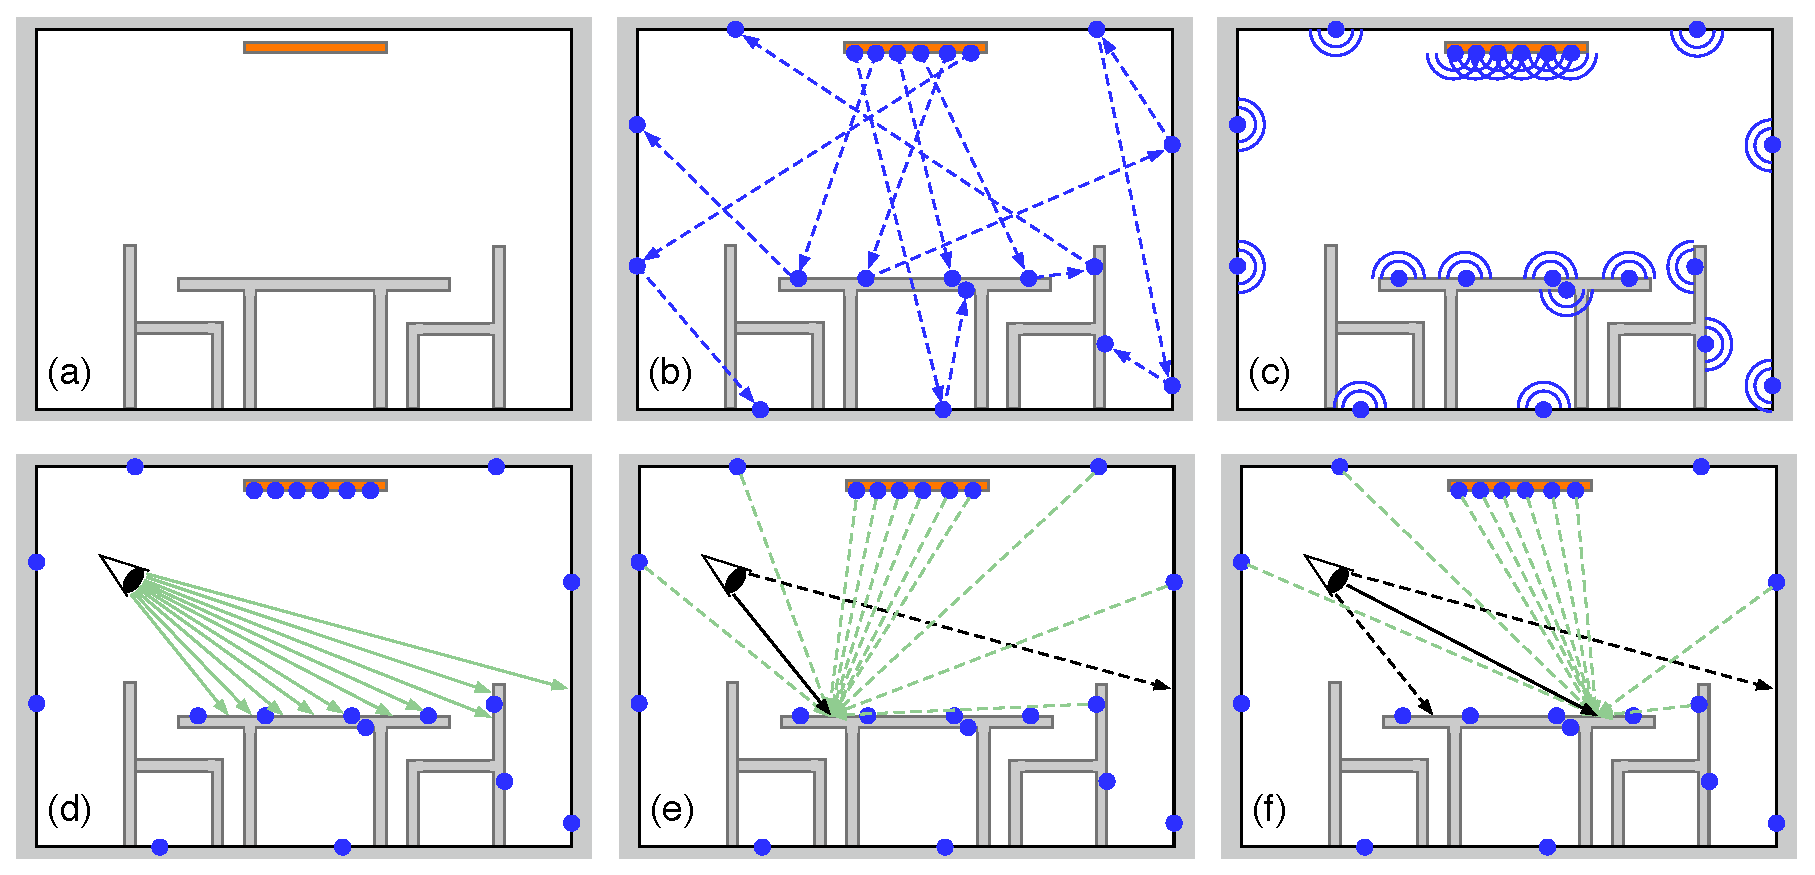
\includegraphics[width=1.0\thewidth ]{figures/ir/instant-radiosity}
	\caption{即时辐射度方法:为了能够即时的计算场景(a)中的辐射度(即间接漫反射光照),一些少量的粒子从光源产生并在场景中传播(b),在每个粒子与场景的碰撞处产生一个虚拟点光源(c),在后续的渲染阶段,光线从摄像机发出并(可能经过一定镜面或光泽反射后)停留在漫反射表面上(d),在每个观察点处,其辐射照度可以直接通过对所有虚拟点光源的辐射亮度求和进行计算(e)和(f),当然和直接光照一样,每个点光源还需要计算阴影遮挡关系}
	\label{f:ir-instant-radiosity}
\end{fullwidth}
\end{figure}




\subsection{粒子的生成}


从表面上看,即时辐射度中的虚拟点光源很像光子映射中的光子,例如都是从光源出发并最终落于漫反射表面而形成。然而实际上它们存在一些重要的差别。

首先,光子映射中的光子是可以经过光泽或镜面表面的,这方面和双向路径追踪是完全一致的,而唯一不同的是两条子路径的连接与合并的处理,合并的操作使光子映射拥有了处理焦散效果的能力;而即时辐射度中的粒子仅与漫反射表面交互\footnote{尽管后面介绍的即时辐射度方法也可以扩展至光泽表面,但是这里我们首先聚焦于理解即时辐射度方法的基本思路,所以暂时假设粒子只经过漫反射表面。},所以虚拟点光源携带的只有间接漫反射光照,因此这也意味着即时辐射度不具备处理焦散效果的能力。

其次,光子映射中的光子携带者相同(或相似)的能量,这是为了减少概率密度估计的误差,光子在传播过程中通过俄罗斯轮盘方法来保留光子的能量;而即时辐射度中的粒子携带的一般是辐射度,它们需要准确反映粒子的多次反弹结果,所以保留着粒子的真实“能量”。这也是这里称为“粒子”而不是“光子”的原因。

最后,也是最重要的一点,光子密度对光子进行密度估计以计算辐射亮度,而即时辐射度将粒子视为一个普通的光源,因此即时辐射度中两条子路径的的连接与传统的双向路径追踪是一致的,只不过双向路径追踪中每个摄像机子路径仅与少量光源子路径连接,而即时辐射度中每条摄像机子路径与所有光源子路径连接。

正是由于粒子仅携带间接漫反射光照,而且环境的间接漫反射光照分布往往非常平滑,所以才可以使用非常少量的虚拟点光源来近似间接漫反射光照,这是即时辐射度方法相较于辐射度方法高效的原因,即时辐射度方法中的粒子数量通常要远小于光子映射中光子的数量。




\subsubsection{粒子的拟随机行走}
由于粒子的样本数量非常少,因此最好需要产生比较均匀的分布以减小样本的方差同时提高收敛的速度,\cite{a:InstantRadiosity}使用了霍尔顿序列来产生粒子的路径。霍尔顿序列是一种拟随机数,所以粒子的传播过程又称为拟随机行走(quasi-random walk)\myindex{拟随机行走}{quasi-random walk}\cite{a:Quasi-MonteCarloRadiosity}。

霍尔顿序列可以高效地生成指定维数和数量的随机数序列,相关知识请参见第\ref{sec:quasi-monte-carlo}节的内容,为了思维的连贯性,这里对其做一个简单回顾。对于$N$个$s$维的随机数$x_0,\cdots,x_{N-1}\in [0,1)^{s}$,其霍尔顿序列为:

\begin{equation}\label{e:ir-halton-sequence}
	x_i=(\Phi_{b_1}(i),\cdots,\Phi_{b_s}(i))
\end{equation}

\noindent 这里$b_j$表示第$j$个素数,由于$x_i$是$s$维的,所以$\Phi_{b_j}(i)$表示第$i$个随机数中的第$j$维分量。通过上式,给定一个整数$i$和维度$s$,便可以获得其对应的霍尔顿序列表示的随机数。

这些随机数被用于路径追踪中的方向,位置采样等用途。然而霍尔顿系列并不可以动态调整维度,即是说我们需要首先确定维度然后才能产生随机数,这和路径追踪的过程是不符的:一个粒子在传播过程中实现并不知道什么时候会被吸收,因此无法确定路径的维度。因此为了使用霍尔顿序列随机数,我们需要一种机制找出每条路径的长度。

递归的渲染方程可以写为诺依曼级数(Neumann series)\myindex{诺依曼级数}{Neumann series}的形式,即:

\begin{equation}\label{e:ir-transport-operator}
	L=(I-T_{f_r})^{-1}L_e=\sum^{\infty}_{j=0}T^{j}_{f_r}L_e
\end{equation}

\noindent 这里$j$表示路径的长度。本质上,上述的诺依曼级数将光照贡献按照路径长度分为不同的部分,因为所有具有相同固定长度的路径具有相同的积分形式,因此其光照传输的过程可以使用一个相同的传输操作符$T^{j}_{f_r}$代替。从这里也可以看出,传输操作符(transport operator)\myindex{传输操作符}{transport operator}的意义其实就是对来自光源$L_e$中的光子执行$j$次反射之后,还剩多少能量被保留下来。

将式\ref{e:ir-transport-operator}代入式\ref{e:ir-average-radiance}中,在辐射度设置下可以得到传输操作符的函数为:

\begin{equation}
\begin{aligned}
	T_{mn}L=& \cfrac{1}{|P_{mm}|}\sum^{\infty}_{j=0}{\rm \int}_{P_{mn}}{\rm \int}_{\Omega^{j}}{\rm \int}_{S_e}p_j(y_0,\vec{\omega}_0,\cdots,\vec{\omega}_j)\\
	&V(y_j,y^{'})f_{\rm d}(y^{'}) \cfrac{\cos\theta_j\cos\theta^{'}}{|y_j-y^{'}|^{2}}{\rm d}y_0{\rm d}\omega_0\cdots {\rm d}\omega_jdP
\end{aligned}
\end{equation}

\noindent 这里$S_e$表示光源上所有光照值不为0的区域,$y^{'}=h(y_f,P-y_f)\in S$表示摄像机位置($y_f$)通过屏幕上的位置$P\in P_{mn}$击中场景的第一个点的位置,$V(y_j,y^{'})f_d(y^{'})$表示点$y_i$和点$y^{'}$之间的可见性。上式中的辐射亮度密度$p_j$为:

\begin{equation}\label{e:ir-radiance-density}
	p_j(y_0,\vec{\omega}_0,\cdots,\vec{\omega}_j):=L_e(y_0)\prod^{j}_{l=1}(\cos\theta_{l-1}f_d(y_l))
\end{equation}

\noindent $p_j$表述的是经过$j$次反射之后的辐射亮度。这里$y_0\in S_e$是位于光源上的点,后续的点$y_{l+1}$可以由$y_l$通过光线投射决定,即$y_{l+1}=h(y_l,\vec{\omega}_l)$,其中$0\leq l<j$。

由于余弦函数的乘积形式的分布是非常平坦的,所以式\ref{e:ir-radiance-density}表面,在辐射度设置下,传输操作符可以使用场景中漫反射系数的平均值近似,即:

\begin{equation}\label{e:ir-mean-reflectivity}
	\overline{\rho}:= \cfrac{\sum^{k}_{k=1}\rho_{d,k}|A_k|}{\sum^{k}_{k=1}|A_k|}\approx ||T_{f_d}||
\end{equation}

\noindent 这里$S=\bigcup^{K}_{k=1}A_k$表示所有场景中的表面,$\rho_{d.k}$表示第$k$个表面$A_k$的平均漫反射系数。

有了式\ref{e:ir-mean-reflectivity}对漫反射传输操作符$T_{f_d}$的近似表述,我们可以使用部分吸收(fractional absorption)\myindex{部分吸收}{fractional absorption}而不是俄罗斯轮盘吸收(Russian Roulette absorption)\myindex{俄罗斯轮盘吸收}{Russian Roulette absorption}(参见第\ref{sec:russian-roulette}节的内容)的方式来决定粒子的传输次数(即路径的长度)。即对于$N$个从光源发出的粒子,有$\overline{\rho}N$个粒子在第一次反射的时候不会被吸收,有$\overline{\rho}^{2}N$个粒子会在第二次反射的时候存活下来,以此类推,从光源发出的$N$的粒子一共可以产生的粒子数量$M$是有限的,即:

\begin{equation}
	M<\sum^{\infty}_{j=0}\overline{\rho}^{j}N= \cfrac{1}{1-\overline{\rho}}N=:\overline{l}N
\end{equation}

\noindent 上式表面总共的粒子数量是与$N$成线性关系的,这里$\overline{l}$表示平均路径长度。

有了这种路径的长度区分,我们就知道了路径的长度,因此霍尔顿序列可以被很容易地运用于路径追踪中,只需要把相同长度的路径提取出来使用同一个对应维度的霍尔顿序列作为随机数即可。例如,由于只有$\overline{\rho}N$个粒子被反射,因此$N$个粒子中只有$(1-\overline{\rho})N$个粒子使用1维霍尔顿序列,其传输操作符为$T_{mn}$(即摄像机直接可见的表面点处的漫反射系数),而$\overline{\rho}N$个粒子使用2维霍尔顿序列,其传输操作符为$T_{mn}T_{f_d}$,以此类推。




\subsection{算法实现}\label{sec:ir-implementation}
以上我们介绍了即时辐射度方法的一些基本概念,现在便可以总结出基本的算法过程,如算法\ref{a:ir-instant-radiosity}所述,为了以低偏差顶点产生$p_j$的离散近似,算法\ref{a:ir-instant-radiosity}首先固定从光源上产生$N$个粒子,这些粒子分别使用第1和第2个素数(其素数分别为2和3)为底数产生的随机数作为光源上的位置采样,即$y=y_0(\Phi_2,\Phi_3)$,这些粒子的颜色值为$L=L_e(y)\text{ supp }L_2$\footnote{supp表示函数的支集,即所有非零值函数值的集合。}。

\begin{algorithm}
\begin{lstlisting}[language=C++,mathescape]
void InstantRadiosity(int $N$, double $\overline{\rho}$){
	double $\omega$, Start;
	int End, Reflections = 0; 
	Color $L$; 
	Point $y$; 
	Vector $\vec{\omega}$;
	
	Start = End = $N$; 
	while(End > $0$) {
		Start *= $\overline{\rho}$;
		for(int $i$ = (int) Start; $i$ < End; $i$++) {
			//选择光源上的起点位置
			$y=y_0(\Phi_2(i),\Phi_3(i))$;
			$L=L_e(y)*$ supp $L_e$;
			$\omega=N$;
		
			//粒子的多次反射
			for(int $j$ = 0; $j$ <= Reflections; $j$++) {
				glRenderShadowedScene($ \cfrac{N}{\lfloor\omega\rfloor}L,y$); 
				glAccum(GL_ACCUM, $ \cfrac{1}{N}$);
				//产生漫反射方向
				$\vec{\omega}=\vec{\omega}_d(\Phi_{b_{2j+2}}(i),\Phi_{b_{2j+3}}(i))$;
				//按采样的漫反射方向得到新的顶点
				$y=h(y,\vec{\omega})$;
				//按漫反射系数对辐射亮度进行消减
				$L*=f_d(y)$;
				$\omega *=\vec{\rho}$;
			}
		}
    
		Reflections++;
		End = (int) Start;
	}
	
	glAccum(GL RETURN, 1.0);
}                                                                                
\end{lstlisting}	
\caption{即时辐射度算法的伪代码}
\label{a:ir-instant-radiosity}
\end{algorithm}

在算法\ref{a:ir-instant-radiosity}中,不同路径长度的粒子被组合在一起,后续的路径追踪涉及对反射方向的采样,相应维度的随机数均可以从式\ref{e:ir-halton-sequence}计算而出。注意霍尔顿序列随机数表示的是一个单位超立方体$[0,1]^{s}$上的一个点,所以相邻两个随机数分量可以按如下式被转化为服从cosine分布的方向:

\begin{equation}
	\vec{\omega}=\vec{\omega}_d(\Phi_{b_{2j+2}},\Phi_{b_{2j+3}})=(\arcsin\sqrt{\Phi_{b_{2j+2}}},2\pi \Phi_{b_{2j+3}})
\end{equation}

\noindent 在每一个光线投射的交点$y=h(y,\vec{\omega})$,粒子的辐射亮度被对应表面的漫反射系数$f_d(y)$消减。算法\ref{a:ir-instant-radiosity}按路径的长度分组进行处理,首先从第$\overline{\rho}N$到$N$个长度为0(即位于光源上)的粒子被产生,接着从第$\overline{\rho}^{2}N$到$\overline{\rho}N$个长度为1的粒子被处理,以此类推,直到所有$N$条路径被处理完毕。

所有粒子被按照直接光照的方式进行渲染,这通过调用glRenderShadowedScene使用图形硬件进行处理。但随之而来的问题是,我们希望所有的粒子的光照都同等的重要,而直接使用辐射亮度的绝对值进行渲染会使得多次反弹的粒子的光照贡献非常小。所以这里使用了类似复合重要性采样的方式对所有粒子的光照结果进行加权,即每个粒子的光照被乘以了一个权重系数$ \cfrac{N}{\lfloor\omega\rfloor}L$。

每个粒子的光照都被使用GL\_ACCUM累加起来,由于每个像素都被每个粒子照射,所以最终的像素累积颜色值被乘以$ \cfrac{1}{N}$以求其平均值。

图\ref{f:ir-instant-radiosity-example}展示了辐射度算法的过程,左边两列分别展示了$N=10$个光源上的粒子(红色圆点)及其光照结果,中间两列展示了一次反射的粒子及其光照结果,右边A,B和C分别表示不同的$N$值对应即时辐射度光照的累积结果。

\begin{figure}
\begin{fullwidth}
	\begin{subfigure}[b]{0.38\thewidth}
		\includegraphics[width=1.0\textwidth]{figures/ir/ir-1-1}
		\caption{$\langle L_e,\Psi_{mn} \rangle+T_{mn}L_e$}
	\end{subfigure}
	\begin{subfigure}[b]{0.37\thewidth}
		\includegraphics[width=1.0\textwidth]{figures/ir/ir-1-2}
		\caption{$+T_{mn}T^{n}_{f_d}L$}
	\end{subfigure}
	\begin{subfigure}[b]{0.235\thewidth}
		\includegraphics[width=1.0\textwidth]{figures/ir/ir-1-3}
		\caption{results}
	\end{subfigure}
\end{fullwidth}
\caption{即时辐射度方法中粒子的拟随机行走过程,其中(a)和(b)分别展示了0次和1次反射粒子的光照结果,(c)展示了不同$N$值对应的粒子累积结果,这里$\overline{\rho}=0.5774$,结果图像中的$N$值分别取$N\in\{ 10,32,64\}$(图片来自\cite{a:InstantRadiosity})}
\label{f:ir-instant-radiosity-example}
\end{figure}




\subsubsection{总~~结}
除了上述的基本算法,\cite{a:InstantRadiosity}还提到了对几个小的扩展。首先霍尔顿系列产生的随机数是与网格对齐的(即位于网格的边上),这样的样本分布任意导致走样,为了每个倒根函数$\Phi_b$被使用了一个随机的抖动$\Phi_b+ \cfrac{\xi}{N}$,这里$\xi$为一个随机数;此外,为了增加对光泽/镜面反射效果的处理,可以通过修改$T_{mn}$为一般的BRDF函数$f_r$来实现,但是这要求更高数量的粒子,因为光泽/镜面反射的分布要尖锐得多,我们将在后面进一步讨论对全频率BRDF函数的处理。

通过本节的内容可以看出,即时辐射度是一种简单而高效的方法。例如它只需要将间接漫反射光照表述为光源子路径中的一些顶点即可,并且这些粒子的光照被即时处理,并不需要占用大量的内存,唯一需要的是一个较大的图像空间的缓冲区;同时通过将间接漫反射光照转换为直接光源,其光线是连贯的,光照的计算可以使用图形硬件的光栅化能力。

然而即时辐射度方法也有一些缺点,例如它主要集中于漫反射交互,因此很难处理和光泽/镜面反射相关的一些现象(如焦散效果);其次,虽然对光照的离散化没有直接暴露在摄像机面前,但是每个粒子都当做一个点光源,这些点光源将产生硬阴影,较少的粒子数量会使这种硬阴影的分布非常明显,因此多少粒子数量是合适的也是需要小心考虑的问题;最后,由于式\ref{e:ir-transport-operator}中的分母向包含了两个点$y_j$和$y^{'}$之间的距离,这将距离非常近(例如墙角)的区域产生奇异值。

以上这些都是本章后面需要讨论和克服的问题。





\section{近似方法}\label{sec:ir-improved-algorithms}
本质上,即时辐射度方法是一种双向路径追踪算法,但是它主要聚焦于(间接)漫反射光照,并且使用拟蒙特卡洛积分来加速光照计算以及积分的收敛速度,这使得它仅仅只需要少量的路径样本(例如几百个)就可以达到很好的效果,它是能够产生高质量图像的四大\footnote{其他三个为路径追踪,光子映射以及后面会介绍的辐射照度缓存技术。}全局光照技术之一。

基于即时辐射度方法的基本思路,一些扩展或增强方法被提出,这些方法聚焦于不同的层面和目的,例如其中一些方法使用更粗略的近似以达到交互式渲染的需求,一些方法尝试使用即时辐射度方法处理全频率的光照效果,一些聚焦于自适应地调整粒子的密度分布,以及提高粒子的数量以增强图像的质量。本节我们首先讨论第一类扩展方法,其他扩展方法则会在后续的内容中被讨论。




\subsection{反射阴影图}\label{sec:ir-RSM}
在原始的即时辐射度算法中,光源子路径阶段中的每个粒子都是按照路径追踪中的一条光线一条被发射,所以每个粒子需要执行代价比较高的光线和场景的相交计算。然而对于一些情况,例如交互式预览的需求,通常并不需要那么高的精度,此时,一些更粗略的近似即可满足需求,例如只包含一次反弹的间接漫反射光照。

基于上述观察,\cite{a:ReflectiveShadowMaps}提出了反射阴影图(reflective shadow map,RSM)\myindex{反射阴影图}{reflective shadow map}, 它使用一个阴影图来表述虚拟点光源。其中在第一个介绍,它将摄像机置于光源上的某个点对场景进行渲染以产生一个阴影图,但是除了存储传统表面的深度值,它还对其进行扩展以存储这些点反射的光照值,因此称为反射阴影图。在反射阴影图中,每个像素被当做一很小的面积光源,这相当于前面介绍的虚拟点光源;在后续的渲染阶段,每个可视点收集所有这些反射阴影图中的像素的光照以产生一次反弹的间接光照。




\subsubsection{数据生成}
RSM的生成和传统的阴影图很类似,但是它需要使用多重渲染目标(multiple-render targets),因为除了需要深度缓冲存储深度值$d_p$之外,它还需要额外的缓冲对象存储法线$n_p$,世界坐标$x_p$,以及辐射通量$\Phi_p$。RSM中的每个像素称为一个像素光源(pixel light)\myindex{像素光源}{pixel light},它们表示场景中的一次反弹间接光照。

\begin{figure}
\sidecaption
	\includegraphics[width=.65\textwidth]{figures/ir/ir-2-1}	
	\caption{两个反射阴影贴图中的像素$p$和$q$分别对应两个间接像素光源$x_p$和$x_q$}
	\label{f:ir-rsm}
\end{figure}

在图\ref{f:ir-rsm}中,如果假设像素光源的面积无限小,则其反射至方向$\omega$的辐射强度(单位$W/sr$)可以使用余弦辐射定理表述,即:

\begin{equation}\label{e:ir-diffuse-radiant-intensity}
	I_p(\omega)=\Phi_p \max\{ 0,\langle n_p,\omega \rangle \}
\end{equation}

\noindent 因此位于$x$处法线为$n$的单位面积由于像素光源$p$接受到的辐射照度(单位$W/m^{2}$)为:

\begin{equation}
\begin{aligned}
	E_p(x,n)&= \cfrac{I_p(\omega)}{r^{r}} \\
			&=\Phi_p \cfrac{\max\{0,\langle n_p,x-x_p \rangle\}\max\{0,\langle n,x_p-x \rangle \}}{||x-x_p||^{4}}
\end{aligned}
\end{equation}

因此,与前面存储辐射亮度的虚拟点光源不同,像素光源直接存储的是辐射通量$\Phi_p$。通过这样的表述,像素光源不必关心其该像素对应光源的面积表述,这使像素光源的生成和计算更简单。




\subsubsection{计~~算}\label{sec:ir-rsm-sampling}
表面上位于$x$处法线为$n$的点的间接辐射照度可以通过对所有像素光源光照的加和而实现(注意这里暂时没有考虑间接光照的阴影遮挡,我们会在后面的内容中介绍阴影遮挡的处理),即:

\begin{equation}
	E(x,n)=\sum_{p}E_p(x,n)
\end{equation}

\noindent 阴影图的分辨率通常比较高,而表面上的每个点都要向所有像素光源收集光照,为了达到交互式需求,我们需要将对像素光源的加和限制到一个的数量范围内,例如$300~400$,多个像素光源即可以达到很好的近似效果。\cite{a:ReflectiveShadowMaps}使用了一种重要性驱动的方法,从而将对粒子的采样集中在相关的像素光源上。

\begin{figure}
\sidecaption
	\includegraphics[width=.65\textwidth]{figures/ir/ir-2-2}	
	\caption{反射阴影贴图的采样}
	\label{f:ir-rsm-sampling}
\end{figure}

其采样的思路如图\ref{f:ir-rsm-sampling}所示,$x$点并没有直接被照射,所以它在阴影图中是不可见的,如果我们将点$x$投影到阴影图中,则在世界空间内相邻近的像素光源在阴影图上仍然会保持这种相邻性,这里$x_{-1}$和$x_{-2}$都是相对比较靠近$x$的,然而它们的法线方向和$x$的法线方向相反,所以它们对$x$并没有光照贡献,同样虽然$x_1$也比较靠近$x$,但是它们位于同一平面上,所以也不会产生间接光照贡献,所以最相关的像素光源就是$x_2$。

一般情况下,阴影图上$x$与一个像素光源$x_p$的距离可以很好地用来近似它们在世界空间中的距离。如果它们之间的深度值具有较大的差异,则它们在世界空间中的距离可能非常大,这使得对应像素光源的光照影响被高估,然而,由于具有相似重要性的像素光源在阴影图上总是相近的,所以阴影图上距离的重要性仍然是一种有效的采样依据。

为了实现对像素光源按阴影图上的距离进行重要性采样,首先$x$被投影到阴影图中,其位置为$(s,t)$,然后位于$(s,t)$附近的像素光源被选取,其采样的概率密度与像素光源到$(s,t)$之间的距离的平方成反比。这种采样很容易在极坐标中实现,以$(s,t)$为中心,可以使用以下位置密度对像素光源进行采样,即:

\begin{equation}
	(s+r_{\max}\xi_1 \sin(2\pi \xi_2),t+r_{\max}\xi_1\cos(2\pi\xi_2))
\end{equation}

\noindent 这里$\xi_1$和$\xi_2$为均匀分布的随机数,其采样的模式可以参见图\ref{f:ir-rsm-sampling-pattern}所示。由于仅与阴影图中的纹理坐标位置相关,这样的采样模式可以被预计算并被存储起来供所有间接光照计算的使用。

\begin{figure}
\sidecaption
	\includegraphics[width=.35\textwidth]{figures/ir/ir-2-3}
	\caption{一个采样模式的示例,在这个示例中,随着离中心的距离增大,其采样密度会减少,而样本的权重则会增加,这里其权重被视觉化为原点半径的大小}
	\label{f:ir-rsm-sampling-pattern}
\end{figure} 




\subsubsection{屏幕空间插值}
尽管上面介绍的基于阴影图中纹理位置距离的重要性采样方法使得单个像素需要计算的像素光源的数量大大减少,由于最终图像空间的每个像素都要进行光照计算,这样的计算成本仍然非常高,为了进一步提升效率,\cite{a:ReflectiveShadowMaps}使用了一种基于屏幕空间的插值方法。

该方法将渲染阶段分离成了三个阶段,首先,一个低分辨率的图像被渲染,这些图像空间中的每个像素使用正常的流程对其计算间接漫反射光照;然后,一个全分辨率的图像被渲染,但是此时它并不使用像素光源来计算间接光照,而是尝试使用前面低分辨率的图像结果对其进行插值计算,其插值的依据是检查该像素与低分辨率图像中相邻的像素是否具有相似的法线方向,以及它们在世界空间内的位置是否相近,如果满足这一的条件,则该像素的值直接通过低分辨率的图像进行插值计算,否则不对该像素进行任何处理;最后,所有未被插值处理的像素被使用像素光源进行间接漫反射光照的计算。

\begin{figure}
\sidecaption
	\includegraphics[width=.45\textwidth]{figures/ir/ir-2-4}
	\caption{屏幕空间插值计算的效率分布,在那些红色的像素区域,应该尽可能少使用插值}
	\label{f:ir-rsm-ss-interpolation}
\end{figure} 


Figure \ref{f:ir-rsm-ss-interpolation}显式了这种插值方法的效率,仅仅那些红色的像素需要从像素光源计算间接光照,因为这些区域的法线变化比较大,其间接漫反射光照的变化也可能比较大,大部分的平坦的区域则可以使用低分辨率的图像进行光照计算,然后通过插值计算每个像素的间接光照。





\subsection{溅射法}\label{sec:ir-splatting}
基于反射阴影图,\cite{a:SplattingIndirectIllumination}介绍了溅射间接光照(Splatting Indirect Illumination)\myindex{溅射间接光照}{Splatting Indirect Illumination}法,与反射阴影图法相比,它有三点改进:

\begin{itemize}
	\item 首先,与RSM从每个可见点收集(gathering)来自像素光源的光照不同,溅射法在一个延迟着色阶段使用发射(shooting)的方法来计算间接光照,即对于每一个像素光源,它将其光照贡献溅射到其屏幕空间的相邻像素。这种方法也能够更好地限制每个像素光源影响的范围区域。
	\item 其次,一个更高效的基于GPU的重要性采样方法被运用于像素光源的选择。
	\item 更进一步,它允许对光泽表面计算间接光照,这使得可以同时计算间接漫反射光照和焦散效果。
\end{itemize}




\subsubsection{非漫反射表面}
为了渲染来自光泽表面的间接光照和焦散效果,像素光源的光照发射必须满足非漫反射的特征,图\ref{f:ir-glossy-pixel-light}显式了位于漫反射和光泽表面的像素光源的光照发射方式。

\begin{figure}
	\sidecaption
	\includegraphics[width=0.65\textwidth]{figures/ir/ir-3-2}
	\caption{漫反射(左)和光泽表面(右)上像素光源发射的能量}
	\label{f:ir-glossy-pixel-light}
\end{figure}

对于Phong模型的表面,光泽的像素光源发射的辐射强度可以表述为:

\begin{equation}\label{e:ir-phong-radiant-intensity}
	I_p(\omega)=\Phi_p \max\{ 0,\langle r_p,\omega\rangle \}^{P}
\end{equation}

\noindent 这里$r_p$表示像素光源$p$的主要反射方向,每个光泽像素光源的$r_p$值可以被预存起来,$P$表示Phong指数。

\begin{figure}
\sidecaption
	\begin{subfigure}[b]{.315\textwidth}
		\includegraphics[width=1.0\textwidth]{figures/ir/ir-3-4}
	\end{subfigure}
	\begin{subfigure}[b]{.315\textwidth}
		\includegraphics[width=1.0\textwidth]{figures/ir/ir-3-5}
	\end{subfigure}
\caption{焦散的实时渲染}
\label{f:ir-non-diffuse-surfaces}
\end{figure}

由于光泽反射的方向分布形状更加狭窄,所以一个正方形的区域显然是比较浪费的,所以每个像素光源被使用一个更紧凑的包围几何形状(这将在下一节讨论),有了这样紧凑的包围区域,间接光泽反射光照可以以类似间接漫反射光照的速度被计算。通常,光泽反射要求更高数量的像素光源,但是其影响的像素区域也更小,这可以带来一定的补偿。图\ref{f:ir-non-diffuse-surfaces}显式了非漫反射表面光照以及焦散效果的一个示例。



\subsubsection{重要性采样}
由于光泽反射通常导致光照分布的频率变化比较大,因此往往需要更多的样本才能更好地近各种全局光照效果,所以在具有非漫反射表面的场景中,重要性采样尤其重要。为了使对RSM的采样模式更好地适配像素光源的辐射通量分布,这里使用的是由\cite{a:WaveletImportanceSampling}提出的阶层式变形(hierarchical warping)\myindex{阶层式变形}{hierarchical warping}方法。 

在阶层式变形方法中,首先所有样本位置被均匀分布于整个阴影图空间,然后开始对阴影图进行阶层划分,每一级将阴影图划分为四个大小相同的区间,并计算每个区间相对于整个阴影图的辐射通量比例,如图\ref{f:ir-hierarchical-warping}(a)所示,其每个四分之一区间所占的辐射通量比例分别为$30\%,50\%,15\%和5\%$。

\begin{figure}
\begin{fullwidth}
	\includegraphics[width=1.0\thewidth]{figures/ir/ir-3-1}
	\caption{阶层式变形方法中一个层级内按重要性变形的过程}
	\label{f:ir-hierarchical-warping}
\end{fullwidth}
\end{figure}

然后,每一个阶层的变形由垂直和水平变形组成,其变形的依据是其辐射通量的分布,例如对于垂直变形,由于图\ref{f:ir-hierarchical-warping}上下两部分的辐射通量比例分别为$80\%=30\%+50\%$和$20\%=15\%+5\%$,所以它首先将阴影图在垂直方向上按面积分成80\%和20\%两个区域,如图\ref{f:ir-hierarchical-warping}(b)所示,然后将这条分割线挤压至垂直方向的中点,使阴影图被分割为相等的两半,如图\ref{f:ir-hierarchical-warping}(c)所示,这样就使得垂直方向上的样本分布服从其辐射通量的分布。根据类似的过程,在对水平方向执行样本的挤压使其服从水平方向的辐射通量分布,如图\ref{f:ir-hierarchical-warping}(d)所示,最后的样本密度分布如图\ref{f:ir-hierarchical-warping}(e)所示,它和图\ref{f:ir-hierarchical-warping}(a)所示的辐射通量分布是一致的。

由于该方法是通过移动样本的位置来得到最终的样本位置分布,所以样本的最终位置不能通过对某个密度函数进行采样得到,它们也必须经历一个变换过程。首先通过对阴影图均匀采样得到的样本位置为$s_i=(x_i,y_i)$,其中$x_i,y_i\in[0,1)$,其对应的样本权重为$w_i=1$。当这些样本被挤压至新的位置之后,根据挤压的过程,样本新的位置$y^{'}_i$可以由下式得出(以垂直挤压为例):

\begin{equation}
	y^{'}_i=\begin{cases}
		y_i/(2\Phi_r) &\text{if }y_i<\Phi_r\\
		(1+y_i-2\Phi_r)/(2(1-\Phi_r)) & \text{ 其他}
	\end{cases}
\end{equation}

\noindent 这里$\Phi_r= \cfrac{\Phi_{top}}{\Phi_{top}+\Phi_{bottom}}$,它表示垂直方向上按辐射通量比例得到的阴影图上的位置,如图\ref{f:ir-hierarchical-warping}(b)中上下两部分的水平分界线。为了补偿采样密度的变化,每个样本对应的权重系数也需要发生改变以使所有的样本总的权重保持不变:

\begin{equation}
	w^{'}_i=\begin{cases}
		w_i/(2\Phi_r)     & \text{if }y_i<\Phi_r \\
		w_i/(2(1-\Phi_r)) & \text{ 其他}
	\end{cases}
\end{equation}

\noindent 上述的变换得到了经过变换后的样本分布,使用类似的思路可以对样本进行水平方向的位置变换,这得到了一个新的阶层划分,通过重复迭代上述的过程,可以得到一个阶层式的密度分布,使得最高分辨率的密度分布能够更好地近似像素光源的辐射通量分布。经过变形后的采样模式(如图\ref{f:ir-hierarchical-warping}(e)所示)被用于对RSM中像素光源的采样,每个像素光源在对表面产生光照之前需要被乘以每个样本的权重值$w^{'}_i$。




\subsubsection{紧凑的包围盒几何体}
在溅射法中,每个像素光源被执行一个全屏的像素着色器,然而一个像素光源通常仅对它周围的表面产生较为显著的光照贡献,因此我们有必要针对每个像素的BRDF分布产生一个更紧凑的包围盒几何体,然后仅仅对该几何体执行一次像素着色器,这将大大提高渲染性能。而这个包围盒几何体的计算可以使用一个成本较低的顶点着色器来实现。

我们的目标是产生一个简单的包围盒区域,使得处于该包围盒外部的光照值小于某个较小的阈值。如图\ref{f:ir-bounding-geometry}所示,对于一个漫反射像素光源,这个包围区域为一个蛋形的形状,而对于光泽表面,其形状近似为一个Phong叶片。

\begin{figure}
	\sidecaption
		\includegraphics[width=0.65\textwidth]{figures/ir/ir-3-3}
	\caption{使用简单的包围盒要近似漫反射(左)和光泽反射(右)表面像素光源的分布}
	\label{f:ir-bounding-geometry}
\end{figure}


出于效率考虑,通常我们并不会计算出精确的包围盒区域,在\cite{a:SplattingIndirectIllumination}中使用椭球体来近似每个像素光源的影响区域,该椭球体同时处理漫反射和非漫反射像素光源,然后渲染的时候可以使用一个球形的三角网格来代替全屏四边形渲染。

我们可以使用中心位于$p$的球面坐标来表示像素光源$p$的光照影响区域,其中该包围区域所形成几何体的每个点由一个方向$\omega$和一个距离$r$描述,如图\ref{f:ir-pixel-light-region}左边小图所示。对于场景中的任意一点$(\omega,r)$,其接收来自像素光源$p$的辐射照度由三个参数决定:$\omega$,该点与像素光源的距离$r$,以及入射光方向与该点法线夹角的余弦$\cos\beta$,但是由于我们无法提前知道$\beta$的值,所以只能将其限制在取值范围内,我们可以将点$(\omega,r)$处的辐射照度限制在$I_p(\omega)/r^{2}$以内,如图\ref{f:ir-pixel-light-region}所示。

\begin{figure}
	\sidecaption
	\includegraphics[width=0.65\textwidth]{figures/ir/ir-3-6}
	\caption{左:一个像素光源涉及的光照计算,右:不同指数对应的反射方向分布}
	\label{f:ir-pixel-light-region}
\end{figure}

通过这种方式,漫反射和光泽反射光源都可以统一到一起,其中$\alpha$对于漫反射表面表示光线与法线$n_p$的夹角(如式\ref{e:ir-diffuse-radiant-intensity}),而对于光泽表面表示光线与(像素光源)反射方向$r_p$的夹角(如式 \ref{e:ir-phong-radiant-intensity}),这种关系如图\ref{f:ir-glossy-pixel-light}所示。如果我们对漫反射表面使用指数$n = 1$,则辐射照度可以被限制在极坐标方程$B(\alpha,r) = I_0 \cos(\alpha)^{n}/r^{2}$内。

像素光源$p$的影响范围可以被限定在方程表示的等位面$B(\alpha,r) = I_{low}$.,内,如图\ref{f:ir-pixel-light-region}分别显示了Phong指数为1,10和100时的等位面,其中$I_0 = 1, I_{low} = 1$。

上述的光源限制范围几何形状可以使用一个椭球体包围,该椭球体对应的参数可以由一个简单的启发式得出,参见\cite{a:SplattingIndirectIllumination}。图 \ref{f:ir-ellipses}中的灰色线段显示了这种椭球体,其黑色线段表示像素光源原始的包围范围。

\begin{figure}
	\begin{center}
		\includegraphics[width=\textwidth]{figures/ir/ir-3-7}
	\end{center}
	\caption{用椭球形状来简单地近似像素光源的分布}
	\label{f:ir-ellipses}
\end{figure}




\subsection{不完全阴影图}\label{sec:ir-ISM}
在传统的即时辐射度方法中,每个虚拟点粒子完全被当做一个“光源”,每个光源对整个场景中的表面点进行照射,我们可以通过传统的(高分辨率)阴影图或者光线投射来计算每个虚拟点光源与表面点之间的可见性,然而由于这些高精度可见性计算的成本非常高,所以往往不能达到交互式的需求。

为了对虚拟点光源提供一种高效的阴影计算机制,\cite{a:ImperfectShadowMapsforEfficientComputationofIndirectIllumination}提出了不完全阴影图(imperfect shadow map,ISM)\myindex{不完全阴影图}{imperfect shadow map},它基于这样的观察,即虽然高频的直接光照需要精度非常高的可见性信息,但是间接光照的频率变化却非常平滑,因此每个虚拟点粒子可以使用一个低分辨率的阴影图来近似其可见性信息,我们称这种低分辨率的阴影图为不完全阴影图,不完全阴影图可以使用现代图形处理器高效地计算。




\subsubsection{场景预处理}\label{sec:ir-point-based-representation}
为了后面高效地计算不完全阴影图,在一个预处理阶段,我们首先将整个3D场景近似为一个基于点的几何表述,这些点仅仅用于可见性(而不是着色)的计算,它们通过这样的方式产生:首先根据面积比例概率均匀地选择一个三角形,然后再从该抽样的三角形面积中随机选取一个位置。

为了便于后续的计算,每个点需要同时存储下其所在三角形的索引,该点在该三角形的质心坐标(barycentric coordinate)\myindex{质心坐标}{barycentric coordinate},这些信息可以用于获取该点的法线,反射系数等信息。




\subsubsection{ISM的创建}
在传统的阴影图中,摄像机首先被置于光源的位置,然后对整个场景执行一次光栅化渲染,深度缓冲区记录的深度值即为没有被遮挡的区域,超出该深度值的表面被遮挡。但是对于不完全阴影图,它渲染的是一个点(而不是几何网格)表述的场景,如图\ref{f:ir-imperfect-shadow-maps}中的红色和黄色圆点,此时上述的光栅化方法不再适用。为了创建一个不完全阴影图,点表述的场景被溅射到深度缓冲区上,每个点在深度缓冲区上溅射的面积由它到(虚拟点)光源距离的平方成反比。

\begin{figure}
	\includegraphics[width=\textwidth]{figures/ir/ir-4-2}
	\caption{使用不完全阴影图的全局光照效果:该场景中的间接光照被两个($\text{ISM}_0$和$\text{ISM}_1$)虚拟点光源表述,每个虚拟点光源使用基于点的场景表述生成一张阴影图,因为只需要粗略的可见性信息,所以每个虚拟点光源仅使用一部分(如图中红色和黄色点的区分)点来生成不完全阴影图,最后所有的虚拟点光源光照的加和表示最终的间接光照。右边上下两图展示了不完全阴影图的示例,其中较黑的区域表示较小的深度,较亮的区域表示较大的深度(图片来自\cite{a:ImperfectShadowMapsforEfficientComputationofIndirectIllumination})}
	\label{f:ir-imperfect-shadow-maps}
\end{figure}

当一个不完全阴影图被用于计算间接光照时,它需要覆盖整个半球面方向上的深度信息,即每个虚拟点光源向整个半球面方向上发射光照,因此不能使用传统阴影图使用的正交或投射投影,这里使用一种称为抛物线映射(parabolic mapping)\myindex{抛物线映射}{parabolic mapping}\cite{a:ShadowMappingforHemisphericalandOmnidirectionalLightSources}的方法来覆盖整个半球面上的深度信息。

另一点与传统阴影图不同的是,所有低分辨率的不完全阴影图被存储在一个单一的纹理中,如图\ref{f:ir-imperfect-shadow-maps}右边小图所示,并且它们全部在一个渲染通道中生成。为此,一个顶点着色器将输入的点集合数据流分别分配相同数量的点到每个不完全阴影图中,每个不完全阴影图只接受很少的一部分固定数量的点,这些点的选取是完全随机的,每个不完全阴影图的分辨率为$128\times 128$,它们全部被存储在一个分辨率为$4096\times 4096$的纹理中。

为了减少计算量,上述的过程只使用了很稀疏的点用于计算不完全阴影图,这使得深度图上可能留下没有被覆盖的“漏洞”。为此,一种推拉法(pull-push approach)\cite{a:PointSampleRendering,a:EfficientPointBasedRenderingUsingImageReconstruction}被运用于填补这些漏掉以重建为一个合理的深度图,它包括以下步骤:

\begin{itemize}
	\item 拉阶段(pull phase):拉阶段的主要目标是创建一个图像金字塔,这些图像通过对高分辨率的图像进行向下采样得到,每次相邻的4个像素被平均以得到一个低分辨率的图像,但由于高分辨率的图像存在漏洞,所以仅有那些“合法”(非漏洞)的像素值被用于平均计算。 
	\item 推阶段(push phase): 推阶段的主要目标是填充那些没有深度值的漏洞,这通过对低分辨率图像中相同位置处的像素进行插值计算来实现。
\end{itemize}

图\ref{f:ir-pull-push}展示了推拉法的效果,在实践中,只需要2,3级低分辨率图像即可达到比较满意的效果。

\begin{figure}
	\includegraphics[width=1.\textwidth]{figures/ir/ir-4-1}
	\caption{传统阴影图(左)与使用(右)和不使用(中)推拉法的不完全阴影图的对比,没有使用推拉法的不完全阴影图包含“漏洞”,这些漏洞在使用推拉法后可以达到比较好的结果(图片来自\cite{a:ImperfectShadowMapsforEfficientComputationofIndirectIllumination})}
	\label{f:ir-pull-push}
\end{figure}




\subsection{自适应不完全阴影图}\label{sec:ir-AISM}
不完全阴影图中虚拟点光源的分布和点集表述并没有考虑当前摄像机可见区域的分布,因此造成了一些计算资源的浪费,例如那些距离可见区域更近的虚拟点光源和视觉事件显然更加重要。以上分析可以总结为两个缺点:首先,由于虚拟点光源的选择没有考虑它们对最终图像的贡献,所以导致很多不必要粒子的计算;其次,类似的道理,均匀分布的场景点集表述也往往太过于稀疏,例如大量对当前视图可见性具有较小影响的区域占据了大量不必要的点数据。

为了应对这两个问题,\cite{a:MakingImperfectShadowMapsViewAdaptive}介绍了一种能够自适应视图的不完全阴影图方法,其视图自适应性是通过两种相互正交(不相关)的机制实现的,它们分别针对虚拟点光源和点集分布:首先,虚拟点光源的分布是与其对当前视图(current view)的光照贡献相关的,例如对当前视图越重要的虚拟点光源会得到更密集的采样;其次,针对间接光照可见性的场景点集表述(第\ref{sec:ir-point-based-representation}节)也是与当前视图相关的,对当前视图产生重要影响的几何细节会得到更精细的表述。

以下我们详细讨论视图自适应(view-adaptive)不完全阴影图的实现细节。




\subsubsection{双向反射阴影图}
在本节,我们首先讨论怎样生成视图自适应的虚拟点光源分布。

在路径追踪技术中,双向路径追踪相对于单向路径追踪能够自动寻找那些对摄像机非常重要的路径,具有某种“视图自适应”的能力,这种思路被运用于即时辐射度算法中以实现视图自适应,我们将在后面详细讨论这种双向即时辐射度技术\cite{a:BidirectionalInstantRadiosity}。然而,双向即时辐射度技术依赖于光线投射,其很难满足交互式的需求,\cite{a:MakingImperfectShadowMapsViewAdaptive}介绍了一种基于反射阴影图的技术,它既有反射阴影图的简单和高效,同时又具有双向即时辐射度算法的视图自适应能力。

首先,两个光栅化过程被分别执行。其中第一个光栅化过程将当前视图渲染至一个缓冲区,如图\ref{f:ir-adaptive-rsm}中的"View"和"Framebuf",其中Framebuf中的像素称为一个视图样本(view-sample);第二个光栅化过程则是以光源为视点生成一个反射阴影图,如图\ref{f:ir-adaptive-rsm}中的"Light"和"RSM"。这两个缓冲区中的每个像素都需要存储位置,法线和反射系数。

我们称反射阴影图中的像素为潜在虚拟点粒子(potential VPLs,pVPL),如图\ref{f:ir-adaptive-rsm}中的空心小圆圈所示,出于效率考虑,每个反射阴影图中可能只有部分pVPL会被选择成为真正的虚拟点光源,只有这些真正的虚拟点光源才会参与间接光照的计算,如图\ref{f:ir-adaptive-rsm}中的黄色圆点所示。 

为了实现视图自适应,这里不能再使用传统的基于出射辐射亮度的采样,而是基于当前视图定义了一个非均匀的概率分布,如图\ref{f:ir-adaptive-rsm}中的"Bi-dir. imp."所示,该概率分布能够估计虚拟点光源对视图样本的影响。

\begin{figure}
	\sidecaption
	\includegraphics[width=0.65\textwidth]{figures/ir/ir-5-1}
	\caption{双向反射阴影贴图组合了直接光照的重要性,以及其对帧缓存的贡献}
	\label{f:ir-adaptive-rsm}
\end{figure}

为了使该方法更加高效,这里引入两点简化:

\begin{itemize}
	\item 首先,这里依赖于一个随机的方案,每个pVPL仅仅对少量随机选择的视图样本执行光照影响计算($\approx 0.1\%$)。
	\item 其次,当计算每个pVPL光照影响的时候, 其忽略了可见性的影响。
\end{itemize}

基于上述的简化,每个pVPL便生成一个对一些随机选择视图样本(view samples)的平均贡献值,这些值被存储于另一个双向反射阴影图(bidirectional reflective shadow map,BRSM)\myindex{双向反射阴影图}{bidirectional reflective shadow map}当中,然后最终参与间接光照计算的VPL便从该BRSM中按其双向重要性进行选择。

这里为什么是双向的,是因为RSM中存储的样本其实表述的是光源子路径,而视图缓冲区中存储的样本则表示摄像机子路径,它们之间通过随机的视图样本选择而直接(忽略了可见性)相连而形成一条全路径,而每个pVPL样本的平均贡献值便对应于这些全路径相对于当前视图的重要性,这和双向路径追踪的思路类似,也因此BRSM中的pVPL分布即是服从当前视图情况的重要性分布,也即是图\ref{f:ir-adaptive-rsm}中的"Bi-dir. imp."缓冲区。

除了上述随机选择视图样本来计算pVPL的平均光照贡献,\cite{a:MakingImperfectShadowMapsViewAdaptive}还介绍了利用缓冲区中像素的空间分布特性来指导更好地选择pVPL的视图样本,这有点类似于反射阴影图技术中像素光源的采样,参见第\ref{sec:ir-rsm-sampling}节的内容,只不过这里是对视图缓冲区(而不是反射阴影图)进行采样,这里不再详述。

当然,为了方便对BRSM中的pVML进行采样,BRSM中存储的并不是直接的pVPL平均光照贡献值,而是存储每个pVPL与视图相关重要性分布的累积密度函数,这样便可以使用逆变换算法直接对BRSM进行采样。





\subsubsection{自适应不完全阴影图}
原始的不完全阴影图使用一个均匀分布的密度函数来对整个场景进行点采样,这使得不完全阴影图中漏掉的像素数量以及对漏掉填补的需求都大大增加,降低了处理大场景的能力。而实际上通过简单推理可知,较远遮挡物导致的间接光的阴影往往非常平滑,因此不必要使用太高精度对其进行表述;另一方面,少量较近的遮挡物在视图样本上却往往产生非常重要的阴影,它们的表述需要保持足够多的细节。

一个理想的遮挡物(稀疏点集)表述应该是考虑所有三角形和所有的视图样本之间的联系,但是这样的枚举过程显然很难满足交互式以及实时的需求,我们将在本章后面介绍这种更加精确的视图自适应方法,这里仅介绍一种高效的经验性的方法。

首先我们聚焦于一种简单的情形,即考虑场景中只包含一个视图样本$V$,因此我们的目标便是使对场景点采样的密度分布反比与这些点到$V$的距离,换句话说,越靠近$V$的三角形会得到更密集的采样。然而对场景点采样的过程包含首先对三角形采样,然后对三角形内部的点采样两个过程,而三角形是一个面积而不是一个点,所以我们无法估算一个面积到一个点的距离,所以这里使用从视图样本$V$观察到的每个三角形的立体角来估算该三角形面积对阴影的影响,因为立体角越大,其可能是一个靠近$V$较小的物体,也可能是一个离$V$较远但是面积较大的物体,这两种情况都对阴影的影响较大。所以通过三角形相对于视图样本$V$的立体角可以很好地用于估算该三角形于阴影的重要性,并且这种方法可以通过图形硬件很高效地实现。

首先,所有三角形被存储至一个三通道的三角形纹理(triangle texture)中,如图\ref{f:adaptive-ISMs}左边和中间小图所示,其每个纹素的三个通道分别用于存储一个顶点的三个(x,y,z)坐标值。基于上述三角形纹理,一个片段着色器被用于计算出一个单通道的三角形重要性纹理(triangle-importance texture),如图\ref{f:adaptive-ISMs}左下图所示,三角形重要性纹理中的第$i$个纹素存储着第$i$个三角形相对于$V$的立体角,为了对三角形进行重要性采样,三角形重要性纹理中的重要性概率分布首先被转化至一个累积密度函数中,如图\ref{f:adaptive-ISMs}下边和中间小图所示,然后我们便可以从一个$[0,1]$的均匀分布中得到对三角形的按立体角重要性采样。例如在图\ref{f:adaptive-ISMs}中下图中,黄色的$T_1$三角形因为距离视图样本$V$更近,所以得到更密集的采样。

\begin{figure}
	\includegraphics[width=1.\textwidth]{figures/ir/ir-5-4}
	\caption{自适应不完全阴影图的GPU实现:所有的三角形被存储在一个顶点三元组纹理中,然后每个三角形相对于视图样本$V$的立体角被计算并以三角形为索引存储起来,这些立体角被变换至一个被用于三角形采样的累积密度函数中。在图中,三角形$T_1$相比于$T_2$和$V_3$具有更密集的样本分布,因为它距离$V$更近(图片来自\cite{a:MakingImperfectShadowMapsViewAdaptive})}
	\label{f:adaptive-ISMs}
\end{figure}

上述的过程只是实现了对三角形的采样,我们还需要进一步对每个采样得到的三角形内的区域进行采样,以得到一个具体的点采样位置,这可以通过对$N$个随机数对$r_1,r_2$进行采样得到,其中$r_l\in[0,1]$,并且满足$r_1+r_2\leq 1$,这里的两个随机数被解释为三角形质心坐标系中的两个参数,它们可以直接计算出每个随机数对在三角形中的位置,这些位置构成最终的具有视图自适应的场景点集表述。

上述的针对单个视图样本$V$的点重要性采样方法可以推广至多视图样本的情形,出于效率原因,这里并没有对所有视图样本执行遍历,而是随机选择固定数量的部分视图样本,然后计算每个三角形对这些视图样本的平均立体角。实践中,对每个三角形随机选择8个视图样本就可以达到很好的效果。

尽管上述的算法非常高效,但是还是存在一个问题,由于每个三角形使用的视图样本是随机选择的,因此每一帧每个三角形都使用不同的视图样本来计算其对当前视图的重要性,因此这使得渲染结果呈现出时间上的不稳定性,例如可能在播放中出现闪烁现象,虽然原论文中也介绍了一种惰性更新的机制来解决这个问题,这里不再详述,因为我们将在本章后面介绍更健壮的视图自适应即时辐射度方法。




\section{适应性方法}
即时辐射度方法是一种特殊的双向路径追踪方法,即使用蒙特卡洛方法对积分进行数值计算,因此它的结果也受样本方差的影响。在传统的即时辐射度方法中,摄像机路径采样的重要性仅仅集中于少量摄像机直接可见的区域,而光源子路径则(通过随机行走)均匀分布于整个场景,因此大量的光源子路径具有微小甚至完全没有光照贡献,这些具有较小贡献的样本使整个估计具有较大的方差。

显然,降低即时辐射度估计方差的核心是使虚拟点光源的分布相对于可视区域进行重要性采样,其次才是每个样本对积分值的贡献大小。本节就主要聚焦于虚拟点光源的生成(采样),这些方法能够自动适应当前摄像机视图的位置和方向,使那些对当前视图光照贡献更大的虚拟点光源具有更高的“重要性”,因此也具有更高的采样密度分布,使得在同样数量虚拟点光源的情况下,这些方法(相较于前面讨论的随机行走方法)能够产生更高的图像质量。

本质上,这些方法都是一种重要性采样方法,它们中的大多数思路都是前面讨论过的,因此这里主要简要介绍一些针对即时辐射度方法的特殊情况。




\subsection{拒绝不重要的样本}
自适应方法的目标是要使生成的虚拟点光源的分布正比于它们各自对当前视图的光照贡献。\cite{a:SimpleandRobustIterativeImportanceSamplingofVirtualPointLights}提出了一种简单的方法用于提升虚拟点光源相对于摄像机的重要性分布,该方法通过拒绝那些对摄像机视图没有显著贡献的虚拟点光源来改善其分布。

正如后面即将讨论的双向即时辐射度方法\cite{a:BidirectionalInstantRadiosity}指出的那要,自适应方法最好的策略是使虚拟点光源正比于它们对每一个独立像素的贡献,例如有些虚拟点光源仅对可视视图中的少数像素产生重要光照贡献,而对另一些像素产生的光照贡献很小甚至没有,这样的虚拟点光源对于当前视图仍然是重要的。然而这种针对单个像素进行重要性采样的方法往往会影响算法的连贯性,为了达到实时性能,\cite{a:SimpleandRobustIterativeImportanceSamplingofVirtualPointLights}选择将整个图像当做一个“大像素”,然后考虑每个虚拟点光源对整个图像的平均光照贡献。

\cite{a:SimpleandRobustIterativeImportanceSamplingofVirtualPointLights}的方法是对传统即时辐射度方法的一种简单扩展,相对于传统即时辐射度方法确定性地对每个虚拟点光源进行存储,它对这个存储的操作执行一个俄罗斯轮盘判断,使这些虚拟点光源被接受的概率正比于它们对摄像机视图的重要性。在该方法中,每个虚拟点光源仍然使用传统的(随机行走)方法生成,但是它们是否被存储以被后面的每个像素使用则取决于以下的一个接受概率:

\begin{equation}\label{e:ir-accept-probability}
	p_i=\min\Bigg\{ \cfrac{\Phi_i}{\Phi_v}+\varepsilon,1\Bigg\}
\end{equation}

\noindent 这里$\Phi_i$表示第$i$个虚拟点光源对所有像素的光照贡献,它的值通过直接计算每个虚拟点光源对所有像素的光照贡献而得出,$\Phi_v$表示目前为止所有虚拟点光源对所有像素的平均光照贡献,因此这个值随着虚拟点光源的不断(渐进式)累积而近似程度越来越高,$\varepsilon>0$是一个很小的随机数偏移值用以保证$p_i$的值不为0。此外,从度量$\Phi$来看,该方法更适合于辐射度设置的场景,否则这些光照贡献需要考虑方向性,因此更加复杂(例如它应该以最终进入摄像机的辐射亮度为准)。

对于上述的接受概率,我们可以使用一个随机数$\xi\in[0,1)$来对该虚拟点光源进行取舍,如果$\xi\leq p_i$,则接受该虚拟点光源,否则该虚拟点光源被舍弃,为了避免这种直接舍弃导致的偏差,这里使用类似俄罗斯轮盘(Russian Roulette)\myindex{俄罗斯轮盘}{Russian Roulette}规则,即如果样本被接受,则其光照值被除于$p_i$以保证无偏性。

为了提高计算性能,对候选虚拟点光源接受概率的计算往往只考虑少数摄像机光线,这可以通过在准备阶段从摄像机渲染一个低分辨率的图像,并将这些(长度为1的)摄像机光线存储起来,它们表示“摄像机重要性”数据,仅仅这些像素被用于接受概率的计算。

通过上面的机制,对于那些$p_i >1$的虚拟点光源,它们直接被接受,并且能量不会被修改,这避免了使用后面的随机数$\xi$带来的方差;当$p_i<1$时,这意味着该样本对摄像机视图的光照贡献比较小,因此样本则比较容易被拒绝,这就使得更多的虚拟点光源更容易被分布在那些对当前视图更加重要的区域。

式\ref{e:ir-accept-probability}的参数$\varepsilon$可以看做是计算和采样效率之间的权衡,如果$\varepsilon\geq 1$,则上述的方法退化为传统的即时辐射度方法,因为所有的虚拟点光源都会被接受。




\subsection{双向即时辐射度方法}\label{sec:ir-bir}
虽然上述的取舍方法实现起来非常简单且高效,但是它也具有一些缺点,例如它将整个图像看做一个大像素,这使得那些仅对部分像素产生重要贡献的虚拟点光源可能被舍弃,例如那些包含光泽反射的路径;此外,该方法只是对原来的虚拟点光源进行舍弃,因此并没有包含新的采样方法。

考虑对于当前视图而言,只有那些能够直接看到可视区域(如图\ref{f:ir-bir}中的绿色区域)的虚拟点光源(如图\ref{f:ir-bir}中位于蓝绿色区域中的红色光源)才能对该可视区域形成光照贡献,基于此观察,\cite{a:BidirectionalInstantRadiosity}提出了双向即时辐射度(bidirectional instant radiosity)\myindex{双向即时辐射度}{bidirectional instant radiosity}方法,与双向路径追踪的思路类似,除了由光源开始随机行走以产生虚拟点光源(以下称为标准虚拟点光源),它还从摄像机开始随机行走以产生反向的虚拟点光源,这些摄像机子路径的长度为2,即$\bar{x}=x_0x_1x_2$,顶点$x_2$即是这些反向虚拟点光源的位置,如图\ref{f:ir-bir}所示。

\begin{figure}
	\sidecaption
	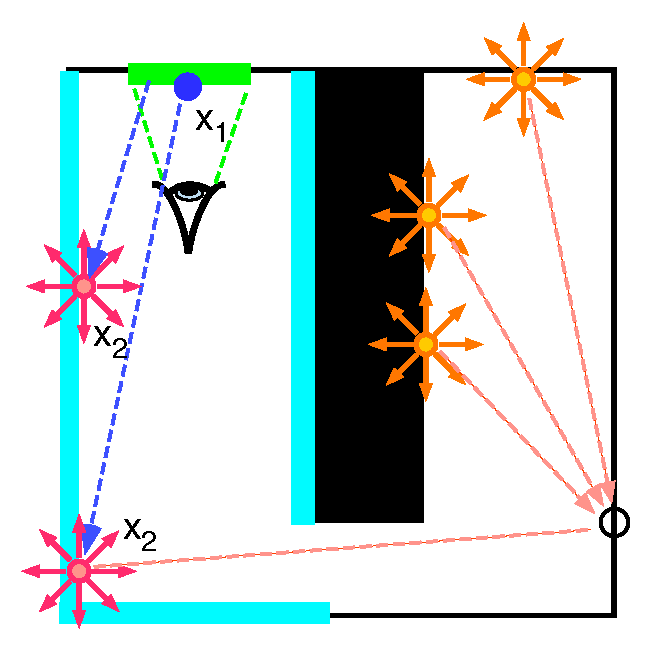
\includegraphics[width=0.55\textwidth]{figures/ir/bir}
	\caption{绿色区域表示摄像机直接可视的区域,也即是着色点$x_1$(蓝色圆点)所在的区域;蓝绿色区域表示能够直接观察到可视区域的区域,也即是反向虚拟点光源$x_2$(红色光源)所在的区域;橙色圆点表示从光源产生的虚拟点光源,通过连接反向虚拟点光源和标准虚拟点光源就产生了反向虚拟点光源的出射辐射亮度场}
	\label{f:ir-bir}
\end{figure}

尽管这里使用了两种方法对虚拟点光源进行采样,但是它们其中的一种采样方法并不是处处都优于或次于另外一种采样方法,例如对于沿摄像机方向的反向采样,图\ref{f:ir-bir}中的蓝绿色区域中只有靠近底部的区域才能有更大概率与标准虚拟点光源相连从而对当前视图形成重大贡献;而对于沿光源方向的正向采样,在图\ref{f:ir-bir}中即便有大部分标准虚拟点光源不能直接照射到可视区域,但是仍然可能会有部分标准虚拟点光源到达左边的蓝绿色区域,从而对当前视图形成重大贡献。

对于上述两种采样方法得到的虚拟点光源样本,如图\ref{f:ir-bir}中的红色和橙色虚拟点光源,我们的目标是要移除那些对当前视图没有任何光照贡献的虚拟点光源,并且使最终虚拟点光源的分布正比于当前视图的重要性分布,因为这样的虚拟点光源样本的方差最低。

然而,我们并没有一个描述虚拟点光源相对于当前视图重要性的概率密度函数,\cite{a:BidirectionalInstantRadiosity}提出可以使用每个虚拟点光源对摄像机的光照贡献来估计它们相对于当前视图的重要性,为此,对于每个虚拟点光源,我们从摄像机均匀发射$M$条长度为2的路径,并且最终的$x-2$顶点落于待估计的虚拟点光源处,我们累加这$M$条摄像机路径的光照贡献作为该虚拟点光源的光照贡献估计,所有虚拟点光源的光照贡献估计就可以建立一个虚拟点光源分布的累积分布函数(cumulative distribution function),该累积分布函数反映了这些虚拟点光源相对于当前视图的重要性。实践上取$M=10$就可以很好地估计该虚拟点光源的重要性分布。

有了当前这些虚拟点光源位置相对于当前视图的重要性分布,这里便可以根据该累积分布函数对当前虚拟点光源进行重采样,那些不重要的区域具有更低的采样概率,这意味着这里可能有一部分虚拟点光源不会被采样而移除掉,减少了虚拟点光源的密度;对于那些光照贡献为0的区域,这里的虚拟点光源会被完全移除掉;而对于那些非常重要的区域,由于采样密度的增加,一些虚拟点光源样本甚至可能被采样多次。最终,通过上述的重采样,最后剩下的虚拟点光源的分布就正比于当前视图的重要性,即每个虚拟点光源样本的光照贡献值为一个常数,从而减少了估计的方差。

上述的方法称为采样/重采样(sampling/resampling)\myindex{采样/重采样}{sampling/resampling}方法,这种方法可行的原因是因为在即时辐射度方法中,第二步光照积分的计算相对于第一步虚拟点光源的生成成本要高(因为每个虚拟点光源对所有像素都产生贡献),我们使用少量($M=10$)的像素样本来估算每个虚拟点光源的光照贡献,从而避免了大量不重要的虚拟点光源最终对所有像素的光照积分计算。此外,通过累加每个虚拟点光源$M$个像素样本的光照贡献,而不是像前面介绍的取舍方法那样对整体所有像素求平均值,这里能够保留每个虚拟点光源比较真实的贡献。

由于场景通常包含大量不能直接观察可视区域的面积,因此实际产生贡献的虚拟点光源相对于整个场景中虚拟点光源的数量要少得多,因此上述的重采样的虚拟点光源的数量通常只是原虚拟点光源很小的一部分,例如只有十分之一,这个比例可以根据场景进行调整。




\subsubsection{虚拟点光源的光照贡献计算}
由于最终是根据每个样本相对于当前视图的重要性进行估计,所以我们需要计算每个样本相对于摄像机的概率密度。

相对于摄像机,每个虚拟点光源的概率密度可以看成是由摄像机发出的一条长度为2的路径$\bar{x}=(x_1,x_2)$的概率密度$p(\bar{x})=p(x_1)p(x_1\to x_2)$,这里$p(x_1\to x_2)$表示从顶点$x_1$处观察到$x_2$的概率规则,设$\mathcal{M}_c$表示所有$x_1$的集合,则根据边缘概率,可以得出:

\begin{equation}
	p(x_2)={\rm \int}_{\mathcal{M}_c}p(x_1)p(x_1\to x_2){\rm d}x_1
\end{equation}

\noindent 如果$x_1$是均匀分布于$\mathcal{M}_c$的,则上式可以简化为:

\begin{equation}
	p(x_2)=\lim_{N\to\infty} \cfrac{1}{N}\sum^{N}_{i_1=1}p(x_{i_1}\to x_2)
\end{equation}

\noindent 因此,我们可以通过发射$M$条摄像机路径的方式来估计每个虚拟点光源的概率密度,这和前面估计光照贡献的原理是类似的,但是这里使用的路径样本数量要大一些,例如\cite{a:BidirectionalInstantRadiosity}使用$M=50$,并且这个数量仅针对标准虚拟点光源,对于反向虚拟点光源,由于它已经位于可以直接观察可视区域的位置,因此使用$M=5$个样本即可以有效地进行估计。

上述的概率密度是每个虚拟点光源在重采样之前的概率密度,由于重采样改变了虚拟点光源的概率密度分布,所以最终上述的概率密度还需要乘以光照贡献累积分布函数的权重,以及每个样本被采样的次数(由于在重采样过程中,每个虚拟点光源可能被采样多次)。

最后, 为了使用蒙特卡洛方法对光照贡献进行计算,除了上述的概率密度函数,每个虚拟点光源还需要知道其辐射亮度分布。对于标准虚拟点光源,它的值已经在(随机行走)传输过程被记录,我们需要注意的是反向虚拟点光源的辐射亮度值。

\cite{a:BidirectionalInstantRadiosity}使用了\cite{a:IlluminationinthePresenceofWeakSingularities}中类似的方法来计算反向虚拟点光源的辐射亮度分布,即首先从反向虚拟点光源处发射多条光线并与场景相交,然后这些交点被当做一个着色点,如图\ref{f:ir-bir}中的黑色圆圈,它们的光照来自于所有标准虚拟点光源。

需要注意的是,由于反向虚拟点光源的出射辐射亮度是根据来自多个方向的光照计算出来的,这不同于标准虚拟点光源只需要记录单个入射辐射亮度值,然后可以根据表面反射系数计算出射辐射亮度分布,因此实际上很难表述反向虚拟点光源的出射辐射亮度分布(或辐射亮度场),所以这里常假设表面为漫反射表面,此时出射辐射亮度场为一个常数。由此可知,双向即时辐射度方法仅适用于漫反射表面,否则需要很高的成本表述反向虚拟点光源的出射辐射亮度分布。




\subsection{梅特波利斯方法}\label{sec:ir-mir}
上述介绍的两种自适应方法本质上都是对已有大量的样本进行再处理,例如舍弃或者重采样(间接地舍弃),通过移除或者重采样操作使最终用于光照计算的虚拟点光源的概率密度正比于当前视图的重要性,因此最终渲染阶段的积分计算的计算量(即参与计算的虚拟点光源的数量)大大减少,提高了即时辐射度方法的效率和质量(因为方差减少了),然而那些被丢弃的样本仍然占据了计算时间。

为了完全避免舍弃或重采样操作,我们需要直接让生成的虚拟点光源的概率密度正比于摄像机的重要性,在本书前面介绍的采样方法中,只有梅特波利斯方法具有使样本的概率密度正比于目标函数的能力,基于此,\cite{a:MetropolisInstantRadiosity}提出了梅特波利斯即时辐射度(Metropolis instant radiosity,MIR)\myindex{梅特波利斯即时辐射度}{Metropolis instant radiosity}方法。除此之外,相对于上述两种方法,MIR方法还具有能够处理复杂可见性场景的能力。

然而,将传统的梅特波利斯光照传输算法(以下简称MLT)直接运用于即时辐射度方法存在很大的困难,这是因为MLT算法产生的样本是一整条路径,而在即时辐射度方法中我们需要知道每条完全路径中顶点$x_2$(即虚拟点光源)处的辐射亮度场以及概率密度,因为最终我们需要将每个虚拟点光源的光照洒向所有像素,而不是像传统的路径追踪算法(如MLT算法那样)那样,每条路径仅对一个像素点产生光照贡献。在MLT算法中,我们通常不需要跟踪每条路径的光照传输,而仅仅是对路径进行累加计数来计算像素的颜色值,这是因为每条路径相对于摄像机的光照贡献均为一个常数,这使得我们没有办法取得每个虚拟点光源$x_2$的辐射亮度场。

尽管如此,MIR算法还是很巧妙地将传统的MLT算法很简单地集成进即时辐射度方法中。和传统的MLT算法一样,首先使用一个普通的(双向)路径追踪得到一个图像的近似估计以消除起始偏差(start-up bias),并得到光照积分的归一化系数$P_c$,即整个图像空间(或者说摄像机)接收到的总能量;然后一个传统的MLT采样过程(可以是本书前面介绍的任意MLT采样方法)被执行,这生成一些概率密度正比于真实光照分布的路径。当然,由于这些路径后面会被运用于即时辐射度方法中,所以这里需要的路径样本数量会远远低于传统MLT算法中路径样本的数量。

接下来,我们需要从这些服从图像真实分布的路径样本中提取出各个虚拟点光源,这包括每个虚拟点光源的出射辐射亮度场,以被后面的即时辐射度积分阶段(即计算每个虚拟点光源对所有像素的光照贡献)使用。这是最困难的部分,按照上面的分析这是不可能得到的信息。\cite{a:BidirectionalInstantRadiosity}指出,尽管我们无法知道每个虚拟点光源确切的辐射亮度场分布,但是我们知道每个虚拟点光源对摄像机(或者说所有像素)总的能量贡献,这是因为整个积分就是关于摄像机接受到的总能量,而MLT算法保证每个路径样本具有相同的能量贡献,因此对于$n$个路径样本,我们可以直接得出每个路径样本对摄像机的能量贡献为$P_c/n$,因此我们也可以得出每个虚拟点光源对摄像机(即所有像素)的能量贡献为$P_c/n$。也就是说,虽然我们不知道每个虚拟点光源的辐射亮度场分布,但是如果我计算该虚拟点光源对所有像素的光照贡献,所有像素接收到该虚拟点光源光照能量的总和应该是$P_c/n$。

如果假设场景全部是漫反射表面,那么虚拟点光源向每个方向发射的能量是相同的,因此每个虚拟点光源的能量$P_c/n$被均匀洒向各个像素,然后我们计算每个像素接收到的光照值,并累加所有像素的光照值为$P^{'}_i$。如果所有像素与虚拟点光源之间不存在遮挡,那么应该存在$p^{'}_i=P_c/n$,然而更常见的情况是部分像素被遮挡,所以这导致$p^{'}_i\neq P_c/n$,这不符合原始MLT算法中每条路径对摄像机的总的光照贡献,所以为了对此进行修正,我们将每个像素得到的光照值乘以一个缩放因子$ \cfrac{P_c}{nP^{'}}$,这就使得所有像素接受到的总能量保持为$P_c/n$。对所有虚拟点光源重复迭代上述的过程,每个像素得到的所有虚拟点光源的累积光照即为最终的图像。

通过上面介绍的机制,我们避免了对每个虚拟点光源出射辐射亮度场的求解,它也是一种无偏的方法,因为我们将每个虚拟点光源的能量正确分配到了每个像素上。然而MIR算法仅仅适用于辐射度设置的场景,因为当虚拟点光源位于光泽表面时,尽管我们可能仍然可以使用某种方法使虚拟点光源对摄像机总的能量贡献保持不变,但是却不能保证每个像素的光照计算是正确的。


\begin{comment}
	


\subsection{连续蒙特卡洛方法}\label{sec:ir-smc-ir}

Nothing is made to ensure temporal coherency
→ if one sample changes, the whole sequence is modified;
Solution: Reuse the previous samples with a sequential sampler (see [GDH06]).

\cite{a:SequentialMonteCarloInstantRadiosity}


\begin{figure}
\begin{fullwidth}
	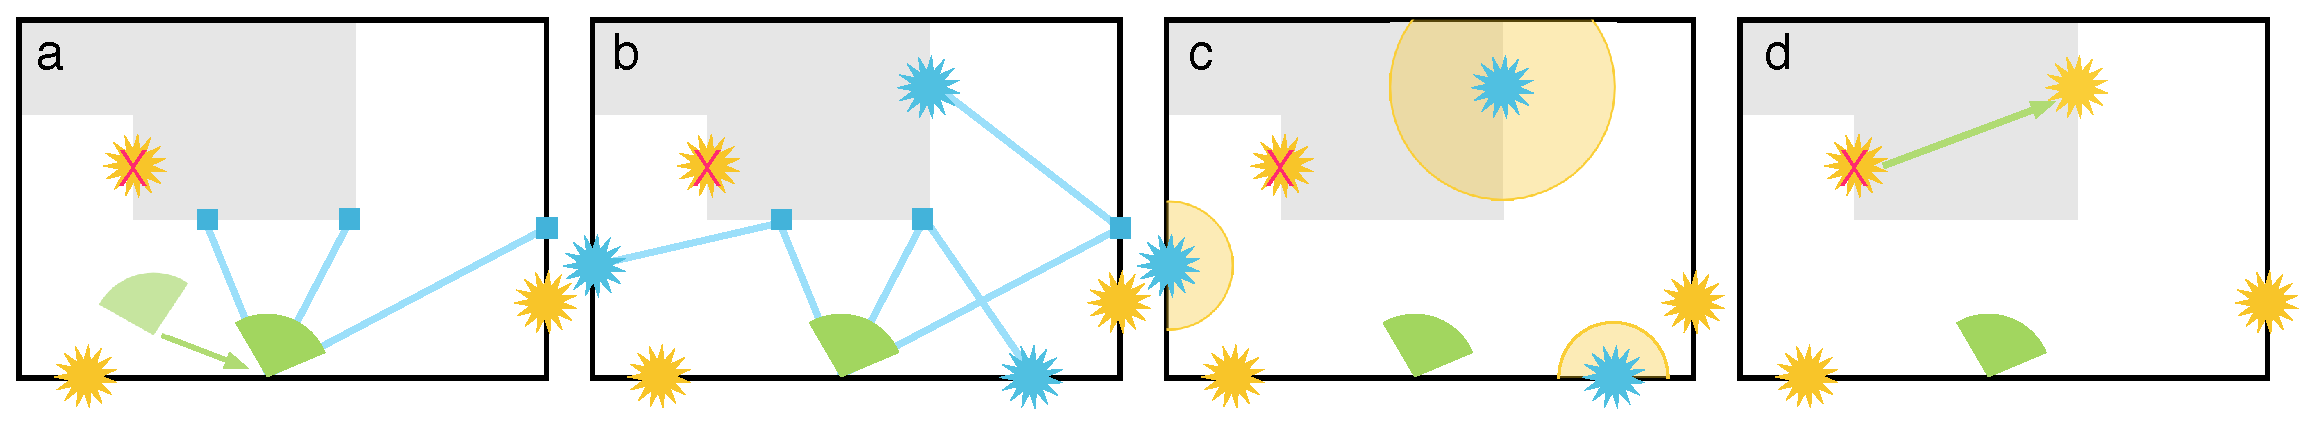
\includegraphics[width=1.0\thewidth]{figures/ir/sequential}
	\caption{ff}
	\label{f:ir-sequential}
\end{fullwidth}
\end{figure}

\end{comment}


\section{偏差补偿}\label{sec:bias-compensation}
本质上,除了光源子路径的每个顶点可以与所有摄像机子路径相连,以及摄像机子路径的长度通常为1,从算法本身来讲,即时辐射度方法和双向路径追踪并无本质上的区别,如果具有足够数量的路径样本,则所有可以被双向路径追踪技术采样的路径仍然可以被即时辐射度方法采样得到,从这个意义上说,即时辐射度方法也是一种无偏方法。

然而,即时辐射度方法被定位为一种高效且高质量的全局光照算法,其高质量来源于它能够处理所有路径的能力,而高效来源于它对渲染方程中被积函数高频分布的限定。在无偏的蒙特卡洛方法中,如路径追踪,高频部分的样本更容易产生较大的方差,因此需要大量的样本来消除这些较高的方差,这也是无偏方法计算成本较高的原因,如果能够将高频部分过滤掉,则低频分布的被积函数可以被数量非常少的样本近似,这便是即时辐射度方法的基本思想。

由于使用了非常少的样本值,被积函数中几何项在距离非常近的情况下会产生奇异值(singularities),如图\ref{f:ir-bias}(a)所示,从而时估计具有较大的方差。在无偏的路径追踪技术中,这种较大的方差可以通过使用更过的样本数量来消除,然而这有违即时辐射度方法的思想,传统的即时辐射度方法\cite{a:InstantRadiosity}通常通过设定一个最小的几何项阈值$b$来限定这种奇异值的产生。

对被积函数函数值的限定,导致了函数的部分值不能被采样,从而导致偏差,因此上述这种限定几何项的方法使即时辐射度方法变为一种有偏估计方法。本节将讨论这种由于对几何项值的限定导致的偏差进行补偿的方法,需要注意的是,偏差补偿不同于偏差减小,后者是通过分析导致偏差的原因从而调整对偏差的影响参数以“减小”偏差,而前者是通过某种方法“找回”丢失的偏差。

\begin{myshaded}
	\indent 即时辐射度方法和光子映射技术中偏差原因的比较。
	
	\indent 虽然同为有偏估计,即时辐射度和光子映射方法中偏差产生的原因并不相同,后者的偏差来源于对样本的平滑(过滤)处理,而这种平滑并不影响对被积函数各个值处的采样;而前者的偏差来源于对被积函数取值的限定(bounding),限定是指将函数的值限制在一定的取值范围,使得高于该阈值的函数值被舍弃掉,从而使这些函数值对应的样本不能被采样而形成偏差。函数值限定在英文文献中有时也使用clampling这个词,该词具有加紧,收缩的意思,但是在图形学上下文中,clamping通常要取限制(而没有挤压)的意思。
	
	\indent 因此,光子映射和即时辐射度方法中减小偏差的方法也是不相同的,前者通过减小核估计的半径来减小偏差,而后者可以通过减少限定阈值来减小偏差。
\end{myshaded}





\subsection{光线追踪方法}
由于即时辐射度方法通常使用非常稀疏的虚拟点光源分布,因此如果某个虚拟点光源和着色点之间的距离比较近时,就会使几何项(由于距离的平方作为分母)出现奇异值,这种奇异值使得如墙角等区域出现非常亮的斑点,如图\ref{chp:ir}(a)所示。在无偏的路径追踪技术中,几何项的奇异值\footnote{其实就是较大的方差,因为这些奇异值与样本的平均值差异较大。}可以通过巨量的样本进行消除,然而由于即时辐射度方法中的虚拟点光源数量非常少,因此无法有效消除。

一个比较简单的方法是对几何项使用一个用户定义的最大限制值$b$,定义以下项为限定几何项(bounded geometry term)\myindex{限定几何项}{bounded geometry term}$G_b(\mathbf{x}\leftrightarrow\mathbf{y})$:

\begin{equation}
	G_b(\mathbf{x}\leftrightarrow\mathbf{y})=\min\{G(\mathbf{x}\leftrightarrow\mathbf{y}),b\}
\end{equation}

\noindent 将上式替换传统的几何项$G(\mathbf{x}\leftrightarrow\mathbf{y})$并代入渲染公式中,就可以消除上述由于近距离几何项的奇异值导致的斑点,形成如图\ref{f:ir-bias}(b)所示的结果。该结果虽然没有了局部凹面位置(如墙角和缝隙等)处的斑点,但是由于丢失了一部分能量(即偏差),这些位置处的光照变得更加黯淡,图\ref{f:ir-bias}(c)显式了无限定和限定条件下光照的差异,即辐射度方法的偏差,本节的主要内容就是要对这部分偏差进行补偿,以形成如图\ref{f:ir-bias}(d)所示的偏差补偿结果。

\begin{figure}
\begin{fullwidth}
	\begin{subfigure}[b]{0.246\thewidth}
		\includegraphics[width=1.0\textwidth]{figures/ir/vpl-noclamping}
		\caption{无限定}
	\end{subfigure}
	\begin{subfigure}[b]{0.246\thewidth}
		\includegraphics[width=1.0\textwidth]{figures/ir/vpl-clamping}
		\caption{限定}
	\end{subfigure}
	\begin{subfigure}[b]{0.246\thewidth}
		\includegraphics[width=1.0\textwidth]{figures/ir/vpl-difference4x}
		\caption{偏差 = (a) - (b)}
	\end{subfigure}
	\begin{subfigure}[b]{0.246\thewidth}
		\includegraphics[width=1.0\textwidth]{figures/ir/vpl-compensated}
		\caption{偏差补偿}
	\end{subfigure}
	\caption{即时辐射度方法通常使用数量非常少的路径样本,因此由于近距离几何项导致的高方差无法通过样本数量的增加进行收敛,这形成如图(a)所示的斑点,这种奇异值可以简单地通过限定几何项的最大值进行消除(b),然而由于限定丢失了能量,这使得被限定的几何位置光照更找黯淡,无限定和限定光照的偏差(c)可以通过本节介绍的方法进行补偿(d)(图片来自\cite{u:VirtualPointLightBiasCompensation})}
	\label{f:ir-bias}
\end{fullwidth}
\end{figure}

由于几何项的限定,原始的被积函数丢失了部分能量,为了对偏差进行补偿,我们需要首先对这部分偏差进行描述。这里首先定义一个残留几何项(residual geometry term)\myindex{残留几何项}{residual geometry term}$G_r(\mathbf{x}\leftrightarrow\mathbf{y})$用于传输丢失的能量:

\begin{equation}
\begin{aligned}
	G_r(\mathbf{x}\leftrightarrow\mathbf{y})=&G(\mathbf{x}\leftrightarrow\mathbf{y})-G_b(\mathbf{x}\leftrightarrow\mathbf{y})\\
	=&G(\mathbf{x}\leftrightarrow\mathbf{y})-\min\{G(\mathbf{x}\leftrightarrow\mathbf{y}),b\}\\
	=&\max\{G(\mathbf{x}\leftrightarrow\mathbf{y})-b,0\}
\end{aligned}
\end{equation}

本质上,限定几何项和残留几何项只是将原始几何项按值域划分成了两个不同的部分,其中并不包含什么特别的处理方式,在数学形式上它们是完全等效的,这种划分最后表现为对表面上区域的一种划分,例如离$\mathbf{x}$较近的点$\mathbf{y}$可能属于残留几何项,而较远的点$\mathbf{y}$则属于限定几何项。

既然它们的数学形式是完全相同的,那么它们各自对应的光照贡献值应该也是可以按照相同的方式进行计算的。例如对于限定几何项,每个着色点$\mathbf{x}$的颜色值来自于场景中所有位于限定几何区域的虚拟点光源的直接光照;理论上,我们可以将这种方式推广到残留几何区域,然而这种直接的推广却遇到困难:因为残留几何区域非常小,同时由于虚拟点光源的分布非常稀疏,所以残留几何区域完全可能不存在任何虚拟点光源(从图\ref{f:ir-bias}(a)中可以看到残留几何区域的虚拟点光源分布非常稀疏),因而上述的方法无法计算光照偏差。

这就使得我们必须寻求另一种方法来计算残留几何区域的光照。从渲染方程本身来看,每个点的辐射亮度等于该点半球面上所有入射辐射亮度的积分,对于限定几何项,由于其范围较大,因此场景中所有的虚拟点光源的方向能够覆盖大部分半球面空间,所以使用虚拟点光源的光照作为入射辐射亮度就足够估计其光照;然而对于残留几何区域,虚拟点光源不足以覆盖整个半球面空间,所以\cite{a:IlluminationinthePresenceofWeakSingularities}将残留几何项对应的光照贡献的计算退回到传统的光线追踪方法中:虽然半球空间残留几何区域内可能不包含任何虚拟点光源,但是我们只要求出这些方向上的入射辐射亮度即可,它们可以通过光线追踪的方式进行计算,这种方法成为了后面即时辐射度方法偏差补偿的重要基础。

为此,我们首先需要将传统的基于表面位置(即虚拟点光源的位置)的光照积分形式改为基于方向的积分形式,这些方向对应的表面顶点由光线投射$h(x,\omega)$计算,例如如下的残留光照贡献:

\begin{equation}
\begin{aligned}
	&L(x,\omega_r)-L_b(x,\omega_r)\\
	&={\rm \int}_AL_e(y,-\omega)f_r(\omega,x,\omega_r)V(x,y)\max\{G(x,y)-b,0\}dy\\
	&={\rm \int}_AL_e(y,-\omega)f_r(\omega,x,\omega_r)V(x,y) \cfrac{\max\{G(x,y)-b,0\}}{G(x,y)}G(x,y) {\rm d}y\\
	&={\rm \int}_{S^{2}}L_e(h(x,\omega),-\omega) \cfrac{\max\{G(x,h(x,\omega))-b,0\}}{G(x,h(x,\omega))}f_r(\omega,x,\omega_r)\cos\theta_x {\rm d}\omega
\end{aligned}
\end{equation}

\noindent 其中,$L_b(x,\omega_r)$表示限定几何区域的光照贡献,最大值函数$\max\{G(x,h(x,\omega))-b,0\}$将光线方向限定在了残留几何区域,这里可以使用密度函数$f_r(\omega,x,\omega_r)\cos\theta_x$对方向进行重要性采样。

与传统的光线追踪算法相比,这里的残留几何区域面积非常小,所以其计算成本相对非常低,并且由光线投射决定的点$y=h(x,\omega)$的光照仍然是使用虚拟点光源进行估计,因此进一步降低残留光照的计算量。

\begin{figure}
\begin{fullwidth}
	\includegraphics[width=1.0\thewidth]{figures/ir/bias-compensation}
	\caption{对于着色顶点$x_1$,它的光照可以分为两部分,其中红色的箭头表示来自限定几何区域内虚拟点光源的直接光照,而紫色箭头表示来自残留几何区域内虚拟点光源的光照,由于残留几何区域内的虚拟点光源数量非常少,因此我们使用光线追踪的方法来计算这部分的光照,这里蓝色箭头表示摄像机子路径,由着色点$x_1$向残留几何区域发射光线产生补偿顶点$x_2$,然后将顶点$x_2$看做一个着色顶点继续上述的计算,这样的过程不断迭代(例如产生补偿顶点$x_3$),直到满足终止条件}
	\label{f:ir-bias-compensation}
\end{fullwidth}
\end{figure}

图\ref{f:ir-bias-compensation}显式了残留光照的计算过程,$x_1$为着色点,红色箭头表示来自限定区域内($G_b(x_1\leftrightarrow x^{i}_2)<b$)虚拟点光源的光照,它们通过传统的即时辐射度方法进行计算;而紫色箭头表示来自残留区域内($G(x_1\leftrightarrow x^{i}_2)>b$)虚拟点光源的光照,这部分光照由于虚拟点光源的数量非常少,因此我们使用传统的光线追踪计算残留几何区域的光照,如图\ref{f:ir-bias-compensation}中间小图所示,通过对$x_1$的半球面进行方向采样得到位于残留几何区域内的点$x_2$,$x_2$又称为补偿顶点(compensation vertex)\myindex{补偿顶点}{compensation vertex},为了得出点$x_2$向$x_1$方向的辐射亮度,我们把$x_1$当做观察点,把点$x_2$当做一个着色顶点,然后重复上述的过程计算顶点$x_2$的光照,例如顶点$x_2$的一部分光照来自限定几何区域的虚拟点光源,而另一部分来自于残留几何区域内虚拟点光源的光照,同样由于残留几何区域内虚拟点光源的密度很低,因此顶点$x_2$的残留光照仍然通过偏差补偿的方式进行计算。上述的过程不断迭代下去,直到满足一定的终止条件(例如对光线的反射或吸收使用俄罗斯轮盘进行采样)。

由于补偿顶点$x_2$的光照计算仍然包含偏差补偿项,因此上述的偏差补偿方法是一个迭代方法。尽管残留光照被使用了传统的光线追踪进行计算,但是光线投射的范围仅仅被限定在了很小的局部区域,因此计算成本较原始的光线追踪非常小,并且每个补偿顶点的光照仍然使用虚拟点光源进行计算,光线的密度分布非常低。

很容易看出,上述的偏差补偿方法是一种无偏方法:所以计算都完全依赖于虚拟点光源和直接光源的光照,并且由于即时辐射度方法具有对所有路径进行采样的能力,只要虚拟点光源的数量足够多,最终图像能够收敛到正确结果,因此其整个迭代估计是无偏的。

尽管如此,上述基于光线追踪的偏差补偿方法仍然很难满足交互性甚至实时的需求,因为随着迭代的不断深入,偏差补偿部分的算法退化为传统的分布式光线追踪,它的计算成本呈数量级增长。



\subsubsection{参与介质中的近似方法}
\cite{a:UnbiasedGlobalIlluminationwithParticipatingMedia}将即时辐射度方法以及上述的偏差补偿引入到参与介质中,相较于传统的即时辐射度方法,其唯一的区别就是虚拟点光源分布于参与介质内部的各个位置(而不仅仅是表面)处。

然而相较于表面的情况,参与介质的情况要复杂一些,在表面中,由于虚拟点光源与附近的着色点具有相同方向的法线,它们之间并不能形成直接光照,着色点仅接受来自其他具有不同法线方向的虚拟点光源的光照,因此由于几何项导致的奇异值斑点仅出现于凹面墙角处的位置,如图\ref{f:ir-bias}(a)所示;但是因为散射发生于参与介质内部的各个位置,虚拟点光源对所有附近的着色点都会形成单调几何项值,所以几何项导致的奇异值斑点会更加明显,如图\ref{f:ir-unbounded-media}所示,所以参与介质中的偏差补偿需要更加高效的方法。

\begin{figure}
	\sidecaption
	\includegraphics[width=0.35\textwidth]{figures/ir/unbounded-media}
	\caption{在物体表面,即时辐射度方法的单调斑点仅出现于凹面墙角处,因为虚拟点光源对处于同一平面内的着色点并没有光照贡献;但是在参与介质中,虚拟点光源对其附近的任意着色点都有光照贡献,所以单调斑点在参与介质中的现象会更加严重}
	\label{f:ir-unbounded-media}
\end{figure}

通过分析参与介质以及偏差补偿的一些特点,\cite{a:ApproximateBiasCompensationforRenderingSceneswithHeterogeneousParticipatingMedia}提出了一种基于传统偏差补偿的方法,称为近似偏差补偿(approximate bias compensation,ABC)\myindex{近似偏差补偿}{approximate bias compensation},该方法基于一些优化,采样策略以及简化,以下我们分别简要介绍。



\paragraph{限制迭代深度}
在前面介绍的基于光线追踪的偏差补偿方法中,因为补偿顶点的光照仍然包含着限定,因此偏差补偿光照中仍然包含着偏差,因此偏差补偿是一个迭代的过程。但是,由于偏差补偿光照是辐射亮度和BRDF反射函数的卷积,因此偏差补偿的光照随着迭代深度的递增而呈指数递减,并且参与介质中到处都会吸收光照,所以通常$2~3$个迭代就能达到接近真实的结果。



\paragraph{假设局部同质}
对于补偿顶点的生成,我们的目标是通过光线投射在残留几何区域内得到一个顶点,然而在异质介质中,我们无法通过一个给定的距离值对透射比函数进行采样得到一个顶点位置。为了使用光线投射得到补偿顶点,传统的方法(如\cite{a:UnbiasedGlobalIlluminationwithParticipatingMedia})选择一个随机的方向并使用伍德科克跟踪(Woodcock tracking)来得到一个距离采样,如果该距离超出残留几何区域则会被拒绝,这种方法增加了偏差补偿估计的方差,并且增加了计算成本。

如果假设着色顶点的局部范围内是同质的,则上述的补偿顶点采样问题可以被更高效的处理。此时,该局部区域可以使用几何限定阈值$b$表述为一个球面空间,其半径为$d=1/\sqrt{{b}}$,其消光系数为该区域内的平均消光系数$\bar{\sigma}_t$,则以$y$为中心,在半径$d$的球面空间内距离为$t$的概率密度函数为:

\begin{equation}
	p(t)= \cfrac{\bar{\sigma}_t {\rm e}^{-\bar{\sigma}_t}}{1-{\rm e}^{-\bar{\sigma}_t d}}
\end{equation}

\noindent 使用逆变换采样方法得到的距离为:

\begin{equation}
	t=- \cfrac{\ln(1-\xi(1-{\rm e}^{\bar{\sigma}_td}))}{\bar{\sigma}_t}
\end{equation}

\noindent 这里$\xi\in[0,1)$是一个均匀分布的随机数。

尽管这里使用了局部同质的假设,但是这个假设并不影响最终的计算结果,因为它只是用来得到一个补偿顶点的采样位置,最终每个补偿顶点的光照还是根据使用正确的透射比$\uptau(y,y^{'})$进行计算的\footnote{出于效率原因,\cite{a:ApproximateBiasCompensationforRenderingSceneswithHeterogeneousParticipatingMedia}仍然使用了一个近似方法来计算透射比:$\uptau(y,y^{'})=\exp(-\bar{\sigma}_t||y-y^{'}||)$。}。局部同质的假设使得可以直接在残留几何区域内的空间中进行采样,而不需要使用如伍德科克跟踪一样的取舍算法。



\paragraph{积分策略}
在原始的偏差补偿方法中,每个着色点通过光线投射产生多个补偿顶点,然后每个顶点接受来自所有虚拟点光源的光照,这就要求所有虚拟点光源的阴影图等信息随时处于内存中,这样的积分策略对图形硬件的架构不是很友好。

为了充分利用图形硬件的计算效率,\cite{a:ApproximateBiasCompensationforRenderingSceneswithHeterogeneousParticipatingMedia}提出了一种称为1对1的方法,在该方法中,每个摄像机光线上处于介质中的部分产生多个着色顶点,每个着色点只产生一个补偿顶点,每个补偿顶点每次只连接一个虚拟点光源,这样就可以并行处理多个补偿顶点,并且可以每次只处理一个虚拟点光源,因此内存中只需要存储一个虚拟点光源的阴影图。

\begin{figure}
	\sidecaption
	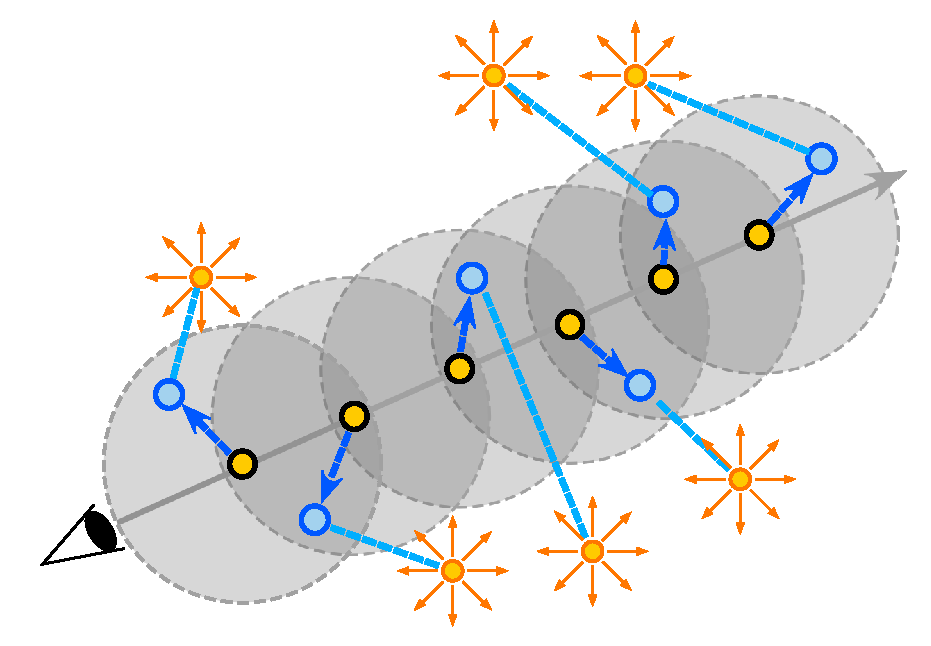
\includegraphics[width=0.5\textwidth]{figures/ir/connection-strategies}
	\caption{为了充分利用图形处理器的计算能力,这里每次对每个着色顶点只生产一个补偿顶点,然后每个补偿顶点每次只接受一个虚拟点光源的光照,这样就可以使用图形处理器并行地对补偿顶点近似计算}
	\label{f:connection-strategies}
\end{figure}



\paragraph{忽略局部可见性}
在传统的偏差补偿中,补偿顶点是由光线投射产生的,而光线投射的过程包含了可见性计算,这也是非常耗费时间的计算过程。但是本节讨论的近似方法是首先(使用非光线投射的方法)确定出一个补偿顶点的位置,这个过程的计算成本几乎是可以忽略的,但是为了计算补偿顶点对着色顶点的光照贡献,我们还是需要确定着色顶点到补偿顶点之间的可见性。然而\cite{a:ApproximateBiasCompensationforRenderingSceneswithHeterogeneousParticipatingMedia}发现,在参与介质中,通过忽略局部残留几何区域内的可见性,往往仍然可以得到非常高质量的结果,这种差异以至于人眼很难察觉。




\subsection{屏幕空间方法}
前面讨论的偏差补偿方法都是基于物体空间(object-space)的,尽管光线追踪部分被限定至一个很小的局部区域,但是由于偏差补偿的迭代特性,偏差补偿光照的计算很快退化至传统的分布式光线追踪,使得其很难达到交互式甚至实时的需求,而这往往正是即时辐射度方法的目标。

传统偏差补偿方法中的瓶颈主要来自于光线投射过程,这需要在物体空间执行成本比较高的光线-物体相交测试。由于偏差补偿中的光线投射只作用与离光线起点较近的环境,而观察到大部分近距离的表面所有的信息都可以从屏幕空间获得,\cite{a:Screen-SpaceBiasCompensationfor}提出了一种对GPU友好的基于屏幕空间的偏差补偿(screen-space bias compensation,SSBC)\myindex{屏幕空间偏差补偿}{screen-space bias compensation}方法,该方法使用一个后处理的过程执行偏差补偿,可以以交互式的速度达到媲美离线算法的结果。




\subsubsection{残留传输操作符}
在前面介绍的基于光线追踪的偏差补偿方法中,对于每一个着色点,它需要计算该着色点对应的所有补偿顶点的入射光照以决定这些补偿顶点对该着色顶点的光照,因此,即使相邻两个着色顶点拥有一个共同位置处的补偿顶点(可以认为是同一补偿顶点),该补偿顶点不得不对每个着色顶点分别计算一次入射光照的积分计算。这种重复计算的特征是由于该偏差算法的迭代公式决定的,基于此观察,\cite{a:Screen-SpaceBiasCompensationfor}对偏差补偿使用了一个新的公式形式,避免了这种重复计算,提高了计算效率。

首先,这里定义一个残留传输操作符(residual operator)\myindex{残留传输操作符}{residual operator}用于表述限定和非限定传输操作符的差:即$\mathbf{T}_r = \mathbf{T}-\mathbf{T}_b$,将这些新的传输操作符\footnote{
注意,这些传输操作符的不同点仅在于几何项,例如:

\begin{equation*}
\begin{aligned}
	\mathbf{T}\hat{L}  &=\sum^{N}_{i=1}f_rGV\hat{L}\\
	\mathbf{T}_b\hat{L}&=\sum^{N}_{i=1}f_r \min(G,b)V\hat{L}\\
	\mathbf{T}_r\hat{L}&=\sum^{N}_{i=1}f_r \max(G-b,0)V\hat{L}
\end{aligned}
\end{equation*}

这里$b$表示用户定义的几何项限制阈值,它们的作用结果如图\ref{f:ir-residual-operator}(a),(c)和(d)所示。 
}代入到以传输操作符表述的渲染公式中得到:

\begin{equation}
	L=L_e+\mathbf{T}L_e+\mathbf{T}_b\hat{L}+\mathbf{T}_r\hat{L}
\end{equation}

\noindent 这里$(\hat{L})$表示所有来自于虚拟点光源的间接光照,从上式可以看出,将限定传输操作符$\mathbf{T}_b$作用于$(\hat{L})$并不会导致奇异值,这也正是对即时辐射度方法使用限定的原因,但是将残留传输操作符$\mathbf{T}_r$作用于$\hat{L}$却会遭受奇异值。

为了推导出一种新的偏差补偿技术,考虑到$\hat{L}$表述的是间接光照,它表示场景中处自发光之外的的真实光照,即$\hat{L}=L-L_e$,所以我们可以将导致奇异值的间接光照替换为一般的真实间接光照$\hat{L}=L-L_e$,由于不再使用虚拟点光源进行近似,所以残留操作符$\mathbf{T}_r$的奇异值消失了\footnote{正是由于虚拟点光源的近似和样本的不足,才导致了奇异值斑点,而真实光照包含了无偏的结果,残留传输操作符作用于该光照并不会产生奇异值。}。 通过这样的调整,渲染方程的结果保持不变,其唯一的变化是残留传输操作符现在作用于真实反射光照(而不是来自虚拟点光源的光照),如图\ref{f:ir-residual-operator}(b),(c)和(e)所示:

\begin{equation}
	L=L_e+\mathbf{T}L_e+\mathbf{T}_b\hat{L}+\mathbf{T}_r(L-L_e)
\end{equation}

\noindent 然而实际上我们并不知道上述的真实光照$L$,上式右式的结果同时出现于右式中,通过递归地展开,可以得到一个针对即时辐射度的新的无偏估计公式:

\begin{equation}\label{e:ir-ssbc}
	L=L_e+\sum^{\infty}_{i=0}\mathbf{T}^{i}_r(\mathbf{T}L_e+\mathbf{T}_b\hat{L})
\end{equation}

\noindent 注意这里$\mathbf{T}_b\hat{L}$是无偏的,上式说明我们可以通过将残留传输操作符递归地作用于直接和限定间接光照来得到一个无偏的估计。上式右边和式中的第一项表示直接和限定间接光照,它们合称为限定贡献值(clamped contribution)\myindex{限定贡献值}{clamped contribution},每深入一级的加和表示上一级限定贡献值的限定补偿(clamped compensation)\myindex{限定补偿}{clamped compensation}。并且式\ref{e:ir-ssbc}说明,在整个偏差补偿过程中,我们只需要对直接光照$\mathbf{T}L_e$和虚拟点光源的限定光照$\mathbf{T}_b\hat{L}$计算一次。

\begin{figure}
\begin{fullwidth}
	\begin{subfigure}[b]{0.195\thewidth}
		\includegraphics[width=1.0\textwidth]{figures/ir/ir-7-1}
		\caption{= (c) + (d)}
	\end{subfigure}
	\begin{subfigure}[b]{0.195\thewidth}
		\includegraphics[width=1.0\textwidth]{figures/ir/ir-7-4}
		\caption{= (c) + (e)}
	\end{subfigure}
	\begin{subfigure}[b]{0.195\thewidth}
		\includegraphics[width=1.0\textwidth]{figures/ir/ir-7-2}
		\caption{$L_e+\mathbf{T}L_e+\mathbf{T}_b\hat{L}$}
	\end{subfigure}
	\begin{subfigure}[b]{0.195\thewidth}
		\includegraphics[width=1.0\textwidth]{figures/ir/ir-7-3}
		\caption{$\mathbf{T}_r\hat{L}$}
	\end{subfigure}
	\begin{subfigure}[b]{0.195\thewidth}
		\includegraphics[width=1.0\textwidth]{figures/ir/ir-7-6}
		\caption{$\mathbf{T}_r(L-L_e)$}
	\end{subfigure}
\caption{限定和残留光照传输,注意:因为残留传输操作符$\mathbf{T}_r$作用于虚拟点光源产生的间接光照$\hat{L}$时会遭受奇异值,所以(a)中包含这奇异值斑点;但是(b)确实无偏的,因为它移除了会产生奇异值的$\hat{L}$,而使用一个真实的反射光照$L-L_e$代替(图片来自\cite{a:Screen-SpaceBiasCompensationfor})}
\label{f:ir-residual-operator}
\end{fullwidth}
\end{figure}

通过式\ref{e:ir-ssbc}可以得出一个很重要的观察,因为由于补偿得到的光照等于光源与BRDF分布函数执行$N+1$次卷积的结果,所以它随着$N$的增加呈指数式下降,由于漫反射表面具有较低的反射率,所以实践上通常少数几次(如1至3次)迭代就可以得到与无偏方法相媲美的结果。

根据式\ref{e:ir-ssbc}的渲染公式形式,\cite{a:Screen-SpaceBiasCompensationfor}提出一个新的偏差补偿算法,它包含两个主要步骤:

\begin{enumerate}
	\item 首先,每个着色点的第一级限定段贡献值被计算,这包含将传输操作符$\mathbf{T}$作用于光源的直接光照,以及将限定传输操作符$\mathbf{T}_b$作用于虚拟点光源的限定间接光照。
	\item 其次,将残留操作符$\mathbf{T}_r$作用于上述的限定贡献值,并依次迭代$N$次以计算上述限定贡献值的补偿。
\end{enumerate}

与前面基于物体空间的偏差补偿方法不同的是,SSBC仅计算屏幕空间的着色点,并且仅仅使用这些着色点来补偿偏差(注意,基于光线追踪的偏差补偿是使用整体物体空间的表面来补偿偏差)。这使得SSBC具有两个优势:首先,它可以以后处理的方式将残留传输操作符仅作用于屏幕空间的着色点上;其次,它可以很容易地找出那些对着色点的偏差补偿具有潜在贡献的表面顶点,因为那些在物体空间相邻的顶点往往也相邻于屏幕空间。

以下我们详细讨论这种基于屏幕空间的偏差补偿技术。




\subsubsection{屏幕空间的积分}
光照传输操作符(包括$\mathbf{T}_r$)可以表述为围绕表面的积分,对$\mathbf{T}_r$执行屏幕空间的近似计算意味着将该针对表面的积分形式转化为针对有限个像素的和的形式。对于每一个像素,我们可以在后处理阶段从G-buffer中提取每个像素的位置$\mathbf{z}_i$,法线$\mathbf{n}_i$,并可以通过屏幕空间的投影关系计算出每个像素在世界空间的面积$A_i$。

因此,对于一个着色点$\mathbf{y}$,其来自附近$M$个像素的残留光照传输为:

\begin{equation}\label{e:ir-operator}
	\mathbf{T}_r\hat{L}\approx\sum^{M}_{i=1}f_r(x\leftarrow y\leftarrow z_i)G_r(y\leftrightarrow z_i)V(y\leftrightarrow z_i)L(y\leftrightarrow z_i)A_i
\end{equation}

\noindent 正如前面提到的,只要那些靠近着色点$y$的表面才会对其偏差补偿形成贡献,其他位置的残留几何项则为$G_r(y\leftrightarrow z_i)=0$。我们可以基于限定几何项$G_b$的限定值$b$计算出一个球面包围区域,该球面在世界空间的半径为$r=1/\sqrt{b}$,如图\ref{f:ir-ssbc}(b)所示,该区域包含所有能够对着色点的偏差形成贡献的补偿顶点。我们可以很容易地将该世界空间的半径距离转化到屏幕空间,例如对于透视投影,$r_s=r/(tan(\delta /2)||x-y||)$,这里$\delta$表示视场角。

\begin{figure}
\begin{fullwidth}	
	\includegraphics[width=1.0\thewidth]{figures/ir/ir-6-1}
	\caption{SSBC通过将残留传输操作符(根据视图方向)适应性地运用于屏幕空间的像素来计算偏差补偿(a),为了寻找补偿顶点,首先对每个着色点计算出一个包含所有补偿顶点的限定区域(b),该区域内的所有像素都是对着色点的偏差补偿产生贡献的补偿像素,更进一步,G-buffer被组织为一个阶层式的结构以提升计算性能(c)和(d),跨越非连续边界或占据较大投影立体角的像素被进一步细化(R),直到它们的贡献能够被精确表述($1$),或者该像素被完全丢弃($0$),每个像素执行偏差补偿的样本数量如(e)所示(图片来自\cite{a:Screen-SpaceBiasCompensationfor})}
	\label{f:ir-ssbc}
\end{fullwidth}
\end{figure}

通过这种限定区域由世界空间到屏幕空间的转换,我们就把一个基于表面的积分转换为一个基于屏幕像素的和式形式,并把和式的像素范围限制在了屏幕区域,此外SSBC忽略了局部像素之间的可见性。

需要注意的是,屏幕空间的半径距离$r_s$依赖于着色点$y$距离摄像机的距离,对于里摄像机较近的着色点$y$,其包围球面的半径变得更大因此覆盖更多的像素,所以下面提出一个阶层式的结构用于提升计算补偿光照的性能。 



\subsubsection{阶层式积分}
屏幕空间阶层式积分的目标是对那些较远(但仍处于限定区域内)的表面使用更少的像素样本,图\ref{f:ir-ssbc}演示了这种针对当前视图的适应性采样,以及当光照表述不够精确时的进一步细化。

为了实现阶层式积分,这里首先对G-buffer计算出一个多级纹理,每个纹素的值包括像素的位置,法线,材质属性,累加的像素面积,以及反射的限定光照。同时这里还使用了一个类似于\cite{a:Hierarchicalimage-spaceradiosityforinteractiveglobalillumination}的非连续缓冲区用于存储表面的非连续边界,该缓冲区也以多级纹理表述,它们被用来避免对非连续边界或深度不连续的区域执行积分计算。

当开始计算表面对着色点的偏差补偿贡献时,我们首先从最粗糙的多级纹理开始,并决定该级纹理对着色点的偏差光照贡献是否足够精确,否则就是要更精细的多级纹理来计算对着色点的偏差补偿。为了避免空间和时间上的失真,这里使用两个细化标准:

\begin{enumerate}
	\item 补偿像素对应的表面到着色点的投影立体角超过一定的阈值(通常为0.08sr),因为当投影立体角比较大时,这通常意味着表面本身面积比较大,或者表面更加靠近着色点$y$,因此需要更精细的偏差补偿光照计算。
	\item 当前的样本跨越了一个非连续边界,此时粗糙的多级纹理中的位置,法线和面积都不能正确地表述原始的几何特征。
\end{enumerate}

只要满足上述两个细节标准中的任意一个,就忽略当前的多级纹理,而使用下一个更加精细的级别,这通过对当前像素在下一级纹理中周围相邻4个像素进行加和来实现。当然,上述的第二个细化标准可能会导致一些不重要的区域(例如那些较远的表面)被使用了过多的细化,所以通常只有那些投影固体的超过一定阈值($\approx 0.04$)的表面才会根据非连续边界执行细化。

图\ref{f:ir-ssbc}(c)和(d)显式了对补偿顶点执行细化的过程,其中R表示需要细化的像素,1表示对偏差补偿具有贡献(同时不需要细化)的像素,而0表示对着色点的偏差补偿没有贡献的像素。
 
最后简要总结一下SSBC算法的过程。首先,在预处理阶段,我们使用传统的即时辐射度方法计算出每个像素(着色点)的限定光照贡献(包含直接和来自虚拟点光源的限定光照贡献,即$\mathbf{T}L_e+\mathbf{T}_b\hat{L}$),这些限定光照值连同像素的位置,法线等信息被存储在G-buffer中被后处理的SSBC算法使用。本质上,具有非零值限定光照贡献的像素都是需要执行偏差补偿的像素,每次迭代中的限定光照贡献都被累加到最终的图像缓冲区上,它表示的是上一次迭代中限定光照贡献的补偿光照贡献值。

然后,后处理阶段使用一个计算着色器来处理上一次迭代的偏差补偿,计算着色器将存储位置,法线,像素面积,表面BRDF,以及限定光照贡献值的多级G-buffer作为输入,并对所有具有非零限定光照值的像素执行偏差补偿计算,它首先将这些像素点视作为着色点寻找对其偏差补偿产生贡献的邻近像素,即补偿顶点,然后计算这些补偿顶点对该“着色点”的光照贡献,这个过程涉及对阶层的细化选择,其计算出的光照贡献作为该次迭代的限定光照贡献,每次迭代中的限定光照贡献表示上一次迭代的补偿光照贡献,并且这些限定光照贡献值作为下一次迭代的输入以计算该次限定光照的补偿光照,以此迭代下去,直到满足终止条件。

需要注意的是,在计算邻近的补偿像素对着色像素的光照贡献时,实际上计算的是一个补偿像素在世界空间对应的面积对着色像素在世界空间的面积的光照,这需要在辐射度设置下进行计算,因此SSBC比较适用于漫反射表面(在本章后面我们还会继续讨论使用于光泽表面的偏差补偿方法),否则偏差补偿的计算将变得比较复杂。




\section{避免奇异值——光泽表面的处理}
通过前面的内容可知,即时辐射度使用了远少于路径追踪算法的路径样本。虽然较少的路径样本意味着较高的估计方差,但是即时辐射度方法通过将每个光源子路径重用于所有着色点,这样每个虚拟点光源都能够对整个场景形成贡献,使得图像分布更加平滑,不会像路径追踪那样表现为刺眼的噪点,达到交互式的能力。

\begin{figure}
\begin{fullwidth}
	\begin{subfigure}[b]{0.33\thewidth}
		\includegraphics[width=1.0\textwidth]{figures/ir/vsl-glossy-spikes}
		\caption{光泽反射斑点}
	\end{subfigure}
	\begin{subfigure}[b]{0.33\thewidth}
		\includegraphics[width=1.0\textwidth]{figures/ir/vsl-g-spikes}
		\caption{几何项斑点}
	\end{subfigure}
	\begin{subfigure}[b]{0.33\thewidth}
		\includegraphics[width=1.0\textwidth]{figures/ir/vsl-reference}
		\caption{参考图像}
	\end{subfigure}
	\caption{即时辐射度方法由于仅使用了少量的路径样本,所以那些高频部分的函数值往往表现为奇异值,这在渲染结果中表现为白色斑点,这些斑点通常有两种来源,即由于光泽或镜面反射产生的强烈光照(a),它们往往分布于光泽反射方向上的表面;以及来自相邻两个顶点产生的几何项值(b),它们往往分布于墙角等凹面位置处(图片来自\cite{a:VirtualSphericalGaussianLightsforRealtimeGlossyIndirectIllumination})}
	\label{f:ir-avoid-singularities}
\end{fullwidth}
\end{figure}

尽管如此,光照分布函数的高频部分始终是需要更多的样本才能达到足够的近似。在渲染方程中,有两个因素会使得光照分布函数的频率变化非常高,首先是光泽或镜面表面的反射光照,其次是非常靠近的两个相邻顶点形成的几何项值,它们在虚拟点光源数量不足的即时辐射度算法中的效果如图\ref{f:ir-avoid-singularities}(a)所示,在样本非常稀疏的即时辐射度方法中,高频部分往往表现为奇异值,这些奇异值在即时辐射度方法中导致白色的光斑。在本章到目前为止的内容中,我们往往将即时辐射度方法限定于漫反射表面,这使得光斑仅仅分布于墙角等凹面位置处,如图\ref{f:ir-avoid-singularities}(b)所示,这些由于几何项限定导致的偏差可以进一步被一些偏差补偿技术进行补偿。

\begin{myshaded}
	\indent 即时辐射度方法中的光斑与路径追踪中的噪点:
	
	\indent 在路径追踪技术中,当样本数量不足时,其方差往往表现为单个噪点,这是因为每个路径样本都作用于单个着色点;然而在即时辐射度方法中,每个虚拟点光源作用于所有着色点,即单个奇异值的光照被分配多个着色点上,所以它表现为一个不那么刺眼的斑点,例如对于一个光泽表面的虚拟点光源,它的光照大部分被反射至一个很小的表面上,形成小小的光斑,并且由于光泽BRDF并不是一个常数,因为光斑的边缘呈现一种从1到0的过度,没有单个着色点的噪点那么刺眼。
	
	\indent 但是光斑的这种平滑的效果并不意味着其方差更小,方差跟图像的视觉表现并没有关系,它仅仅与样本的平均值有关,即时辐射度方法中的斑点和路径追踪中的噪点本质上都是方差的视觉表现。即时辐射度这种视觉“悦眼”程度是因为它的每个光源子路径与所有摄像机子路径相连,路径的相连需要执行可见性计算,其成本非常大,而即时辐射度方法正是利用图形硬件的光栅化能力来执行这种大量的可见性测试。
\end{myshaded}

在后续的技术发展中,一些方法被提出用于将即时辐射度方法扩展至光泽场景,本节我们就讨论几种主流方法。由于在即时辐射度方法中,奇异值和光泽反射几乎可以说是等效的,所以一些作者又称这些将扩展至光泽表面的即时辐射度方法为避免奇异值的方法,实际上其中一些方法也正是基于偏差补偿的思路来处理光泽表面的。




\subsection{虚拟球体光源}
即时辐射度方法对光照分布函数进行稀疏采样形成虚拟点光源,这些稀疏的虚拟点光源直接传输光照至着色点,形成奇异值,这些奇异值本该形成严重的噪点,就像传统的路径追踪那样,但是由于即时辐射度方法中每个虚拟点光源对所有(而不是单个)着色点进行照射,因此结果看起来要平滑得多。但尽管如此,那些奇异值由于没有经过任何处理,在最终图像上还是表现为比较强烈的斑点(尽管不是噪点)。

在不改变基本采样方法的前提下,消除奇异值的一般方法是对其进行过滤,即使用偏差来代替方差。对于即时辐射度方法,它的奇异值来源于稀疏的虚拟点光源采样,为了消除奇异值斑点,我们需要在使用虚拟点光源之前对其光照贡献进行过滤,为此,\cite{a:VirtualSphericalLightsforMany-LightRenderingofGlossyScenes}提出了称为虚拟球体光源的方法,它将相邻虚拟点光源的光照贡献进行模糊处理,即每个虚拟点光源对相邻的虚拟点光源也有贡献,反过来即是虚拟点光源被转化为一个模糊(过滤)范围内的面积光源,称为虚拟球体光源(virtual spherical light,VSL)\myindex{虚拟球体光源}{virtual spherical light},传统即时辐射度方法中单个虚拟点光源对着色点的光照计算转化为着色点对一个面积(一定的立体角方向)的积分,如图\ref{f:ir-vpl-vs-vsl}(b)所示。此外,在VSL技术中,由于奇异值提前被过滤,因此对函数值的限定变得不再必要。

\begin{figure}
	\sidecaption
	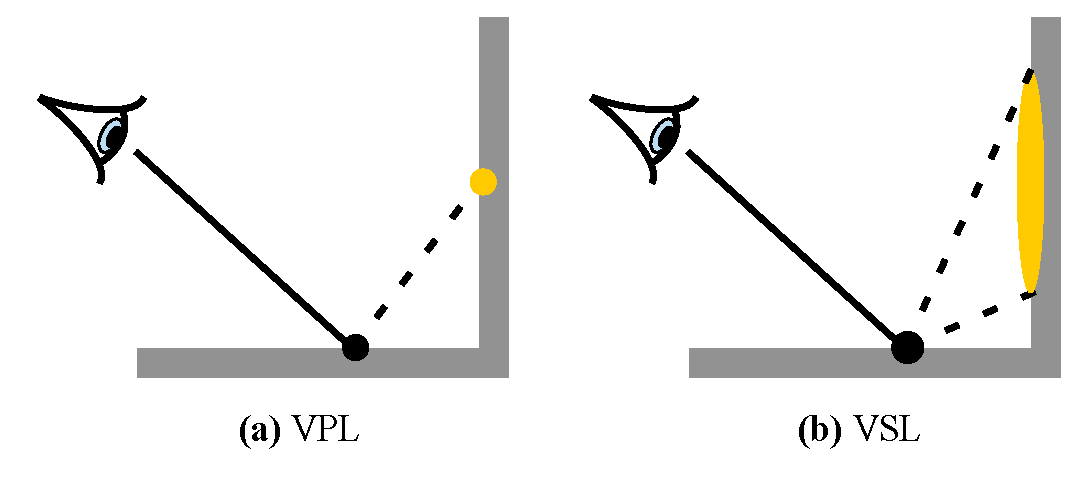
\includegraphics[width=0.65\textwidth]{figures/ir/vpl-vs-vsl}
	\caption{传统的即时辐射度方法对光照分布执行点采样(a),这容易导致奇异值;要使采样结果更加平滑,一种方式就是对采样值在使用之前执行某种形式的“过滤”,即每个值对附近核估计范围内的采样点均有贡献,这就将虚拟点光源转换为面积光源(b)}
	\label{f:ir-vpl-vs-vsl}
\end{figure}

上面的描述非常晦涩,我们需要一种更直观的解释。对虚拟点光源的过滤和光子映射中对光子的密度估计有些类似,所以\cite{a:VirtualSphericalLightsforMany-LightRenderingofGlossyScenes}甚至直接称虚拟点光源为光子光源(photon light)\myindex{光子光源}{photon light},如图\ref{f:ir-reverse-pm}所示,传统的光子映射是基于点收集的,即对每个估计顶点(黑色圆点)使用一个估计半径,然后对该球体覆盖的光子(红色圆点)进行密度估计,这个估计范围也可以反过来作用于光子上,然后每个光子可以对其估计范围内的估计点进行“溅射”,这即是\cite{a:FastFinalGatheringviaReversePhotonMapping}提出的反向光子映射,它是渐进式光子映射的基础。

\begin{figure}
	\sidecaption
	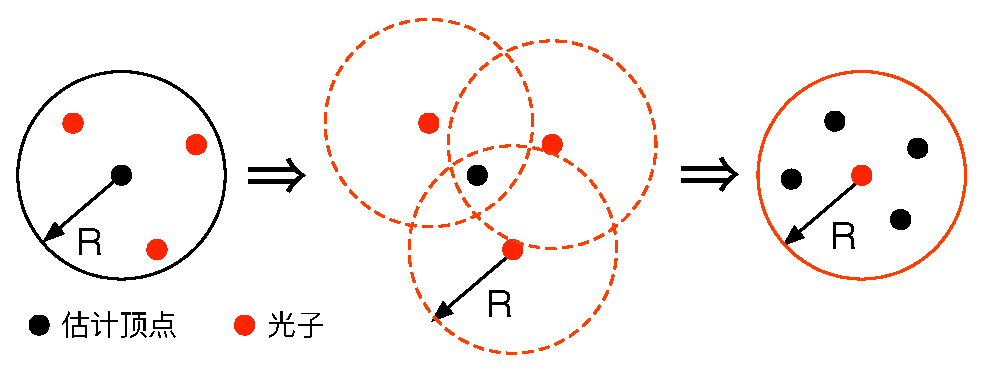
\includegraphics[width=0.65\textwidth]{figures/ir/reverse-pm}
	\caption{左图表示传统基于点收集的光子映射,每个估计顶点被使用一个过滤范围以寻找其覆盖的光子;这个估计范围可以反过来被作用于光子上,然后通过寻找其覆盖的估计顶点进行估计,这形成右图所示的反向光子映射}
	\label{f:ir-reverse-pm}
\end{figure}

光子映射中的光子都是位于漫反射表面上,因此它们的光照贡献与方向无关,所以其核估计函数仅仅是一个2D的表示位置的函数,但是这里讨论的光子光源可能位于光泽表面上,因此其光照包含有方向分布信息,因此需要一个4D的核估计函数。以下我们根据上述描述的光照传输过程推导出这个核估计函数。

与反向光子映射类似,我们可以认为每个位于位置$\mathbf{p}_j$处的光子光源对半径$r_j$内的空间均有光照贡献,这些位置$\mathbf{y}$处沿方向$\omega$的出射辐射亮度为:

\begin{equation}\label{e:ir-vpl-splatting}
	L^{splat}_j(\mathbf{y},\omega)= \cfrac{\Phi_j}{\pi r^{2}_j}f_r(\mathbf{y},\mathbf{i}_j,\omega)(||\mathbf{y}-\mathbf{p}_j||<r_j)
\end{equation}

\noindent 这里$L^{splat}_j(\mathbf{y},\omega)$即表示位于$\mathbf{p}_j$处的光子光源在以以$r_j$为半径的球体内向外溅射的辐射亮度,$\Phi_j$表示该光子光源来自$\mathbf{i}_j$方向的的辐射通量,$\pi r^{2}_j$表示对球内表面面积的一个近似,以$r_j$为半径的球体内的位置$\mathbf{y}$可以表述为$(||\mathbf{y}-\mathbf{p}_j||<r_j)$,它的值为1(点$\mathbf{y}$位于球体内)或者0(点$\mathbf{y}$位于球体外)。

\begin{figure}
	\sidecaption
	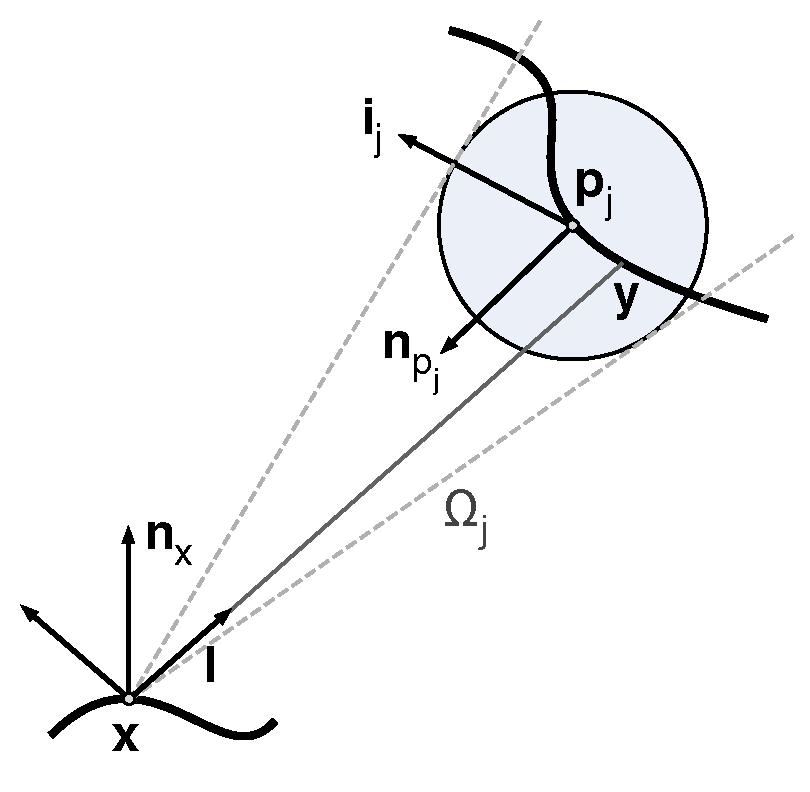
\includegraphics[width=0.37\textwidth]{figures/ir/vsl}
	\caption{虚拟球体光源,从方向$\mathbf{v}$观察表面上的顶点$\mathbf{x}$,其接受来自位于$\mathbf{p}_j$处入射方向为$\mathbf{i}_j$的虚拟球体光源的光照,该光照的值为两个顶点的BRDF分布函数以及顶点夹角的余弦的内积沿立体角$\omega_j$上的积分}
	\label{f:ir-vsl}
\end{figure}

以上我们表述出了光子光源的溅射光照分布,注意,此时还没有执行任何模糊的过程。为了计算光子光源对一个着色点的光照贡献,我们将上述的“面积光源”代入着色点的辐射亮度函数中,即:

\begin{equation}\label{e:ir-shading-point-radiance}
	L^{p}_j(\mathbf{x},\mathbf{v})={\rm \int}_{H^{2}}f_r(\mathbf{x},\mathbf{l},\mathbf{v})\cos(\mathbf{n}_x,\mathbf{l})L^{splat}_j(\mathbf{y},-\mathbf{l}){\rm d}\mathbf{l}
\end{equation}

\noindent 这里$L^{p}_j(\mathbf{x},\mathbf{v})$表示沿$\mathbf{v}$方向观察,着色顶点$\mathbf{x}$来自$\mathbf{p}$处的光子光源的光照,如图\ref{f:ir-vsl}所示,这里$H^{2}$表示着色点$\mathbf{x}$的半球面方向。

将式\ref{e:ir-vpl-splatting}代入式\ref{e:ir-shading-point-radiance}就可以得到光子光源的完整定义:

\begin{equation}\label{e:ir-photon-light}
	L^{p}_j(\mathbf{x},\mathbf{v})= \cfrac{\Phi_j}{\pi r^{2}_j}{\rm \int}_{\Omega_j}f_r(\mathbf{x},\mathbf{l},\mathbf{v})\cos(\mathbf{n}_x,\mathbf{l})f_r(\mathbf{y},\mathbf{i}_j,-\mathbf{l})(||\mathbf{y}-\mathbf{p}_j||<r_j){\rm d}\mathbf{l}
\end{equation}

\noindent 这里$\Omega_j$取代了$H^{2}$,它表示沿$\mathbf{x}$向以$\mathbf{p}_j$为球心,半径为$r_j$的球体方向的圆锥体空间,如图\ref{f:ir-vsl}所示,因为光子光源对于该圆锥体之外的空间其贡献值为0。这里函数$(||\mathbf{y}-\mathbf{p}_j||<r_j)$仍被保留的被积函数中,因为$\Omega_j$空间中的方向仍然可能穿过光子光源的球体区域。

式\ref{e:ir-photon-light}涉及在$\Omega_j$区域内的方向采样,这需要使用光线投射,其代价非常高,\cite{a:VirtualSphericalLightsforMany-LightRenderingofGlossyScenes}将式\ref{e:ir-photon-light}转换成了下述下式:

\begin{equation}\label{e:ir-vsl}
	L^{s}_j(\mathbf{x},\mathbf{v})= \cfrac{\Phi_j}{\pi r^{2}_j}V(\mathbf{x},\mathbf{p}_j){\rm \int}_{\Omega_j}f_r(\mathbf{x},\mathbf{l},\mathbf{v})\cos(\mathbf{n}_x,\mathbf{l})f_r(\mathbf{y},\mathbf{i}_j,-\mathbf{l})\cos(\mathbf{n_{\mathbf{p}_j}},-\mathbf{l}){\rm d}\mathbf{l}
\end{equation}

\noindent 该式的定义基于以下近似方法:

\begin{itemize}
	\item VSL的可见性定义为光子光源位置$\mathbf{p}_j$与着色点$\mathbf{x}$之间的可见性,这使得前面介绍的基于GPU的阴影图可以被直接使用。
	\item 球体内各个表面位置处的法线和BRDF分布函数近似为常数,它们直接使用点$\mathbf{p}_j$的参数,所以式\ref{e:ir-vsl}中的所有BRDF和余弦都仅取决于$\mathbf{x}$和$\mathbf{p}_j$。
	\item 指示是否位于球体内的函数被一个余弦项$\cos(\mathbf{n}_{\mathbf{p}_j},-\mathbf{l})$代替,例如当一个$\Omega_j$内的光线穿过球体,但是其交点$\mathbf{y}$落于球体之外时,$-\mathbf{l}$与$\mathbf{n}_{\mathbf{p}_j}$的夹角趋向于大于$90^{\circ}$,因此其余弦值小于0而被舍弃。
\end{itemize}

从式\ref{e:ir-vsl}可以看出,其虚拟点光源的4D过滤函数其实就是着色点$\mathbf{x}$处的BRDF分布函数,这使得虚拟点光源在被使用之前就被模糊处理了,因此奇异值被消除,同时能够保留光照的光泽反射特性。和光子映射类似,光子光源的核估计半径$r_j$也可以通过k-NN进行计算。

为了计算VSL的光照贡献,式\ref{e:ir-vsl}包含对$\Omega_j$方向空间的积分,这可以使用蒙特卡洛方法进行估计,为了减少估计的方差,\cite{a:VirtualSphericalLightsforMany-LightRenderingofGlossyScenes}对圆锥体空间$\Omega_j$,着色点$\mathbf{x}$和光子光源$\mathbf{p}_j$各自的BRDF分布函数进行重要性采样以提升估计质量,如图\ref{f:ir-vsl-sampling}所示。

\begin{figure}
	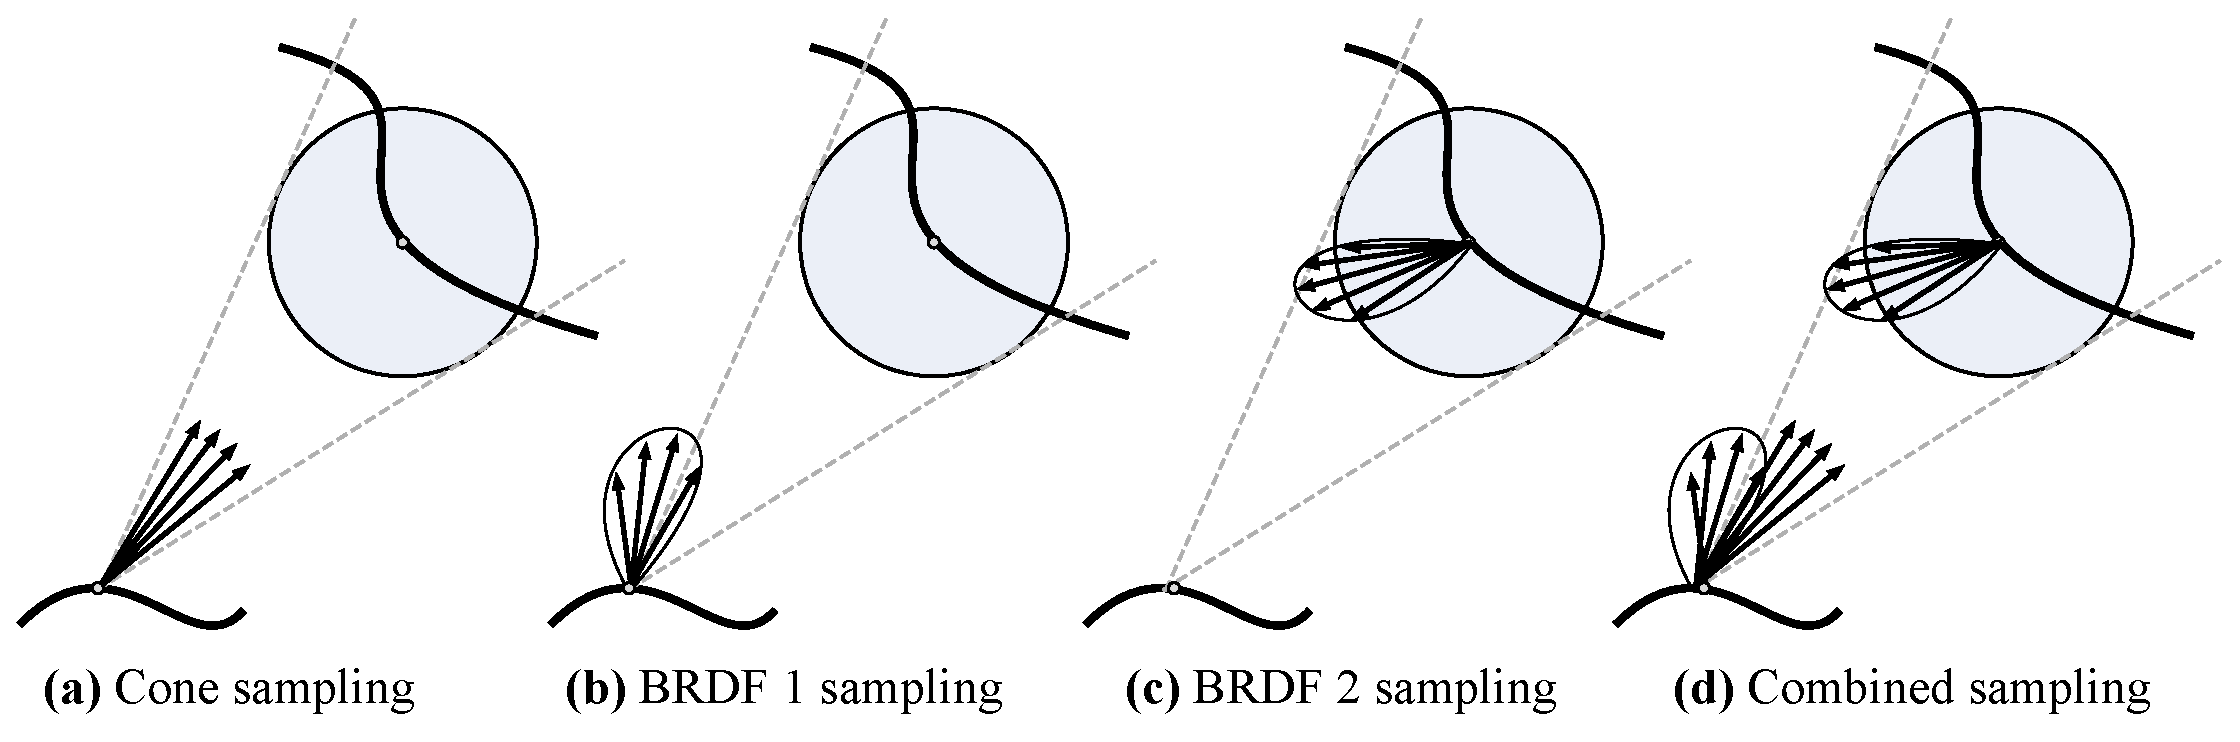
\includegraphics[width=1.0\textwidth]{figures/ir/vsl-sampling}
	\caption{对VSL的光照贡献执行重要性采样,其中(a)表示着色点向球体方向的圆锥体空间,(b)和(c)分别表示着色点和光子光源的BRDF分布函数,(b)为联合重要性采样结果,需要注意的是,(b)和(c)必须同时包含在(a)中才能对着色点形成光照贡献}
	\label{f:ir-vsl-sampling}
\end{figure}

和光子映射一样,由于模糊处理,虚拟球体光源技术引入了偏差,这些偏差可以通过增加VSL的数量来减少,同样,由于采样溅射的方法,我们可以使用类似渐进式光子映射的方式通过逐渐增加VSL的数量来提升估计的质量以及减少偏差。




\subsection{参与介质中的方法}
采样不足是即时辐射度方法中产生奇异值斑点的直接原因,由于光子光束技术(photon beams approach)\cite{a:AComprehensiveTheoryofVolumetricRadianceEstimationusingPhotonPointsandBeams,a:ProgressivePhotonBeams}的创新性工作,在参与介质中,我们可以通过存储整个路径片段而不仅仅是单个路径顶点,来大大提高光子的密度,因此也提高了估计的精度,随后这种基于光束的思路而被运用于即时辐射度方法中,它们大大增加了虚拟点光源的密度,从而减轻了奇异值斑点现象。

本节将讨论参与介质中基于光线(而不是顶点)的即时辐射度方法,这称之为虚拟光线光源技术(第\ref{sec:ir-vrl}节)。需要注意的是,和前面介绍的虚拟球体方法对样本进行模糊来避免奇异值斑点不同的是,虚拟光线光源技术仅仅是(间接)增加了虚拟点光源的密度,因此它只是减轻(而不是消除)了光斑的现象。随后介绍的虚拟光束光源技术(第\ref{sec:ir-vbl}节)则将虚拟球体光源技术的模糊思想引入到虚拟光线光源技术中,才实现了斑点的彻底消除。





\subsubsection{虚拟光线光源}\label{sec:ir-vrl}
在参与介质中,由于散射无处不在,所以我们可以将一条路径线段看做一个连续分布的虚拟点光源,而不仅仅是根据单个路径顶点创建一些离散的虚拟点光源,如图\ref{f:ir-vpl-vs-vrl}所示,基于此,\cite{a:VirtualRayLightsforRenderingSceneswithParticipatingMedia}提出了虚拟光线光源技术,路径的每个线段被当做一个虚拟光线光源(virtual ray light,VRL)\myindex{虚拟光线光源}{virtual ray light},于是基于点到点的光照值计算变成一个围绕光线光源长度上的积分,这大大增加了虚拟点光源的密度,降低了奇异值分布的严重程度,使得限定导致的偏差大大减少,有时甚至可以忽略对这部分偏差的补偿。

\begin{figure}
\begin{fullwidth}
	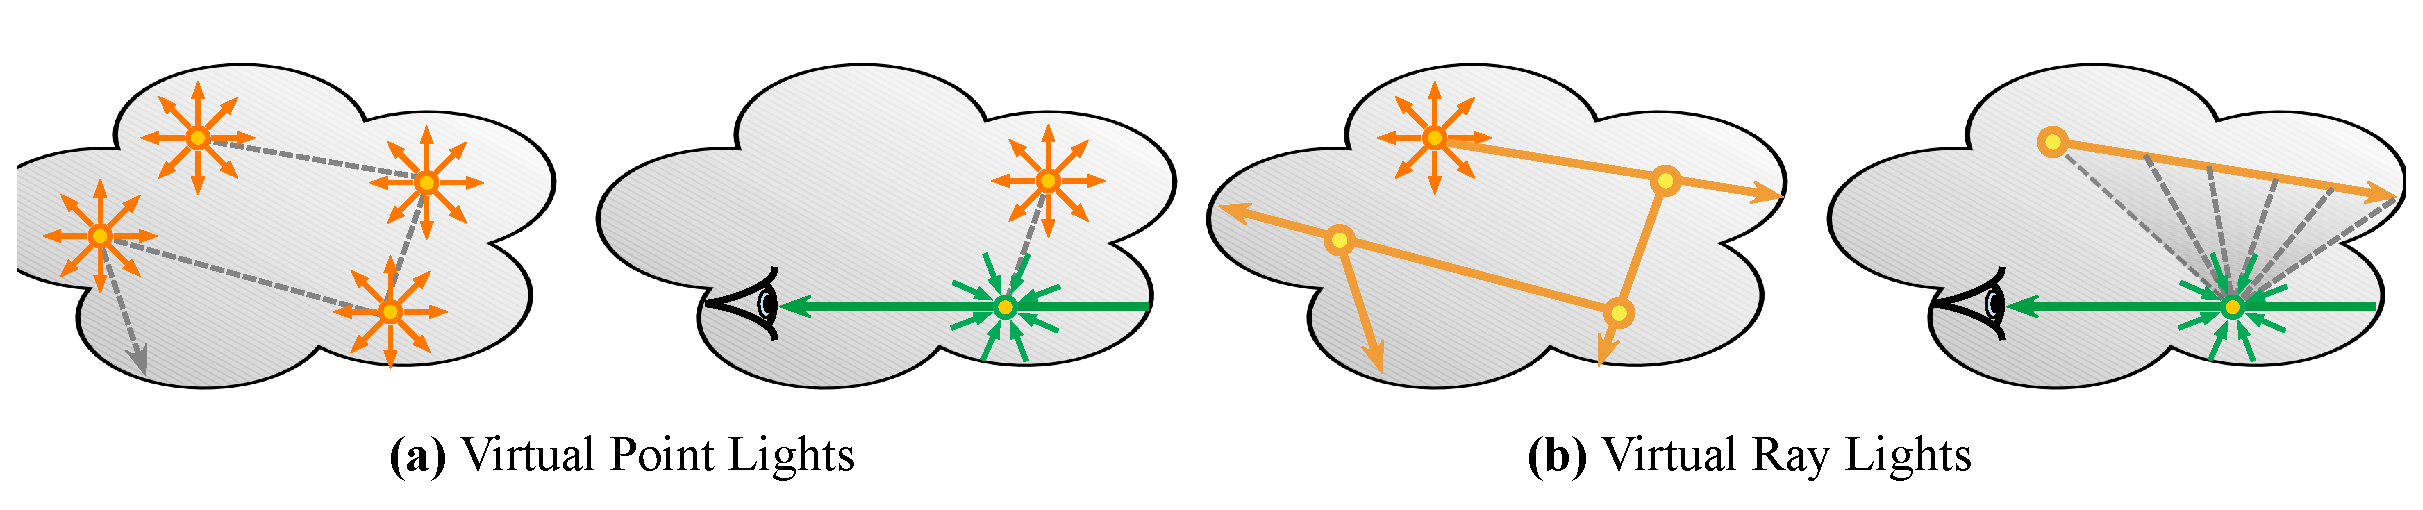
\includegraphics[width=1.\thewidth]{figures/ir/vpl-vs-vrl}
	\caption{传统的依赖于路径顶点的虚拟点光源技术(a)由于采样不足任意导致奇异值斑点,这种现象在参与介质中尤其严重;由于参与介质中的散射无处不在,所以我们可以将一条路径线段看做一个连续分布的虚拟点光源,这样每个着色点接受来自整个路径线段上的光照,这大大增加了虚拟点光源的密度(b)}
	\label{f:ir-vpl-vs-vrl}
\end{fullwidth}
\end{figure}

在虚拟光线光源技术中,路径的生成方式相较于传统的即时辐射度方法(或者光子映射中的光子)并无什么差别,例如首先对光源执行随机行走过程以生成一条光源子路径,如图\ref{f:ir-vpl-vs-vrl}(a)中那样;其唯一的不同是,对于路径中的每个顶点,一条以该顶点为起点的光线被创建,这条光线即是虚拟光源光源,它被用于后续对着色点的光照计算,如图\ref{f:ir-vpl-vs-vrl}(b)所示。

另一方面,参与介质中的着色点也不是单个顶点,摄像机光线上的每个顶点也都同时接受参与介质中的向内散射(in-scattering)光照,因此这里我们也将着色点视作一条摄像机光线,如图\ref{f:ir-vpl-vs-vrl}(b)所示,这样,一个光源子路径中的顶点对一个观察方向的光照转换为两条线段上的积分计算。以下我们就首先推导出这个双层积分的公式形式,然后讨论对该积分的数值计算方法。




\paragraph{虚拟光线光源的光照公式}
我们在第\ref{chp:pm}章已经介绍了光在参与介质中传输的一些基本知识,例如当光子在介质中传输时,消光系数$\sigma_t$决定了其传输一定距离的能量衰减,当光子与介质中的粒子发生交互时,其可能被吸收(吸收系数为$\sigma_a$),或者被散射(其散射系数为$\sigma_s$),散射的方向分布则由相位函数$f_s$决定,如果你对这些概念还不熟悉,请复习第\ref{chp:pm}章第\ref{sec:pm-participating-media}节的内容。

有了这些基本概念,我们可以用来解释虚拟光线光源对摄像机光线的光照传输过程。如图\ref{f:ir-vsl}所示,一条虚拟光线光源对一条摄像机光线的光照贡献,实际上是这两条光线上各个位置$v$和$u$之间光照的传输在两条光线长度上的积分,其中$v\in[0,t]$,$u\in[0,s]$。对于每个位置对$(v,u)$,它们之间的光照传输过程如下:

\begin{enumerate}
	\item 首先,虚拟点光源的光照$\Phi$被传输至位置$v$处,这阶段的过程受消光系数的影响(它其实是散射系数和吸收系数的和$\sigma_t=\sigma_a+\sigma_s$),消光系数的积分是一个透射比函数$T_r(v)$,我们在第\ref{chp:pm}章已经介绍了一些关于透射比函数计算的方法。
	\item 其次,当剩余的光照到达位置$v$时,它的一部分能量被吸收,其系数系数为$\sigma_v$;另一部分能量被散射,其散射的总能量由散射系数$\sigma_s$决定,只有那些散射至$u$方向的能量才会对$u$点形成光照贡献,其散射的方向分布由相位函数$f_s$决定。
	\item 然后,由$v$散射至$u$方向的光照经过透射比函数$T_r(w)$的作用后传输至$u$处;$u$处接收的光照仍然经历类似$v$处的过程(吸收和散射)后剩余能量被散射至摄像机方向。
	\item 最后,由$u$点发出的能量经历透射比函数$T_r(u)$作用后最终落于摄像机上。
\end{enumerate}

上述的过程可以表述为以下虚拟光线光源对摄像机光线的光照贡献,它是沿两条光线长度场的双重积分:

\begin{equation}\label{e:ir-vrl}
	L_m\approx\Phi{\rm \int}^{s}_0{\rm \int}^{t}_0  \cfrac{\sigma_s(u)\sigma_s(v)f_s(\theta_u)f_s(\theta_v)T_r(u)T_r(v)T_r(w)V}{w(u,v)^{2}}{\rm d}v{\rm d}u
\end{equation}

上式中各个参数对应的示意图如图\ref{f:ir-vrl}所示,其中$\Phi$表示虚拟光线光源对应路径起点处的辐射通量,$v$和$u$分别表示虚拟光线光源和摄像机光线上的采样位置,$\sigma_s(v)$和$\sigma_s(u)$分别表示$v$和$u$处的吸收系数,$f_s(\theta_v)$和$f_s(\theta_u)$表示$v$和$u$处的相位函数(其包含了散射系数和散射方向分布),$w$和$V$分别表示$v$和$u$之间的距离和可见性,$w(u,v)^{2}$表示由辐射通量向辐射亮度转换的距离递减。

\begin{figure}
	\sidecaption
	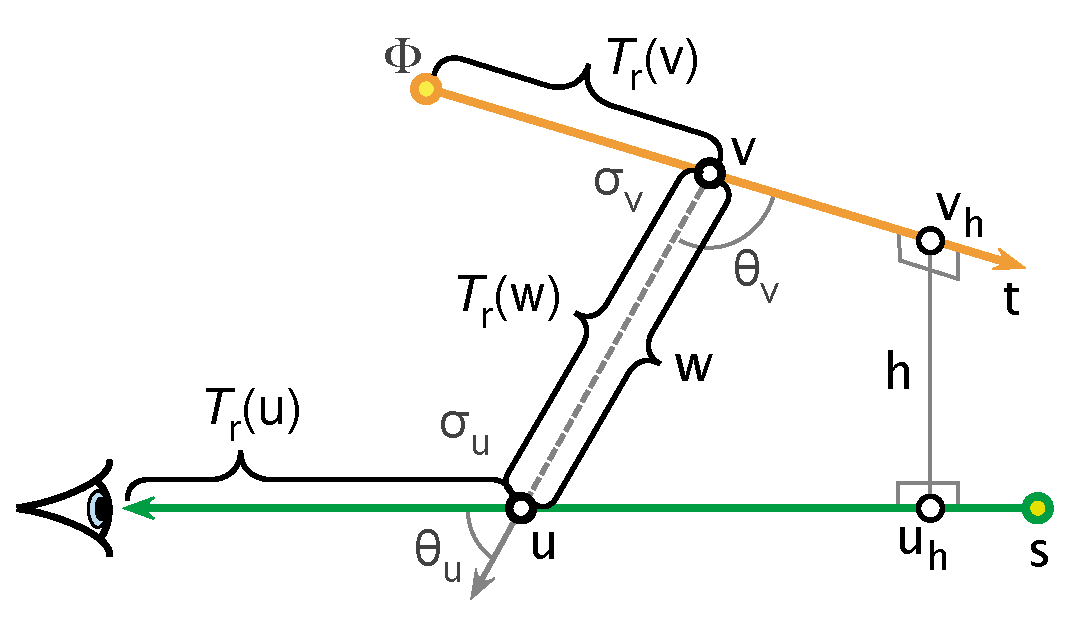
\includegraphics[width=0.6\textwidth]{figures/ir/vrl}
	\caption{虚拟光线光源(橙色)对摄像机光线(绿色)的光照贡献,其实是两条光线上每个点对($v,u$)之间贡献值的函数在两条光线长度上的积分}
	\label{f:ir-vrl}
\end{figure}

对于式\ref{e:ir-vrl},其最困难的部分来自于双重积分的计算,通常计算积分的方法是蒙特卡洛方法,这涉及对两条光线上位置的采样,但是由于式\ref{e:ir-vrl}的被积函数涉及非常多的因素,常规采样方法得到的样本方差通常比较高,为此,\cite{a:VirtualRayLightsforRenderingSceneswithParticipatingMedia}提出了一种特殊的采样方法。




\paragraph{虚拟光线光源光照传输的重要性采样}
式\ref{e:ir-vrl}定义了一个2D的积分域$(u,v)$,其中$u$表示沿摄像机光线的长度,$v$表示沿虚拟光线光源的长度。其被积函数同时包含了散射系数,相位函数,沿光源光线和摄像机光源的透射比函数,以及$v$和$u$之间的距离的平方,可见性函数,以及透射比函数,图\ref{f:ir-vrl-all}演示一个虚拟光线光源和一条摄像机光线条件下上述各个单个函数(不包含可见性)的分布,以及它们的组合分布。

一个自然的选择是对上述的各个部分的函数执行重要性采样,然后使用复合重要性采样对它们进行组合。然而通过分析图\ref{f:ir-vrl-all}可知,距离平方倒数的分布主要集中于少数区域,跟其他部分函数分布的重合度很低,此外相位函数与散射系数和透射比分布的差差异也比较大,这导致即使是使用复合重要性采样也会有很大的方差。

为此,\cite{a:VirtualRayLightsforRenderingSceneswithParticipatingMedia}提出了一个两阶段的方法,我们首先讨论各项同性散射的参与介质,以便把焦点集中于这种方法的基本思路,然后将其扩展至各项异性散射的介质。

\begin{figure}
\begin{fullwidth}
	\begin{subfigure}[b]{0.19\thewidth}
		\includegraphics[width=1.0\textwidth]{figures/ir/vrl-phase-function}
		\caption{相位函数}
	\end{subfigure}
	\begin{subfigure}[b]{0.19\thewidth}
		\includegraphics[width=1.0\textwidth]{figures/ir/vrl-scattering}
		\caption{散射系数}
	\end{subfigure}
	\begin{subfigure}[b]{0.19\thewidth}
		\includegraphics[width=1.0\textwidth]{figures/ir/vrl-transmittance}
		\caption{透射比}
	\end{subfigure}
	\begin{subfigure}[b]{0.19\thewidth}
		\includegraphics[width=1.0\textwidth]{figures/ir/vrl-inverse}
		\caption{距离平方的倒数}
	\end{subfigure}
	\begin{subfigure}[b]{0.19\thewidth}
		\includegraphics[width=1.0\textwidth]{figures/ir/vrl-all}
		\caption{组合分布}
	\end{subfigure}
	\caption{虚拟光线光源光照传输(式\ref{e:ir-vrl})被积函数各个部分的分布可视化,以及它们的组合分布,由此可以看出它们的重合度非常低,传统的复合重要性采样方法会形成比较大的方差(图片来自\cite{a:VirtualRayLightsforRenderingSceneswithParticipatingMedia})}
	\label{f:ir-vrl-all}
\end{fullwidth}
\end{figure}

在各向同性介质中,距离平方倒数的分布对积分的影响是最重要的,如图\ref{f:ir-vrl-all}(d)所示,所以我们希望得到一个正比于该项的概率密度函数,即${\rm pdf}(u_i,v_i)\propto w(u,v)^{-2}$,然而对这样的概率密度函数执行逆变换算法进行采样的计算成本比较高。

因此,这里的两阶段方法使用分析的方式得出一个联合概率分布:它首先使用一个与$u$无关的边缘概率分布函数得到样本$v_i$,然后再基于到该样本距离平方的倒数推导出一个条件概率密度函数,并对其采样得到样本$u_i$。

首先我们执行一个变量替换$\hat{u}=u-u_h$和$\hat{v}=v-v_h$,因此虚拟光线光源上变量的起点和终点可以表示为$\hat{v}_0$和$\hat{v}_1$,这里$u_h$和$v_h$表示摄像机光线距离虚拟光线光源上两个最近的位置,如图\ref{f:ir-vrl}所示,该最小距离为$h$。根据余弦定理,其距离的平方可以定义为$w(\hat{u},\hat{v},h,\theta)^{2}=h^{2}+\hat{u}^{2}+\hat{v}^{2}-2\hat{u}\hat{v}\cos\theta$,这里$\cos\theta$表示摄像机光线和虚拟光线光源之间夹角的内积。

所以,变量$\hat{v}$的边缘概率密度函数可以表述为:

\begin{equation}
	{\rm pdf}(\hat{v},\hat{v}_0,\hat{v}_1)= \cfrac{{\rm \int}^{\hat{u}_1}_{\hat{u}_0} w(\hat{u},\hat{v},h,\theta)^{-2}{\rm d}\hat{u}}{{\rm \int}^{\hat{v}_1}_{\hat{v}_0}{\rm \int}^{\hat{u}_1}_{\hat{u}_0} w(\hat{u},\hat{v},h,\theta)^{-2}{\rm d}\hat{u}{\rm d}\hat{v}}
\end{equation}

\noindent \cite{a:VirtualRayLightsforRenderingSceneswithParticipatingMedia}指出上述的积分形式在数学上并没有简单的解析方案,为此他们做了一个简化,即假设摄像机光线的长度是无限的,通过一些演算,最终可以得出两个随机变量的累积概率密度函数为:

\begin{equation}
\begin{aligned}
	{\rm cdf}^{-1}(\xi_{i,1},\hat{v}_0,\hat{v}_1)=& \cfrac{h\sinh(\text{lerp}(A(\hat{v}_0),A(\hat{v}_1),\xi_{i,1}))}{\sin\theta}\\
	{\rm cdf}^{-1}(\xi_{i,2},\hat{u}_0,\hat{u}_1)=&h\tan(\text{lerp}(B(\hat{u}_0),B(\hat{u}_1),\xi_{i,2}))
\end{aligned}	
\end{equation}

\noindent 其中,$A(x)=\sinh^{-1}( \cfrac{x}{h}\sin\theta)$,$B(x)=\tan^{-1}(x/h)$,$\xi_{i,1},\xi_{i,2}\in[0,1)$,其最终的概率密度函数为两个随机变量概率密度函数的乘积。由于该概率密度函数很好地反应了距离平方倒数的分布,因此(相对于复合重要性采样)具有较小的方差。

对于各向异性介质,其相位函数分布对采样结果的影响也非常大,例如从图\ref{f:ir-vrl-all}中可以看出其相位函数(a)和组合分布(e)具有较大的相似度,因此我们希望获得一个距离平方倒数和相位函数乘积的概率密度函数,即:

\begin{equation}
	{\rm pdf}{u_i,v_i}\propto \cfrac{f_s(\theta_u)f_s(\theta_v)}{w(u,v)^{2}}
\end{equation}

\noindent 类似于各向同性的情形,这里第一步任然是根据到一条无限长度摄像机光线距离平方的倒数关系创建样本$v_i$的边缘概率密度函数,然后以此为条件创建样本$u_i$的条件概率密度函数,最后取两者的联合。

但是各向异性的情况还是稍微复杂一点,首先对于$v_i$的边缘概率密度函数,相位函数$f_s(\theta_u)$包含的变量$u$并不任意被移除,因此很难构造边缘概率密度函数,但是观察图\ref{f:ir-vrl}可知,距离平方的倒数分布是最大的影响因素,所以第一步边缘分布的计算可以忽略相位函数的影响,直接取距离平方的倒数分布,这就变得和各向同性的情形是一致的。

\begin{figure}
	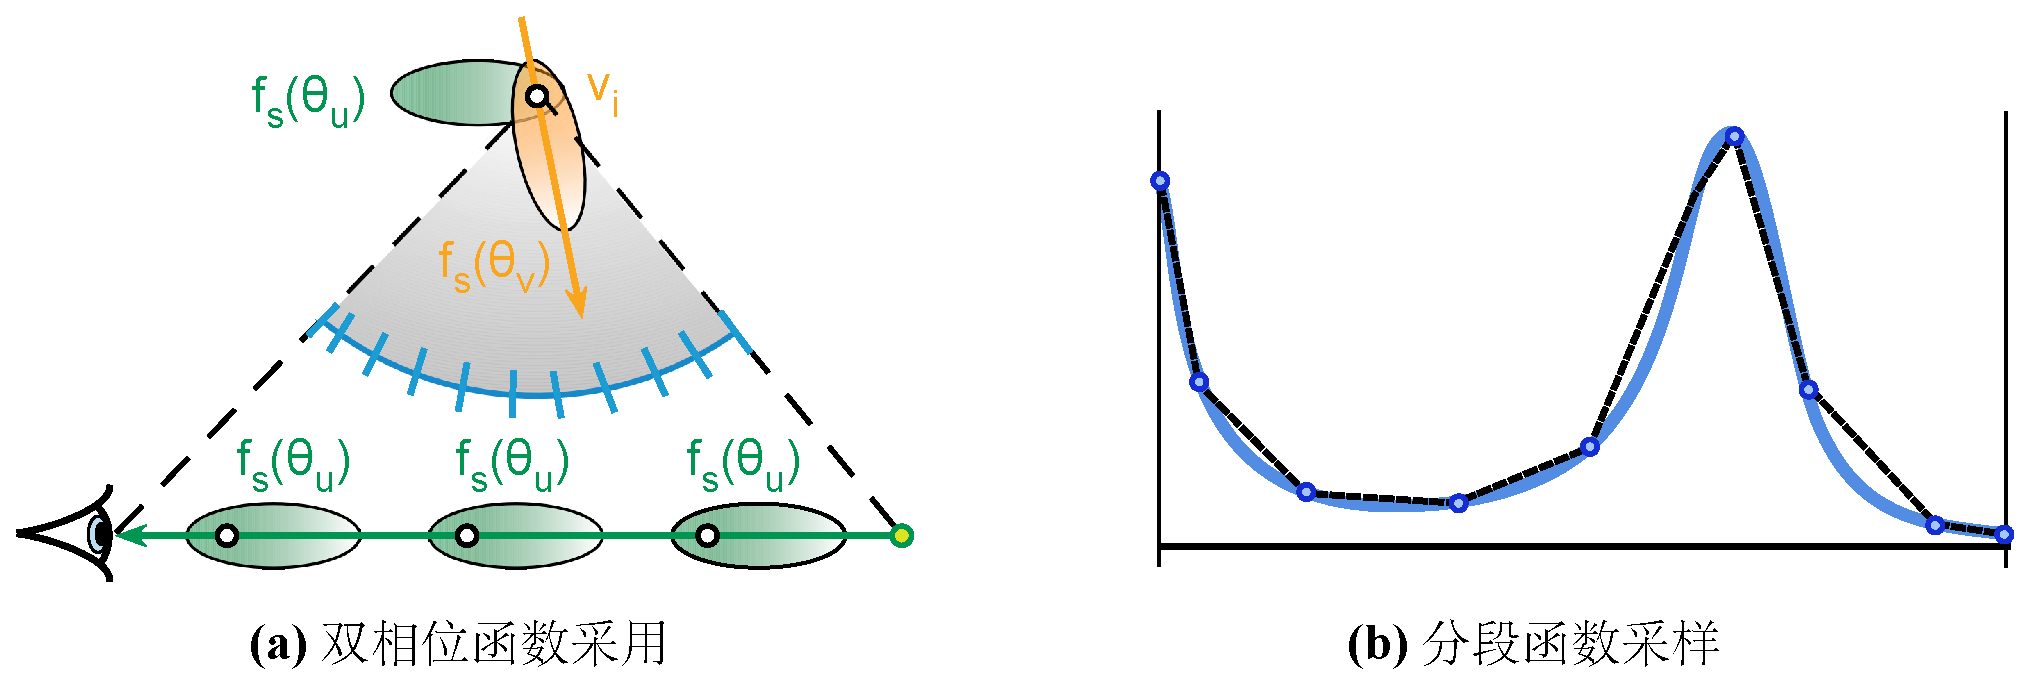
\includegraphics[width=1.\textwidth]{figures/ir/vrl-piece-wise-sampling}
	\caption{由于$v_i$已经是使用服从距离平方倒数的分布进行采样的,所以$u_i$的采样只要服从两个相位函数乘积的分布即可(a),该分布可以进一步被使用约10个点的分段线性函数进行近似(b)}
	\label{f:ir-vrl-piece-wise-sampling}
\end{figure}

对于第二项,即样本$u_i$的条件概率密度函数,由于第一项已经将分布限定于距离平方倒数分布的区域,因此距离平方倒数的影响相较于相位函数分布变得次要,所以第二项仅仅将两个相位函数的乘积作为概率密度函数,记为$f_{uv}(\theta(u_i))$,如图\ref{f:ir-vrl-piece-wise-sampling}(a)所示。\cite{a:VirtualRayLightsforRenderingSceneswithParticipatingMedia}发现使用约10个位置的分段线性函数即可以很好地近似双相位函数乘积的分布,如图\ref{f:ir-vrl-piece-wise-sampling}(b)所示,在该论文的附录部分讨论了怎样非均匀地获取这些分段顶点,并使得分段函数能够覆盖原始函数的峰值特征。




\subsubsection{虚拟光束光源}\label{sec:ir-vbl}
通过提高参与介质中虚拟点光源的密度,虚拟光线光源技术减少了即时辐射度方法的奇异值斑点现象,尽管如此,其计算过程中的奇异值仍然是存在的,因为虚拟光线技术并没有对奇异值做任何特殊处理,例如它本质上处理的还是单个虚拟点光源对单个着色点的光照(也因此虚拟光线光源技术是一种无偏估计),要想彻底消除奇异值斑点,还需要对其执行限定或者偏差补偿。

为了彻底避免奇异值,受虚拟球体光源技术的启发,\cite{a:ProgressiveVirtualBeamLights}对虚拟光线光源使用一个有限的厚度,将其扩展为虚拟光束光源(virtual beam light,VBL)\myindex{虚拟光束光源}{virtual beam light},如图\ref{f:ir-vrl-vs-vbl}(b)所示,和虚拟球体光源一样,其包含的每个虚拟点光源在使用之前被模糊处理,因此产生了更加平滑的结果。虽然模糊处理操作引入了偏差,但是同基于光束的渐进式光子映射一样,虚拟光束光源技术可以通过渐进式(减小核估计范围)的方式收敛到正确结果。

\begin{figure}
	\sidecaption
	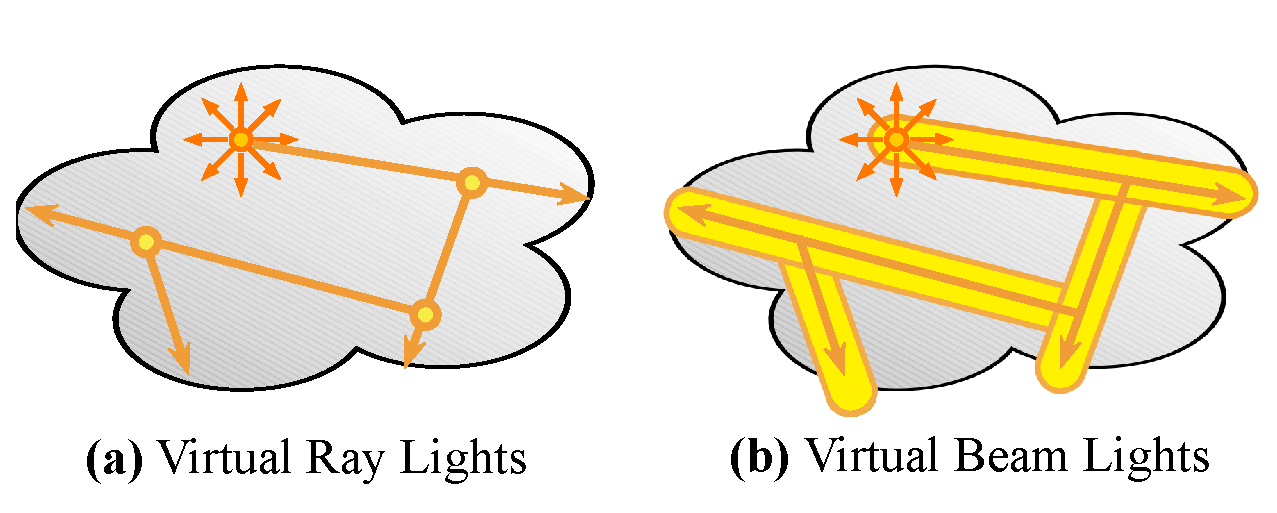
\includegraphics[width=0.65\textwidth]{figures/ir/vrl-vs-vbl}
	\caption{为了彻底消除奇异值,虚拟光束光源技术(b)将虚拟球体光源技术中的模糊处理引入至虚拟光线技术(a)中,每个虚拟点光源的光照被溅射到周围一定的模糊(球体)范围内,使形成一条光束}
	\label{f:ir-vrl-vs-vbl}
\end{figure}

相对于虚拟光线光源技术,虚拟光束光源算法的唯一区别是,式\ref{e:ir-vrl}的被积函数中的虚拟点光源(VPL)对着色点的光照,被转换为虚拟球体光源(VSL)对着色点的光照(式\ref{e:ir-vsl}),由此我们可以得到虚拟光束光源对摄像机光线的光照贡献如下:

\begin{equation}
	L_m\approx \cfrac{\Phi}{\pi R^{2}}{\rm \int}\int \sigma_s(u)T_r(u){\rm \int}_{\Omega_{\text{vsl}}}\sigma_s(v)f_s(\theta_u)f_s(\theta_v)T_r(v)T_r(w)V {\rm d}\omega {\rm d}v{\rm d}u
\end{equation}

\noindent 上式相较于式\ref{e:ir-vrl}多了一个围绕以虚拟点光源为中心,R为半径的球体内方向空间$\Omega_{\text{vsl}}$的积分,可以参见图\ref{f:ir-vsl}或者图\ref{f:ir-vbl-sampling}(a)和(b)所示,同时分母项(即距离平方的倒数)消失了,这是因为模糊处理的结果。由于$\Omega_{\text{vsl}}$内的积分要求使用光线投射计算可见性,所以这里仍然使用\cite{a:VirtualSphericalLightsforMany-LightRenderingofGlossyScenes}中提出的近似,即球体内除了相位函数之外所有的项保持为常数,因此上式可以简化为:

\begin{equation}\label{e:ir-vbl}
	L_m\approx \cfrac{\Phi}{\pi R^{2}}{\rm \int}\int \sigma_s(u)T_r(u)\sigma_s(v)T_r(v)T_r(w)V{\rm \int}_{\Omega_{\text{vsl}}}f_s(\theta_u)f_s(\theta_v) {\rm d}\omega {\rm d}v{\rm d}u
\end{equation}

\noindent 由于式\ref{e:ir-vrl}和式\ref{e:ir-vbl}主要的区别仅仅是每个虚拟点光源对每个着色点的光照贡献计算方式不同,所以这里仍然可以使用虚拟光线光源技术中的两阶段方法:即首先基于距离平方倒数的分布计算出样本$v_i$的边缘概率密度函数,然后再结合被积函数特征计算样本$u_i$的条件概率密度,例如对于虚拟光线光源技术,如果介质是各向同性的,对虚拟点光源向摄像机光线上的方向空间进行均匀采样即可;对于各向异性介质,则需要对两个相位函数的乘积进行重要性采样,如图\ref{f:ir-vrl-piece-wise-sampling}。而在虚拟光束光源技术中,由于两个相位函数的乘积还需要执行积分计算,传统的方法是对$\Omega_{\text{VSL}}$内的方向分布进行采样以对积分执行蒙特卡洛估计,这增加了计算成本,并且蒙特卡洛估计本身又增加了方差,因此\cite{a:ProgressiveVirtualBeamLights}使用了另一种近似方法。

\begin{figure}
	\sidecaption
	\includegraphics[width=.5\textwidth]{figures/ir/vbl-piece-wise-sampling}
	\caption{VRL(蓝色)和VBL(橙色)中的一个样本位置$v_i$对摄像机光线的沿角度域的光照贡献(即两个点处相位函数的乘积,即PF product)分布,从这里可以看出VBL更加平滑,并且间接地兼顾了距离平方递减。虚线线段表示对被积函数的线性分段函数表述}
	\label{f:ir-vbl-piece-wise-sampling}
\end{figure}

图\ref{f:ir-vbl-piece-wise-sampling}显式了虚拟光线光源(蓝色)和虚拟光束光源(橙色)技术中相位函数乘积的分布,由此可以看出,由于每个虚拟点光源被模糊处理,因此虚拟光束光源技术中相位函数乘积的分布要平滑得多,这意味着可以使用一个相位函数乘积的最大值函数来近似$u_i$的概率密度分布。因此,对于$u_i$的概率密度函数的每个样本(即摄像机光线上的每个顶点),我们只需要计算出样本$v_i$和$u_i$形成的方向空间$\Omega_{\text{VSL}}$内相位函数乘积的最大值即可,如图\ref{f:ir-vbl-sampling}所示,我们首先找到角度域$\Omega_{\text{VSL}}$内各个相位函数具有最大值的两个方向$\omega^{'}_{\max}$,然后分别计算这两个方向对应的相位函数乘积,最后取其最大值用来近似围绕该角度域的积分计算。

\begin{figure}
	\sidecaption
	\includegraphics[width=.65\textwidth]{figures/ir/vbl-sampling}
	\caption{为了找到角度域$\Omega_{\text{VSL}}$内相位函数乘积的最大值,首先分别寻找两个个相位函数在该作用域内的最大值,然后分别计算这两个方向$\Omega^{'}_{\max}$处的相位函数乘积,并取最大值作为积分的近似值}
	\label{f:ir-vbl-sampling}
\end{figure}

对每个虚拟顶点光源的模糊操作引入了偏差,同渐进式光子映射一样,这种偏差仍然可以通过不断减少虚拟球体光线的核估计范围来减少偏差,并使得在半径趋近于0的极限情况下,方差和偏差同时也趋近于0,这方面的知识可以参考第\ref{chp:pm}章中相关的内容。




\section{可扩展性}
在即时辐射度方法的两个基本步骤中,虚拟点光源的着色计算成本要远远高于它的生成成本\footnote{这是因为粒子的生成仅仅是与路径长度相当次数的光线投射,而每个虚拟点光源的着色计算则涉及与屏幕像素数量相当次数的光线投射,尽管这个过程可以使用阴影图来高效近似,但是每个虚拟点光源的着色计算成本仍然非常高。},并且即时辐射度方法的精确度严重依赖于虚拟点光源的数量,在传统的方法中,着色阶段的计算成本正比于虚拟点光源的数量,这使得即时辐射度方法的可扩展性受到了极大的限制,例如它很难处理一些包含大量局部细节(如光泽反射,间接阴影,近距离颜色渗透等)的场景,因为这些局部细节需要大量的虚拟点光源。

本节就来讨论在给定数量的虚拟点光源下,怎样使用近似但精确的方法是着色计算的成本与虚拟点光源的数量呈次线性(sub-linearly)\myindex{次线性}{sub-linearly}关系。我们称这些方法是可扩展(scalable)或者可伸缩的,因为这些方法计算成本增加的速度慢于虚拟点光源数量增加的速度,这使得可以使用更多(例如上百万)的虚拟点光源以获得更精确的结果。

本节将讨论的方法都基于这样的观察:即在大量的虚拟点光源中,它们的光照贡献并不是相等的,许多虚拟点光源的重要性要低于其他一些虚拟点光源,例如那些较远或者被遮挡的虚拟点光源;另一方面,少量一部分虚拟点光源可能具有非常重要的光照贡献,例如那些携带光泽反射的虚拟点光源。一种通用而具有可扩展性的方法是探索虚拟点光源的这种重要性的非均匀分布以减少计算量,这种方法对那些非常重要的虚拟点光源进行完整的计算,而对那些不重要的虚拟点光源则仅仅执行近似计算。

尽管它们各自对虚拟点光源执行重要性估计的方法不同,但是这些方法都遵循一个相同的框架,即每个方法都是将一组相似的虚拟点光源聚集成一个簇,并使得那些重要的虚拟点光源形成比较小的簇,而那些不重要的虚拟点光源形成比较大的簇。由于这些簇内的虚拟点光源都是相似的,因此它们的聚焦结果可以使用单个更亮的代理虚拟点光源(representative VPL)\myindex{代理虚拟点光源}{representative VPL}进行近似计算。如果这样的代理虚拟点光源选择并被缩放得比较合适,那么所有代理虚拟点光源近似光照的和就等效于一个分层的蒙特卡洛估计--即在每个对作用域进行分层的区间只选取一个样本近似计算。

\begin{myshaded}
	这里介绍的可扩展性方法看起来和前面介绍的适应性方法具有一定的相似性,例如都是对虚拟点光源的重要性进行估计,以减少最终着色计算的成本。这里的区别是,适应性方法聚焦于虚拟点光源的生成过程,它使得最终用于着色计算的虚拟点光源的重要性正比于它们对当前视图的光照贡献;而可扩展性方法则聚焦于着色计算阶段,它通过利用几何上近邻区域的相似性来近似计算一个簇内的虚拟点光源的光照贡献,而适应性方法对每个选择下来的虚拟点光源都执行完整(即对全部像素)的着色计算。
\end{myshaded}

本节将主要讨论三种方法,即光源切口,矩阵行--列采样,以及光源切片方法,其中光源切口方法善于处理局部光照特征,而矩阵行--列采样方法善于处理全局光照特征,光源切片方法则可以看做是上述两类方法的思路的组合。





\subsection{光源切口}
假设所有虚拟点光源的集合为$\mathds{S}$,则沿$\omega$方向观察,点$\mathbf{x}$处接收到由于所有这些虚拟点光源的辐射亮度$L$等于以下项的乘积在所有虚拟点光源上的加和,即着色点处的材质,几何项,可见性以及虚拟点光源的辐射强度:

\begin{equation}\label{e:ir-linear}
	L_{\mathds{S}}(\mathbf{x},\mathbf{\omega})=\sum_{i\in\mathds{S}}\overbrace{M_i(\mathbf{x},\mathbf{\omega})}^{\text{材质}}\underbrace{G_i(\mathbf{x})}_{\text{几何项}}\overbrace{V_i(\mathbf{x})}^{\text{可见性}}\underbrace{I_i}_{\text{辐射强度}}
\end{equation}

\noindent 由于上式是所有虚拟点光源的加和,即对所有虚拟点光源都要计算一次,所以其着色计算成本与虚拟点光源的数量成正比,为了实现可扩展性,使着色计算与虚拟点光源的数量成次线性关系,我们需要一种方法近似计算一组虚拟点光源的光照贡献,而不是像式\ref{e:ir-linear}那样分别单独完整计算每个虚拟点光源的光照。

为此,我们定义一个光源簇(light cluster)\myindex{光源簇}{light cluster},$\mathds{L}\in\mathds{S}$,它表示一组光源的集合,每个簇包含一个代理光源(representative light)\myindex{代理光源}{representative light}$j\in\mathds{L}$,然后我们将该代理光源的材质,几何项以及可见性运用于该簇内的所有虚拟点光源,则式\ref{e:ir-linear}可以变换为:

\begin{equation}\label{e:ir-sublinear}
\begin{aligned}
	L_{\mathds{L}}(\mathbf{x},\mathbf{\omega}) \approx & \sum_{i\in\mathds{L}}M_i(\mathbf{x},\mathbf{\omega})G_i(\mathbf{x})V_i(\mathbf{x})I_i\\
	= & M_j(\mathbf{x},\mathbf{\omega})G_j(\mathbf{x})V_j(\mathbf{x})\sum_{i\in\mathds{L}}I_i\\
\end{aligned}
\end{equation}

\noindent 在辐射度设置下,光源簇的辐射强度($I_{\mathds{L}}=\sum I_i$)可以被预计算并存储起来,使得整个光源簇的近似光照计算成本等于单个虚拟点光源的计算成本,只不过这里使用的是一个亮度更大的代理光源,如图\ref{f:ir-light-cluster}右边小图所示。即使在非辐射度设置条件下,由于对整个簇的光源仅执行一次(针对代理光源的)光线投射,其计算成本也大大降低。

\begin{figure}
	\sidecaption
	\includegraphics[width=0.55\textwidth]{figures/ir/light-cluster}
	\caption{光源簇表示一组相似的光源,在光源切口方法中我们使用一个更亮的(称为代理)光源来近似簇内所有光源的光照贡献}
	\label{f:ir-light-cluster}
\end{figure}

很显然,在上述方法中,每个簇的近似光照的误差取决于该簇内各个光源在材质,几何项以及可见性上的相似性(注意这里的材质项$M_i$主要指的是着色点$\mathbf{x}$处的BRDF同入射方向与法线法线夹角余弦的乘积,而$G_i$包含入射方向与光源法线夹角的余弦),这就要求我们使用一种有效的方法将相似的光源聚集成一个簇。

为了实现上述的目标,\cite{a:Lightcuts:AScalableApproachtoIllumination}提出称为光源切口的方法,该方法首先按照空间邻近性将所有虚拟点光源构造为一颗二叉树,该二叉树的非叶节点可以看做由所有子节点形成的光源簇,通过对每个着色点寻找一个合适的二叉树上节点的组合,我们就找到了一组合适的光源簇,然后通过计算式\ref{e:ir-sublinear}(而不是式\ref{e:ir-linear}),便可以大大提升着色计算的效率。




\paragraph{光源树及光源切口}
一颗光源树(light tree)\myindex{光源树}{light tree}是按照空间近邻性划分的一个二叉树,其每个叶节点是一个独立的虚拟点光源,而所有非叶节点是该其所有子节点构成的光源簇,如图\ref{f:ir-lightcuts}(a)所示。为了按照式\ref{e:ir-sublinear}对所有虚拟点光源进行空间划分,我们直接对光源树切开一个切口,一个切口(cut)是光源树中一些节点的集合,并使得对于从光源树顶点向所有叶节点形成的路径中,每个路径有且仅有一个节点位于该切口中,这个切口并形成了对所有光源的一个有效空间划分,例如在图\ref{f:ir-lightcuts}中,(b),(c)和(d)分别对应三个不同的光源切口,它们形成了对光源的不同划分。

\begin{figure}
\begin{fullwidth}
	\includegraphics[width=1.0\thewidth]{figures/ir/lightcuts}
	\caption{一个简单场景的光源二叉树(a)与几个不同的切口(b),(c)和(d),其中叶节点的数字表示光源ID,非叶结点(即光源簇)内的(灰色)数字表示簇的代理光源ID,旁边的(绿色)数字表示簇的密度(即包含光源的数量),图(b),(c)和(d)中的颜色区域表示在对应光源切口近似下与真实图像的差异比较小的区域,由此可以看出这些差异通常来自于光源附近,因为这些地方的可见性差异更大(图片来自\cite{a:Lightcuts:AScalableApproachtoIllumination})}
	\label{f:ir-lightcuts}
\end{fullwidth}
\end{figure}

虽然每一个光源切口都是对光源的一个有效划分,但是不同光源切口相对于同一着色点的计算成本和近似度是不一样的,图\ref{f:ir-lightcuts}(b),(c)和(d)中的颜色区域表示近似光照和真实光照差异较小的区域,其中图中的红色圆点所在的位置在三种不同的光源切口下具有不同的近似度,显然(c)所对应的光源切口具有更好的近似,而(b)所对应的光源切口则具有较差的近似,因此具有较大的误差。

因此,我们需要一种有效的方法能够自动根据每个着色点的位置选择合适的光源切口,然而何为“合适”,这是一个很难界定的标准。由于光源切口对光照的近似随着图像空间内像素的变化而变化,因此每个像素会使用不同的光源切口,例如其中一些像素使用一些特定级别的光源簇以减小计算成本,而另一些像素则会使用该光源簇的子节点以增加近似的精度。这种图像空间内光源切口的变化会导致令人不适的失真现象,为了阻止这种现象,我们仅仅使用那些能够保证近似误差在一定的人眼可察觉的视觉变化范围内的光源簇。这方面的依据是\cite{a:Luminancedifferencethresholds}提出的韦伯定理(Weber’s law)\myindex{韦伯定理}{Weber’s law},该定理指出人眼可察觉的最小视觉信号的变化率为1\%,因此如果我们能够保证光源切口的选择使得着色点贡献近似的误差小于1\%,那么便可以消除这种光源切口变化导致的失真。





\paragraph{光源切口的选择}
上述相对误差标准的计算要求我们能够在决定是否使用一个特定的光源簇之前对其光照贡献进行估计,这是非常困难的,因为(一些靠近叶节点位置的节点)估计的成本可能非常高。为了克服这个困难,\cite{a:Lightcuts:AScalableApproachtoIllumination}使用一种从最粗略的切口(例如光源树的根节点)开始,并渐进(递归)式的改善其精度直至满足上述误差标准的方法\footnote{这种方法和前面介绍的阶层式辐射度方法的思路其实是类似的,都是从顶点至下遍历直至满足某种终止条件,只不过这里比较的是光照值,所以使用视觉特征,而阶层式辐射度方法比较的是形状系数,所以直接使用了一个最小阈值作为终止条件。}。对于每一个节点,我们计算该光源簇的光照近似(式\ref{e:ir-sublinear}),以及该近似的一个误差上限,如果该误差上限大于指定的误差标准,则将该节点从切口中移除,并将该节点的两个子节点添加到切口中;如果该节点满足指定的误差标准,则遍历的过程结束,此时就找到了一个合适的切口,我们称这样的切口为一个光源切口(lightcut)\myindex{光源切口}{lightcut}。

光源切口方法中一个光源簇的误差是指其近似估计(式\ref{e:ir-sublinear})与真实值之间的差异,然而我们并不知道该光源簇的真实光照值,不过我们可以求出该光源簇光照贡献的最大值,这可以通过使用式\ref{e:ir-sublinear}中各项的最大值来进行计算,由于这些值都是正的,因此我们可以得出光源簇误差的最大值不会超过该光照最大值,即:

\begin{equation}
	\text{error}\leq M_{ub}G_{ub}V_{ub}\sum I_i
\end{equation}

对于可见性项,它的值为0或1,其最大值为1;对于几何项,\cite{a:Lightcuts:AScalableApproachtoIllumination}使用了一种经验方法根据光源簇的包围盒来计算其最大值,材质项的最大值也可以利用类似的方法计算而出,如图\ref{f:ir-light-cluster-error-bound}所示。计算出的光照上限与当前光源簇光照之间的差异就形成了光源簇近似的差异范围,进而被用于与指定的误差标准进行比较。

\begin{figure}
	\sidecaption
	\includegraphics[width=0.45\textwidth]{figures/ir/light-cluster-error-bound}
	\caption{每个光源簇包含一个包围盒,其被用于计算光照的最大值,这通过取该包围盒范围内各项乘数的最大值来实现}
	\label{f:ir-light-cluster-error-bound}
\end{figure}

此外,为了使处理更加高效,光源树中每个非叶子节点的代理光源被要求与其中一个子节点的代理光源相同,如图\ref{f:ir-lightcuts}所示,这使得我们在计算那个子节点时,可以重用其父节点代理光源的材质,几何及可见性项数据。

尽管光源切口方法是一种高效,可扩展的多光源方法,它仍然具有一些缺点,这些缺点主要是由于它过度估计了可见性项,即假设光源簇内的所有虚拟点光源都是可见的,这来源于上述的光照最大值计算中将可见性项设置为1,这也是光源切口方法高效的主要原因之一\footnote{这也是式\ref{e:ir-sublinear}中$V_j$可以被当做常数的原因,因为光源切口方法忽略了其他非代理光源的可见性。},因为这避免了对光源簇内所有虚拟点光源执行光线投射以计算可见性。这种对可见性的过度估计使得那些完全被遮挡的区域产生了大量额外的计算,因为很多被遮挡的区域其实际光照贡献为0。此外,光源切口方法对每个着色点都独立计算出一个光源切口,而实际上相邻像素在光源切口选择上也具有一定的相似性,后面介绍的矩阵行--列采样方法就能够利用这种特征以进一步提高计算效率。





\subsubsection{高维光源切口}
光源切口本质上是一种阶层式的方法,由于大量的处于阶层叶节点的光源具有较小的光照贡献,所以它通过从阶层自上而下的迭代,并根据一定的误差标准终止其迭代过程,以避免大量不必要的计算,从而又能够达到预期的精确度。它是一种自适应性的方法,能够自动舍弃掉那些复杂而贡献微弱的计算。基于光源切口方法,\cite{a:MultidimensionalLightcuts}提出了高维光源切口(multidimensional lightcuts)\myindex{高维光源切口}{multidimensional lightcuts}方法,该方法能够以阶层式的方式处理如参与介质,运动模糊,景深,基于空间的反走样等高维积分。

光源切口方法仅仅计算单个像素在静止场景下的光照,即针对所有虚拟点光源的积分,如式\ref{e:ir-linear}所示。对于诸如运动模糊,景深,体积光照,反走样等,\cite{a:DistributedRayTracing}指出这些效果可以表述为一个高维积分,即:

\begin{equation}\label{e:ir-multi-integrals}
	pixel={\rm \int}_{time}{\rm \int}_{volume}{\rm \int}_{aperture}{\rm \int}_{pixel area}L(x,\omega)
\end{equation}

对于上述高维积分,传统的方法(如路径追踪等)是对上述的高维作用域进行点采样,然后通过计算这些样本贡献值的加和来近似该积分计算,然而这种计算的成本非常高。受光源切口方法的启发,高维光源切口方法将阶层式的方法引入用于解决式\ref{e:ir-multi-integrals}的高维积分。

与式\ref{e:ir-linear}不同的是,式\ref{e:ir-multi-integrals}中每个像素的值是由多个像素值“混合”而来的,例如对于运动模糊,每个像素看到的是一段时间内多个着色点混合而成的模糊效果;对于反走样,它也是由一定区域内多个着色点的光照混合而成的结果;对于景深效果,它对处于焦点外的像素混合周围更大面积的像素值来形成模糊效果。因此对于式\ref{e:ir-multi-integrals},我们可以表述为对每个像素发射多个着色点光线,然后分别对每个着色点光线的光照按照某种权重进行加和以得出该像素的最终光照值。假设所有虚拟点光源的集合为$\mathds{L}$,每个像素发出的多个称为收集点(gather points)\myindex{收集点}{gather points}的集合为$\mathds{G}$,则式\ref{e:ir-multi-integrals}可以转换为多个收集点—光源对光照加和的形式:

\begin{equation}\label{e:ir-gather-light-integral}
\begin{aligned}
	pixel&=\sum_{(j,i)\in\mathds{G}\times\mathds{L}}L_{ji}\\
	     &=\sum_{(j,i)\in\mathds{G}\times\mathds{L}}S_jM_{ji}G_{ji}V_{ji}\uptau_{ji}I_i
\end{aligned}
\end{equation}

\noindent 这里$M,G,V$和$I$项与式\ref{e:ir-linear}中的意义是相同的,而$S_j$表示每个收集点的权重值,它是各种模糊效果的权重系数的乘积,其总和$\sum S_j\leq 1$。$\uptau_{ji}$表示一个二进制变量,用于限定每个收集点—光源对处于同于时刻,我们将在后面看到它的意义。

直接对式\ref{e:ir-gather-light-integral}计算所有的收集点—光源对(gather-light pair)$(g,l)$需要$\mathcal{O}(|\mathds{G}||\mathds{L}|)$的计算复杂度,高维光源切口方法通过建立一个收集点和光源的乘积图,并使用阶层式的方式对式\ref{e:ir-gather-light-integral}进行近似计算。




\paragraph{乘积图及切口}
我们的目标是要对收集点—光源对建立一个阶层式结构,就像光源切口方法中的光源树一样,然而很遗憾的是我们并不能简单地推导出这样一个阶层结构。为此,高维光源切口方法使用一个隐式方法来构造这样一个阶层结构,首先,我们分别对虚拟点光源和收集点建立一个二叉树,分别称为收集点树(gather tree)和光源树,如图\ref{f:ir-product-graph}(b)和(c)所示,这里的构造方法和前面介绍的光源切口方法中的构造方法是一样的,这些树中的每一个节点都表示该节点所有子节点(收集点或者光源)的集合,这就形成了一个隐式的关于收集点—光源对的阶层结构:$\mathds{P}=Tree(\mathds{G})\times Tree(\mathds{L})$,我们称该结构为一个乘积图(product graph)\myindex{乘积图}{product graph}。

\begin{figure}
\begin{fullwidth}
	\includegraphics[width=\thewidth]{figures/ir/product-graph}
	\caption{乘积图的构造:在式\ref{e:ir-gather-light-integral}中,每个像素光照值的计算涉及多个收集点,如(a)中的红色圆点G0和G1所示,为了得到乘积图,我们分别对收集点和虚拟点光源构建收集点树(b)和光源树(c),乘积图(c)便被表述为一个二维表格,它的每个节点是收集点树和光源树中每个节点的乘积。注意,图中的箭头表示集合构成关系,它形成一个隐式的阶层结构,蓝色节点表示叶子节点,灰色节点表示根节点}
	\label{f:ir-product-graph}
\end{fullwidth}
\end{figure}

如图\ref{f:ir-product-graph}(c)所示,乘积图并不是一棵树,而是类似于一个二维表格,它的每个节点表示收集点树中某个节点和光源树中某个节点的乘积,它的这种独特的构造方式使得我们可以隐式地得到一个收集点—光源对的阶层结构,它只需要使用两个体积更小的,阶层式的光源树和收集点树就可以得到,我们定义乘积图中每个节点表示的收集点—光源对集合为$\mathds{C}$。

接下来我们需要把切口的概念运用于上述的乘积图,由于乘积图已经隐式地建立起了所有收集点—光源对的阶层结构,我们的目标便是要适应性地选择一个“切口”并使得像素的光照近似足够精确。与光源切口方法类似,我们定义乘积图中的一个切口为乘积图中一些节点的集合,并使得对于每个叶子节点(如图\ref{f:ir-product-graph}(c)中的蓝色节点),每个由乘积图根节点(如图\ref{f:ir-product-graph}(c)中的灰色节点)向所有这些叶子节点形成的路径当中有且仅有一个节点位于切口当中,因此每个收集点—光源对仅仅可能唯一位于一个切口中的某个集合(非叶结点,或簇)当中。

有了收集点—光源对的阶层结构,与光源切口类似,我们同样使用一个代理收集点—光源对$(g,l)$来近似一个簇$\mathds{C}$的光照贡献,即有:

\begin{equation}\label{e:ir-multi-sublinear}
	\tilde{L}_{\mathds{C}}=M_{gl}G_{gl}V_{gl}\sum_{(j,i)\in\mathds{C}}S_j\uptau_{ji}I_i
\end{equation}

\noindent 上式中的材质项,几何项以及可见性项均发生于代理收集点—光源对$(g,l)$中,需要注意的是,上式右边的和式中包含$\uptau_{ji}$项,即是要求每个参与计算的收集点$g$和光源$l$必须处于同一时刻,否则估计可能会出现一些预期之外的结果,这同时也要求代理的选择满足这样的限制。

那么何为同一时刻呢?在式\ref{e:ir-multi-integrals}表示的这些效果中,每个像素的值其实是多个像素值混合的结果,然而这些参与混合的像素值并不是普通的像素值,它们是一些“不同时刻”下的“静态”像素值,例如对于运动模糊,这些混合的像素值都是不同时间下对应位置处真实的像素值,$\uptau$的限制即是要保证收集点和光源处理同一绝对时刻,这样的概念也可以推广到景深,反走样等效果,这里的时刻可以理解为一个完全静态的渲染场景,其包含特定的虚拟点光源集合以及单个收集点。

这就要求收集点树和光源树中的每个节点同时存储多个时刻下的收集点和光源,如图\ref{f:ir-multiple-representatives}所示,同时为了简化表述,我们将与时间相关的量表述为一个矢量,例如$\vec{V}$,其矢量的长度为一个固定的时刻数量$T$,矢量的每个分量表示对应时刻下的标量值,例如光源$i$存在于第二个时刻当中,其强度为$I_i=5$,假如$T=4$,则对应的矢量强度可表示为$\vec{I}_i=(0,5,0,0)$。有了上述的标记,我们便可以舍弃式\ref{e:ir-multi-sublinear}中的时间限制项$\uptau_{ji}$,形成更加简洁的表述:

\begin{equation}\label{e:ir-multi-lightcuts}
	\tilde{L}_{\mathds{C}}=M_{gl}G_{gl}V_{gl}(\vec{S}_{\mathds{C}}\cdot \vec{I}_{\mathds{C}})
\end{equation}

\noindent 在上式中,$\vec{S}_{\mathds{C}}$表示所有的收集点权重值,它可以像$\vec{I}_{\mathds{C}}$一样被缓存在收集点树的每个节点处,代理收集点—光源对$(g,l)$是满足同一时刻要求的,那么剩下的问题就是需要保证乘积图中的每个代理收集点—光源对满足同一时刻要求。




\paragraph{代理收集点—光源对的选择}
为了估计一个乘积图中一个节点的光照,根据式\ref{e:ir-multi-lightcuts},我们需要对该簇选择一个代理收集点—光源对$(g,l)\in\mathds{C}$,为了使估计无偏,其代理选择的概率为:

\begin{equation}
	p_{\mathds{C}}(g,l)= \cfrac{(\vec{S}_g \cdot \vec{I}_l)}{(\vec{S}_{\mathds{C}}\cdot \vec{I}_{\mathds{C}})}
\end{equation}

\noindent 上式中要求收集点$g$和光源是$l$是处于同一时刻的,其中$\vec{S}_g$和$\vec{I}_l$表示选定时刻$t$下代理收集点$g$的权重和代理光源$l$的辐射强度,根据上面的矢量定义可知这两个矢量仅在选定的时刻分量上具有非零值。$\vec{S}_{\mathds{C}}$和$\vec{I}_{\mathds{C}}$则分别表示该簇内所有收集点的权重加和,以及所有光源的辐射强度加和。

为了提高代理收集点—光源对查找的效率,\cite{a:MultidimensionalLightcuts}将式\ref{e:ir-multi-lightcuts}拆分成三个部分,即$p_{\mathds{C}}(g,l)=p_{\mathds{C}}(t)p_{\mathds{C}}(g|t)p_{\mathds{C}}(l|t)$,其中$p_{\mathds{C}}(t)$表示选择一个时刻$t$的概率,它等于该节点对应时刻$t$下所有子节点权重和强度的乘积站所有时刻下所有权重和强度乘积的和,即:

\begin{equation}\label{e:ir-representative-t}
	p_{\mathds{C}}(t)=( \cfrac{\vec{S}_{\mathds{C}}\cdot\hat{e}_t)( \vec{I}_{\mathds{C}}\cdot\hat{e}_t}{\vec{S}_{\mathds{C}}\cdot\vec{I}_{\mathds{C}}}
\end{equation}

\noindent $p_{\mathds{C}}(g|t)$表示$t$时刻下代理收集点$g$的权重值占所有子节点总权重值的比值:

\begin{equation}\label{e:ir-representative-g}
	p_{\mathds{C}}(g|t)= \cfrac{\vec{S}_g\cdot\hat{e}_t}{\vec{S}_{\mathds{C}}\cdot\hat{e}_t}
\end{equation}

\noindent $p_{\mathds{C}}(l|t)$表示$t$时刻下代理光源$l$的光照强度占所有子节点总光照强度的比值:

\begin{equation}\label{e:ir-representative-l}
	p_{\mathds{C}}(l|t)= \cfrac{\vec{I}_l\cdot\hat{e}_t}{\vec{I}_{\mathds{C}}\cdot\hat{e}_t}
\end{equation}

\noindent 上述的划分简化了概率计算,并且保证每个选择出来的代理收集点—光源对总是处于同一时刻;并且,由于$p_{\mathds{C}}(g|t)$仅仅依赖于收集点,所以每个时刻的代理收集点可以在建立收集点树的时候选择并缓存起来供快速查询,与之相似,$p_{\mathds{C}}(l|t)$仅仅依赖于光源,所以也可以在建立光源树的时候被计算并缓存起来。

\begin{figure}
\begin{fullwidth}
	\includegraphics[width=1.0\thewidth]{figures/ir/multiple-representatives}
	\caption{多代理点表述:为了使乘积图中的节点能够选择任意时刻下的代理收集点—光源对,我们需要对收集点树和光源树存储多个时刻下的代理点,这些代理点在构建这些树的时候选择并存储起来,然后被用于式\ref{e:ir-representative-t},\ref{e:ir-representative-g}和\ref{e:ir-representative-l}的快速计算}
	\label{f:ir-multiple-representatives}
\end{fullwidth}
\end{figure}

这就要求收集点树和光源树在建立的时候需要对每个时刻选择一个代理点(收集点或者光源),如图\ref{f:ir-multiple-representatives}所示。同时,与光源切口类似,每个父节点的某个时刻下的代理点与其中一个子节点贡献,这可以提升迭代的效率。

最后,我们简要总结一下高维光源切口方法的步骤。首先,在一个前置步骤,我们需要将时间划分为$T$个时刻,按照传统方法生成光源树,然后对每个像素,从摄像机发射多个收集点并建立收集点树,在这些树的建立过程中,还需要同时计算并存储图\ref{f:ir-multiple-representatives}所示的多代理点数据。在这之后,我们将收集点树和光源树的根节点相乘构成乘积图隐式阶层结构的根节点,它同时也是乘积图的一个最粗糙的切口,然后迭代进行一下过程:

\begin{enumerate}
	\item 选择切口中误差上限最大的节点,如果这个误差上限小于给定的误差阈值,则迭代结束。
	\item 否则我们将该节点进行进一步迭代,这通过移除该节点并使用其两个子节点进行替代来实现,由于该节点是乘积图中的节点,它是收集点树和光源树中两个节点的乘积,所以这一过程可以通过选择收集点树或光源树来实现,\cite{a:MultidimensionalLightcuts}包含了该选择的启发式。
	\item 接下来我们需要计算两个新节点的光照近似(式\ref{e:ir-multi-lightcuts}),其中一个子节点会重用父节点的代理点,而另一个子节点需要随机选择一个新的时刻以及代理点对,因此每此迭代仅仅需要执行一次计算。
	\item 最后,对上述两个新节点计算误差上限,然后返回步骤1。
\end{enumerate}

例如在图\ref{f:ir-multiple-representatives}中,切口从根节点$(G_2,L_6)$开始,其代理为时刻$t_1$下的$(G_1,L_1)$;如果递归的过程选择了$(G_2,L_4)$和$(G_2,L_5)$,即在上面的第2步中选择了对光源树节点进行递归,此时了$(G_2,L_4)$可能重用父节点的代理对$(G_1,L_1)$,而$(G_2,L_5)$,则需要需要选择一个新的时刻$t_0$下的代理对$(G_0,L_2)$,上述的过程重复进行。

由此可以看出,在上面第2步中,尽管我们仅仅根据一定的启发式选择对收集点树或光源树进行迭代,但是没有被选择的树(例如上例中的$G_2$)被保留下来,它们将在与后面子节点的比较中变得更加粗糙而进一步增大被选择的概率,通过这样的机制,乘积图实现了一个隐式的阶层结构及递归方法。




\subsection{矩阵行--列采样}
光源切口算法针对每个像素(或着色点)对光源执行一个不同的分簇,并在每个簇内选择一个代理光源以近似该簇的光照,这大大减少了对虚拟点光源执行可见性测试的数量,提升了像素着色的性能。然而光源切口算法的缺点是每个像素独立使用一个不同的光源切口,因此它不能探索相邻像素之间可能存在的相似性,并且由于需要具有对任意着色点和虚拟点光源执行可见性测试的能力,因此它只能使用计算光线投射的方法,例如不能使用现代图形处理器高效并行计算的特征。

\begin{figure}
	\sidecaption
	\includegraphics[width=0.65\textwidth]{figures/ir/matrix-interpretation}
	\caption{$m$个虚拟点光源对$n$个像素的光照构成了一个$m\times n$的传输矩阵,其中第$i$行表示第$i$个像素接收到来自所有虚拟点光源的光照(右上图),而第$j$列表示第$j$个虚拟点光源对所有像素的光照(下面三幅小图),对传输矩阵的行或列进行处理均可以利用图形处理器的并行特征(图片来自\cite{a:MatrixRow-ColumnSamplingfortheMany-LightProblem})}
	\label{f:ir-matrix-interpretation}
\end{figure}

在即时辐射度算法中,所有虚拟点光源对所有像素形成直接照射,因此我们可以构建一个传输矩阵$\mathbf{A}$,其中列为$m$个虚拟点光源,行为$n$个像素点,元素$\mathbf{A}_{ij}$表示第$j$个光源对第$i$个像素的光照贡献,矩阵$\mathbf{A}$的行表示每个像素接收来自所有光源的光照,而列表示每个光源对所有像素(整个图像)的光照,如图\ref{f:ir-matrix-interpretation}所示。定义第$j$列表示的第$j$个光源对所有像素的能量贡献为$\varphi_j$,则所有像素接收来自所有光源的光照可以表述为下述列的加和形式:

\begin{equation}\label{e:ir-column-sum-estimate}
	\mathsmaller\sum\nolimits_{\mathbf{A}}= \sum^{n}_{j=1}\varphi_j
\end{equation}

\noindent 然而直接按照上述方法对光照传输进行计算需要花费的时间复杂度为$\mathcal{O}(mn)$,这也是最原始的即时辐射度方法,我们需要一些更高效的方法来降低计算的复杂度。观察图\ref{f:ir-low-rank-matrix}所示的一个简单场景的传输矩阵示例,左上角的小图为一个$30\times 30$像素的简单场景,右边小图为其对应的传输矩阵,其列为$900=30\times 30$个像素,行为$643$个虚拟点光源。通过观察该传输矩阵,我们发现它具有比较结构化的特征,并且是低秩的,这意味着我们可以使用一个原传输矩阵的一个子集来近似其光照传输,这可以大大加速光照传输的计算。

\begin{figure}
	\sidecaption
	\includegraphics[width=0.5\textwidth]{figures/ir/low-rank-matrix}
	\caption{一个简单场景(左)及其传输矩阵(右),可以看出传输矩阵通常具有某种结构化特征,例如单个列的元素通常是相似的,这使我们可以使用一个缩减(低秩)的列矩阵来近似原始传输矩阵(图片来自\cite{a:MatrixRow-ColumnSamplingfortheMany-LightProblem})}
	\label{f:ir-low-rank-matrix}
\end{figure}

图\ref{f:ir-low-rank-matrix}到底蕴藏这什么信息呢?我们发现它的每个列中的元素几乎都是相似的,并且表现出更强的低秩特征,而行的分散则要均匀得多。我们可以推想这可能主要跟光源的强度(当然也和距离)相关,假设在忽略可见性的情况下,较强(或者较近)的光源对所有像素都有极大的贡献,而较弱(或者较远)的光源贡献则很小。

基于上述的观察,我们期望得到一个“缩减版”的传输矩阵,然后利用该缩减版的矩阵的线性组合来近似原始矩阵的光照传输,它能捕捉原始传输矩阵的重要特征,同时减少了像素着色的计算量,这正是\cite{a:MatrixRow-ColumnSamplingfortheMany-LightProblem}提出的矩阵行-列采样(matrix row-column sampling)\myindex{矩阵行-列采样}{matrix row-column sampling}算法的核心思想。从算法上看,矩阵行-列采样借鉴了光源切口的思想,它首先对传输矩阵的列进行分簇(clustering),然后对每个簇选择一个代理列(光源),最后用这些代理列来近似整个图像的颜色。然而与光源切口方法不同的是,这里光源的分簇是针对整个图像(而不是单个像素)的,因此它的光源分簇操作只需要执行一次(而不是像光源切口对所有像素都独立执行一次),然后重用于所有像素,并且由于每次针对整个列(或行)进行计算,它可以充分利用GPU的并行计算优势,使其效能数倍于光源切口方法。

与光源切口方法不同的是,矩阵行-列采样并没有像光源切口方法一样使用一种阶层式的迭代结构,而是通过对传输矩阵的行和列进行采样来得到对列的分簇,这些行列采样方法也是矩阵行-列采样方法的重点。




\paragraph{最小误差标准}
让我们再梳理一下本节关于可扩展性方法的基本思路,它们都涉及两个基本过程,即分簇(clustering)和代理选择(representative selection),其中分簇的目标是要使得最终估计的误差最小化或者尽可能地小(于某个阈值),而簇内代理的选择要使整个估计保持无偏。拿光源切口来进行分析,首先它并没有一个明确直接的分簇算法,而是简单地将光源按照空间相邻性和方向分布构建一个阶层结构,然后使用迭代地方式从上自下查找满足误差条件的簇划分,即一个光源切口;对于代理光源的选择,它是按照簇内光源的光照强度分布进行采样选取。

如果说光源切口是一种间接(或者说适应性)的分簇算法,那么这里讨论的矩阵行-列采样方法则是一种直接分簇算法,它直接根据某种误差最小化标准对光源按照对整个图像光照贡献(即传输矩阵的列)进行分簇,然后将分簇后的结果(包括代理选择)用于最终全部像素的光照计算。这里我们首先介绍其分簇的误差标准,然后在讨论具体的分簇算法。

为了对估计误差进行分析,我们需要首先得到一个使用分簇后的列进行近似的估计形式。假设已经得到对矩阵列的一个分簇结果,其将$n$个列划分成$c$个簇,由于在每个簇中只选择一个代理列进行估计,所以参与估计的矩阵实际上只是$c$个列,我们称这些列为缩减列(reduced column)\myindex{缩减列}{reduced column},其每个列记为$\rho_j$,它可以看成是对原始矩阵列$\varphi_j$向下采样(down sampling)的结果,这些缩减列形成的矩阵记为$\mathbf{R}$。由于$\varphi_j$或者$\rho_j$均表示一个列矢量,为了对列的贡献值进行比较,我们定义范数$||\rho_j||$为光源$j$对图像光照贡献的测度,并定义整个簇$C_i$内光源对图像的光照贡献测度为$s_i=\sum_{j\in C_i}||\rho_j||$。

有了上述这些术语定义,我们的目标是要对缩减矩阵$\mathbf{R}$定义一个蒙特卡洛估计$X_{\mathbf{R}}$,并使得其期望$E[X_{\mathbf{R}}]=\sum_{\mathbf{A}}$,即式\ref{e:ir-column-sum-estimate}。由于缩减矩阵$\mathbf{R}$包含$c$个列,因此其估计可以定义为这$c$个列估计的加和,即$X_{\mathbf{R}}=\sum^{c}_{i=1}X^{i}_{\mathbf{R}}$,其中$X^{i}_{\mathbf{R}}$表示对簇$C_i$的估计,因为它仅仅是选择簇$C_i$内的一个代理光源作为估计值,所以可以定义为:

\begin{equation}
	X^{i}_{\mathbf{R}}= \cfrac{s_i}{||\rho_j||}\varphi_j \text{, 其概率为 }  \cfrac{||\rho_j||}{s_i}
\end{equation}

\noindent 换句话说,我们在每个簇内选择一个代理光源对该簇进行估计(近似),其中每个代理光源没选择的概率正比于该代理光源的光照贡献测试($||\rho_j||$)与整个簇内光照贡献($s_i$)的比值。

假设$||\rho_j||>0$,则可以很容易证明上述估计是无偏的,即:

\begin{equation}\label{e:ir-reduced-estimator}
	E[X_{\mathbf{R}}]=\sum^{c}_{i=1}E[X^{i}_{\mathbf{R}}]=\sum^{c}_{i=1}\sum_{j\in C_i} \cfrac{||\rho_j||}{s_i} \cfrac{s_i}{||\rho_j||}\rho_j=\sum^{c}_{i=1}\sum_{j\in C_i}\rho_j=\sum^{n}_{j=1}\rho_j
\end{equation}

\noindent 很显然上述的估计和式\ref{e:ir-column-sum-estimate}是相同的,只不过式\ref{e:ir-reduced-estimator}会使用少得多的样本。

有了上述的基于簇的估计形式,接下来我们需要寻找让该估计误差最小化的方法来指导后面介绍的分簇算法,即我们需要寻找能够最小化$E[||X_{\mathbf{R}}-\sum_{\mathbf{R}}||^{2}]$的分簇算法,\cite{a:MatrixRow-ColumnSamplingfortheMany-LightProblem}指出该误差的期望可以表述为:

\begin{equation}\label{e:ir-reduced-estimator-error}
	E[||X_{\mathbf{R}}-\mathsmaller\sum\nolimits_ {\mathbf{R}}||^{2}]= \cfrac{1}{2}\sum^{c}_{k=1}\sum_{i,j\in C_k}||\rho_i||\cdot ||\rho_j||\cdot||\bar{\rho}_i-\bar{\rho}_j||^{2}
\end{equation}

\noindent 这里$\bar{x}$为归一化的$x$,即$x/||x||$。我们定义矢量$x$和$y$之间的“距离”为$d(x,y)= \cfrac{1}{2}||x||\cdot||y||\cdot||\bar{x}-\bar{y}||^{2}$,将原始矩阵$\mathbf{A}$的所有列矢量表示成一个$n$个顶点的图,其中每两个顶点$i$和$j$之间的连接成本为$d(\rho_i,\rho_j)$,则我们可以将误差最小化的问题转换为:将整个图划分成$c$个部分,并使每个部分内顶点之间的连接成本是最小的。

影响距离$d$的其中一个因素是同一簇内两个光源对图像光照贡献的差异,因为$||\bar{\rho}_i-\bar{\rho}_j||^{2}$是两个列矢量差的平方,即是每个分量(针对每个像素光照贡献)差的平方的和,例如虽然两个光源对图像的总能量贡献差不多,但假如它们对单个像素的光照贡献差异比较大,这也将导致两者之间的距离比较大;另一方面,两个光源各自的光照贡献$||x||$和$||y||$也影响着距离的大小,我们接下来将用式\ref{e:ir-reduced-estimator-error}的特征推导出一个高效的分簇算法。




\paragraph{分簇算法}
上述的目标函数(式\ref{e:ir-reduced-estimator-error})类似于加权K-平均值问题(weighted $k$-cluster problem)\myindex{加权K-平均值问题}{weighted $k$-cluster problem},它输入由点集$x_1,\cdots,x_n$构成的图,每个顶点的权重为$w_1,\cdots,w_n$,其目标是要将这些点划分成$k$个簇,使得下式最小化:

\begin{equation}\label{e:ir-k-cluster-problem}
	\sum^{k}_{p=1}\sum_{i,j\in C_p}w_i\cdot w_j\cdot||x_i-x_j||^{2}
\end{equation}

\noindent 这里的矩阵列分簇算法是该问题的一个特殊情况,其中$k:=c,x_i:=\bar{\rho}_i$,以及$w_i:=||\rho_i||$。为了对应上述的问题,我们将缩减矩阵转换为一个图,其包括每个列的“权重”以及“位置”,如图\ref{f:ir-reduced-columns}(a)和(b)所示,其中图中每个顶点的半径(或面积)正比于对应列的范数$||\rho_j||$,其位置分布对应于这些列的归一化矢量(如$\bar{\rho}_j$),例如在图\ref{f:ir-reduced-columns}中,相互靠近的圆意味着彼此的光源贡献比较相似。

\begin{figure}
\begin{fullwidth}
	\includegraphics[width=1.0\thewidth]{figures/ir/reduced-columns}
	\caption{缩减矩阵的列(a)可以被虚拟化为一个由圆构成的图(b),其圆的半径表示列的范数,而圆之间的位置表示列之间光照贡献的差异;(c)展示了一个符合误差最小化要求的分簇}
	\label{f:ir-reduced-columns}
\end{fullwidth}
\end{figure}

针对式\ref{e:ir-reduced-estimator-error}的要求,图\ref{f:ir-reduced-columns}(c)展示了一个列分簇的示例,例如光照贡献较小的圆往往相对没有那么重要,因为式\ref{e:ir-reduced-estimator-error}中$||\rho_i||\cdot||\rho_j||$项比较小,所以更多的光源可以被聚集到一起;光照贡献较强的光源虽然$||\rho_i||\cdot||\rho_j||$项比较大,但是如果彼此非常靠近(相似),即$||\bar{\rho}_i-\bar{\rho}_j||^{2}$项很小,则它们聚集在一起也能够产生较小的误差;此外,在相互靠近的情况下,不同强度的光源也可以聚集在一起。

针对按照将式\ref{e:ir-k-cluster-problem}最小化进行分簇问题,在已知图中所有点集信息(如权重和位置矢量)的情况下,\cite{a:ClusteredDeferredandForwardShading}提出了一种采样方法,该方法首先从给定点集中随机选择$c$个顶点作为$c$个簇的中心位置,我们可以称之为种子顶点,然后将剩下的顶点分配到距离最近的簇当中。\cite{a:MatrixRow-ColumnSamplingfortheMany-LightProblem}对其进行了修改,这里首先定义$a_i$为图上第$i$个顶点与其他所有顶点的连接成本,即:

\begin{equation}
	a_i=\sum^{n}_{j=1}d(\rho_i,\rho_j)
\end{equation}

\noindent 有了上述定义之后,我们让每个种子顶点$i$被选择的概率$p_i$正比于$a_i$,直观上看,这使得相互距离更远的顶点更容易被选择,从而保证每个簇之间的差异更大,而相似顶点更容易(在第二个步骤中)被划分到附近的簇中,而不是形成独立的簇。在实际操作中,为了产生$c$个簇,我们设置一个长度为$c$的集合,其中每个元素包含权重信息,当第$i$个顶点被选择时,我们将其添加到集合中并设置其权重为$1/p_i$,如果一个元素已经存在于集合中,则将其权重增加$1/p_i$,上述过程迭代执行直到集合中包含$c$个元素。最终,上述这些选择出来的顶点被当做$c$个簇的中心点,并且它们的权重被按照集合中的权重值缩放,然后遍历其他顶点,将其添加到与其连接成本(即$d$)最低的簇当中。

这就面临一个重要问题,在传输矩阵$\mathbf{A}$未知的情况下,怎样计算每个列(光源)的光照$\rho_i$,因为这正是我们需要求解的问题。为了解决这个问题,\cite{a:MatrixRow-ColumnSamplingfortheMany-LightProblem}对原书传输矩阵的行进行下采样,即本质上是用一个低分辨率的图像来近似光源的光照贡献计算,这可以直接通过将光源放置于摄像机处,渲染一个低分辨率的阴影图来实现。这一步称为行采样(row sampling)\myindex{行采样}{row sampling},它可以使用简单的均匀或分层采样,这是因为传输矩阵的行分布通常是均匀的,如图\ref{f:ir-low-rank-matrix}所示。所以这一个行—列采样的组合就称为矩阵行-列采样(matrix row-column sampling)\myindex{矩阵行-列采样}{matrix row-column sampling}方法。

尽管上述的采样方法非常高效,但是由于随机事件的原因,并且簇的数量$c$非常低,所以它容易产生采样不足或者过度采样的情况。对于这种随机采样的问题,往往需要确定性的方法才能解决,一种比较简单的方法就是直接对顶点(按照成本$d$)进行空间划分,例如类似于k-d树,但需要注意的是,这里的顶点之间没有实际意义上的位置和距离,我们仅能通过顶点之间的连接成本来进行度量。为了对顶点进行划分,我们可以首先将所有顶点当做一个大簇,然后对其进行分割直到达到$c$个簇。这里分离的算法很重要,\cite{a:MatrixRow-ColumnSamplingfortheMany-LightProblem}提供一种简单的方法:首先将簇$C$内的所有顶点投影到一个随机的直线上(注意每个顶点,即传输矩阵的一个列,是一个$r\times 1$的矢量,这里$r$为上面行采样的结果数量),然后在直线上找到一个最好的位置将该直线划分为两端。

\begin{figure}
	\sidecaption
	\includegraphics[width=0.55\textwidth]{figures/ir/combine-clustering}
	\caption{为了得到$c$个簇,可以先按照采样方法得到部分(如$ \cfrac{2}{3}c$)簇的划分,然后对这些簇执行分割算法知道满足$c$个簇的数量要求,这里黑色线段表示分割算法中的分割线段,其中三个比较大的簇被分割为更小的簇}
	\label{f:ir-combine-clustering}
\end{figure}

尽管直接分割方法不容易产生随机方法的问题,但是计算成本非常高,\cite{a:MatrixRow-ColumnSamplingfortheMany-LightProblem}最终使用了上述两种方法的一种组合,如图\ref{f:ir-combine-clustering}所示,对于一个给定传输矩阵的列组成的图,它首先使用采样方法生成$ \cfrac{2}{3}c$个簇,然后对这些簇执行分割,直到达到$c$个簇。将分割方法限定在一些相对较小的簇中,降低了分割算法的计算成本。

最后总结一下矩阵行-列采样方法的基本过程,如图\ref{f:ir-matrix-row-column}所示,该方法将所有像素-光源的组合表示成一个未知的传输矩阵,但是它并不处理单个像素-光源的交互,而是直接对矩阵的行或列进行处理,这两种操作都可以通过阴影图来近似高效计算。

矩阵行-列采样方法包含以下基本步骤(如图\ref{f:ir-matrix-row-column}所示):

\begin{itemize}
	\item 首先在GPU中使用阴影图对传输矩阵进行行采样,这得到一个行数为$r$的缩减的传输矩阵,该矩阵用于近似每个光源的光照贡献。
	\item 然后按照上面介绍的方法对列进行分簇,
	\item 并在每个簇中选择一个代理列。
	\item 最后累加所有这些代理列对所有像素的光照贡献。
\end{itemize}

\begin{figure}
\begin{fullwidth}
	\includegraphics[width=1.0\thewidth]{figures/ir/matrix-row-column}
	\caption{矩阵行-列采样方法包含以下基本步骤}
	\label{f:ir-matrix-row-column}
\end{fullwidth}
\end{figure}



\begin{comment}
	


\subsection{光源切片}


Their rendering cost is sublinear in the number of point lights, thus enabling rendering from an extremely large number of light sources.


Many-light approaches are a variant of IR that abstracts from the way VPLs are produced.



The lightcuts method [Walter et al. 2005] groups a large number of light samples (VPLs representing the indirect illumination) into a hierarchy to speed up rendering. Visibility between a surface point and a node in the hierarchy (a collection of VPLs) is approximated with a single shadow ray. However, the algorithm bounds the resulting error, such that no perceptible artifacts appear. 

\end{comment}


